% \iffalse meta-comment
%<*internal>
\iffalse
%</internal>
%<*readme>
nwejm - Support for the journal "North-Western European Journal of Mathematics"
===============================================================================

About
-------
This bundle includes LaTeX classes and `biblatex` styles files dedicated to the
new journal "North-Western European Journal of Mathematics".

Release
-------
2021-10-12 v1.0.2

Development
-----------
Follow development, submit issues, and suggest improvements at
https://github.com/dbitouze/nwejm.
% Installation
% ------------
%
% The classes are supplied in `.dtx` format.  If you want to unpack the `.dtx`
% yourself, running `tex nwejm.dtx` will extract the package whereas
% %
% `pdflatex nwejm` will typeset the documentation of the `nwejmart` class
% (currently only in French).
%
% Typesetting the documentation also requires a number of packages in addition to
% those needed to use the `nwejm` classes.  To compile the documentation without
% error, you will need, among others, my personal (dirty) package `denisbdoc` for
% documenting the classes I've written.
%</readme>
%<*internal>
\fi
\def\nameofplainTeX{plain}
\ifx\fmtname\nameofplainTeX\else
  \expandafter\begingroup
\fi
%</internal>
%<*install>
\input l3docstrip.tex
\Msg{********************************************************}
\Msg{* Installation}
\Msg{* Class: nwejm 2021-10-12 v1.0.2}
\Msg{* for the journal}
\Msg{* "North-Western European Journal of Mathematics" (DB)}
\Msg{********************************************************}
\keepsilent
\askforoverwritefalse
\preamble
-------:| -----------------------------------------------------------------
  nwejm:| Class for the journal "North-Western European Journal of Mathematics"
 Author:| Denis Bitouze
 E-mail:| denis.bitouze@univ-littoral.fr
License:| Released under the LaTeX Project Public License v1.3c or later
    See:| http://www.latex-project.org/lppl.txt

\endpreamble
\postamble

Copyright (C) 2015-2021 by Denis Bitouze <denis.bitouze@univ-littoral.fr>

This work may be distributed and/or modified under the
conditions of the LaTeX Project Public License (LPPL), either
version 1.3c of this license or (at your option) any later
version.  The latest version of this license is in the file:

http://www.latex-project.org/lppl.txt

This work is "maintained" (as per LPPL maintenance status) by
Denis Bitouze.

This work consists of the file nwejm.dtx and a Makefile.
Running "make" generates the derived files README, nwejm.pdf and nwejm.cls.
Running "make inst" installs the files in the user's TeX tree.
Running "make install" installs the files in the local TeX tree.

\endpostamble
%
\def\NWEJM@classname{\jobname}
\def\NWEJM@addons{addons}
\def\NWEJM@documentation{documentation}
\def\NWEJM@examplestemplate{\jobname-examples-template}
%
\usedir{tex/latex/\NWEJM@classname}
\generate{%
  \file{\NWEJM@classname.cls}{\from{\jobname.dtx}{class}}
  \file{\NWEJM@classname art.cls}{\from{\jobname.dtx}{class-article}}
  \file{\NWEJM@classname.dbx}{\from{\jobname.dtx}{datamodel}}
  \file{\NWEJM@classname.cbx}{\from{\jobname.dtx}{citestyle}}
  \file{\NWEJM@classname.bbx}{\from{\jobname.dtx}{bibstyle}}
  \file{\NWEJM@classname.lbx}{\from{\jobname.dtx}{languagemodel}}
  \nopreamble\nopostamble
  \file{\NWEJM@classname.cfg}{\from{\jobname.dtx}{configuration}}
  \file{\NWEJM@classname-english.trsl}{\from{\jobname.dtx}{english}}
  \file{\NWEJM@classname-french.trsl}{\from{\jobname.dtx}{french}}
  \file{\NWEJM@classname-german.trsl}{\from{\jobname.dtx}{german}}
  \file{\NWEJM@classname-dutch.trsl}{\from{\jobname.dtx}{dutch}}
}%
\usedir{tex/latex/\NWEJM@classname/images}
\generate{%
  \nopreamble\nopostamble
  \file{\NWEJM@classname-logos-collection.tex}{\from{\jobname.dtx}{logos-collection}}
}%
%</install>
%<install>\endbatchfile
%<*internal>
\usedir{source/latex/\NWEJM@classname}
\generate{
  \file{\NWEJM@classname.ins}{\from{\jobname.dtx}{install}}
  \file{\NWEJM@classname.drv}{\from{\jobname.dtx}{driver}}%
}%
\nopreamble\nopostamble
\usedir{doc/latex/\NWEJM@classname}
\generate{
  \file{README.md}{\from{\jobname.dtx}{readme}}
}
\usedir{doc/latex/\NWEJM@classname/french/\NWEJM@documentation}
\generate{
  \file{latexmkrc}{\from{\jobname.dtx}{latexmkrc}}
}
\usedir{doc/latex/\NWEJM@classname/examples}
\generate{
  \nopreamble\nopostamble
  \file{article-in-dutch.tex}{\from{\NWEJM@examplestemplate.dtx}{dutch}}
  \file{article-in-english.tex}{\from{\NWEJM@examplestemplate.dtx}{english}}
  \file{article-in-french.tex}{\from{\NWEJM@examplestemplate.dtx}{french}}
  \file{article-in-german.tex}{\from{\NWEJM@examplestemplate.dtx}{german}}
  \file{sample.tex}{\from{\NWEJM@examplestemplate.dtx}{example}}
  \file{template.tex}{\from{\NWEJM@examplestemplate.dtx}{template}}
  \file{issue.tex}{\from{\NWEJM@examplestemplate.dtx}{issue}}
  \file{sample.bib}{\from{\NWEJM@examplestemplate.dtx}{sample-bib}}
}%
\usedir{doc/latex/\NWEJM@classname/\NWEJM@addons/completion}
\generate{%
  \file{\NWEJM@classname.cwl}{\from{\jobname.dtx}{class-cwl}}
  \file{\NWEJM@classname art.cwl}{\from{\jobname.dtx}{classart-cwl}}
}%
\ifx\fmtname\nameofplainTeX
  \expandafter\endbatchfile
\else
  \expandafter\endgroup
\fi
%</internal>
% \fi
%
% \iffalse
%<*driver>
\ProvidesFile{nwejm.dtx}
\documentclass{ltxdoc}
\usepackage[a4paper,margin=25mm,left=50mm,nohead]{geometry}
\usepackage[numbered]{hypdoc}

\EnableCrossrefs
\CodelineIndex
\RecordChanges
\begin{document}
  \DocInput{\jobname.dtx}
\end{document}
%</driver>
% \fi
%
% \GetFileInfo{\jobname.dtx}
% \DoNotIndex{\newcommand,\newenvironment}
%
%\title{\textsf{nwejm} --- Class for the journal "North-Western European Journal of Mathematics"\thanks{This file
%   describes version \fileversion, last revised \filedate.}
%}
%\author{Denis Bitouze\thanks{E-mail: denis.bitouze@univ-littoral.fr}}
%\date{Released \filedate}
%
%\maketitle
%
% \changes{v1.0.2}{2021-10-12}{%
% \begin{itemize}
% \item Fix gh \#4 (\url{https://git.io/JKLYW}).
% \item Fix bug in case of other engine than \hologo{pdfTeX}.
% \end{itemize}
% }%
% \changes{v1.0.1}{2020-03-18}{%
% \begin{itemize}
% \item Fix bugs due to \Package{expl3} changes.
% \end{itemize}
% }%
% \changes{v1.0.0}{2020-01-28}{%
% \begin{itemize}
% \item ix page numbers of the standalone articles were not deduced from the
% whole issue.
% \item Fix wrong languages switches in the whole issue.
% \item Command for easily create new enumerations.
% \item ×\fixpagenumber× command to manually control the page numbers (to be used
%   instead of ×\setcounter{page}×).
% \item Fix language dependant glossaries' rules were correctly applied.
% \item Fix layouts were likely different between ×issue× and ×article× versions.
% \item Fix unique (auto)citations with multiple keys in case of French.
% \item Temporary trick in order to avoid inappropriate capitalization of the
%   initial after periods abbreviating journals (see
%   \url{https://github.com/plk/biblatex/issues/851}).
% \item ×authoryear× bib and cite style changed for ×authoryear-comp×.
% \item "Such that" symbol in sets definitions now is ×\vert× instead of ×\slash×.
% \item New built-in enumeration: conditions.
% \item Plural forms of (new) theorems now handled.
% \item hyperfootnotes now true since it happens bib footnotes texts are not on
%   the page as footnotes marks.
% \item Documentation improved.
% \end{itemize}
% }%
% \changes{v0.98e}{2018/04/07}{Package \package{mathrsfs} replaced by
% \Package{rsfso}. Documentation slighty improved.}%
% \changes{v0.98d}{2017/02/14}{No functional changes: this new version only
% because of missing files in the 0.98c version when uploaded on CTAN.}%
% \changes{v0.98c}{2017/02/09}{Example and template files now from `.dtx' and
% not sharing the same input file.}%
% \changes{v0.98c}{2017/02/09}{Drop \Package{l3sort}' loading since it is
% integrated in available directly on loading \Package{expl3}. ×\sort_ordered×
% and ×\sort_reversed× renamed to ×\sort_return_same× and
% ×\sort_return_swapped×.}%
% \changes{v0.98b}{2017/02/06}{Adjustments because of deprecated functions
% removed from \Package{expl3}.}%
% \changes{v0.98b}{2017/02/06}{Better error message that warns the author of an
% article in case he's using the ×nwejm× class instead of the ×nwejmart× one.}%
% \changes{v0.98b}{2017/02/06}{Fix wrong behavior in case bib field ×year× used
% instead of ×date×.}%
% \changes{v0.98a}{2017/01/06}{Adjustments because of deprecated functions
% removed from \Package{expl3}.}%
% \changes{v0.98a}{2017/01/06}{Fix wrong behavior of ×\grad× command.}%
% \changes{v0.98a}{2017/01/06}{Fix theorems recurrent titles weren't displayed
% anymore.}%
% \changes{v0.98}{2016/10/24}{Some bug fixes.}%
% \changes{v0.98}{2016/10/24}{Cover pages handling.}%
% \changes{v0.97}{2016/06/10}{\Package{xy} declared incompatible with the
% current bundle. Instructions to authors added. Sections in appendices are
% lettered. The page numbers of standalone articles/issue are synchronized.}%
% \changes{v0.96}{2016/04/14}{Some improvements. Incompatible changes: big sets
% macros prefixed with ×bb×, e.g. ×\bbR× instead of ×\R×.}%
% \changes{v0.92}{2015/12/10}{First usable release}%
% \changes{v0.9}{2015/09/30}{First public release}%
%
% \begin{abstract}
% ==== Put abstract text here. ====
% \end{abstract}
%
% \section{Usage}
%
% ==== Put descriptive text here. ====
%
% \DescribeMacro{\dummyMacro}
% This macro does nothing.\index{doing nothing|usage} It is merely an
% example.  If this were a real macro, you would put a paragraph here
% describing what the macro is supposed to do, what its mandatory and
% optional arguments are, and so forth.
%
% \DescribeEnv{dummyEnv}
% This environment does nothing.  It is merely an example.
% If this were a real environment, you would put a paragraph here
% describing what the environment is supposed to do, what its
% mandatory and optional arguments are, and so forth.
%
%\StopEventually{^^A
%  \PrintChanges
%  \PrintIndex
%}
%
% \section{Implementation}
%
%    \begin{macrocode}
%<*class|class-article>
%    \end{macrocode}
%
% We start by loading some packages that are required to define the \nwejmcl{}
% (and its options). Since the latter will make use of the \pkg{expl3}
% programming interface (\LaTeX3). In order to load this package, it is enough
% to load the \Pkg{xparse} which is anyway needed to produce document-level
% commands.
%
% \begin{itemize}
% \item A generic document command parser:
%    \begin{macrocode}
\RequirePackage{xparse}
%    \end{macrocode}
% \item \LaTeXe{} option processing using \LaTeX3 keys:
%    \begin{macrocode}
\RequirePackage{l3keys2e}
%    \end{macrocode}
% % \item Sorting lists (since \Pkg{l3sort} is about to move from `experimental'
% % to `stable' status, the \File{l3sort.sty} will be removed soonish):
% %    \begin{macrocode}
% \IfFileExists{l3sort.sty}{
%   \RequirePackage{l3sort}
% }{
% }
% %    \end{macrocode}
% \item e-\TeX{} tools for \LaTeX:
%    \begin{macrocode}
\RequirePackage{etoolbox}
%    \end{macrocode}
% \end{itemize}
%
% In order to avoid ×_nwejm× in the name of each internal (i.e. private)
% function and variable, we make use of the ×@@× place holder provided by the
% \Pkg{l3docstrip}.
%    \begin{macrocode}
%<@@=nwejm>
%    \end{macrocode}
%
% \subsection{\LaTeX3 loading}
%
% For debugging purpose, \Pkg{expl3} could be loaded with its
% \docAuxKey*{check-declarations} option.
%    \begin{macrocode}
% \PassOptionsToPackage{check-declarations}{expl3}
%    \end{macrocode}
%
%    \begin{macrocode}
\NeedsTeXFormat{LaTeX2e}[1999/12/01]
%    \end{macrocode}
%
% The class is declared in the \LaTeX3{}'s way.
%    \begin{macrocode}
\ProvidesExplClass
%<class>  {nwejm}
%<class-article>  {nwejmart}
  {2021-10-12}
  {1.0.2}
  {
    Class for the journal "North-Western European Journal of Mathematics".
  }
%    \end{macrocode}
%
%    \begin{macrocode}
\ExplSyntaxOn
%    \end{macrocode}
%
% \section{Messages}
%
% In this section, some messages are declared for future use.
%    \begin{macrocode}
\msg_new:nnnn{nwejm}{Issue~number~needed}{Option~`#1'~needed!}
{Please~specify~`#1=<number>', ~otherwise~`<number>'~will~be~set~to
  ~`\int_use:N\c_@@_first_issue_number_int'.}%
\msg_new:nnn{nwejm}{Wrong~issue's~main~file~name!}{You~ are~ using~ the~
  `nwejm'~ class~ designed~ for~ the~ complete~ issues~ of~ the~ NWEJM~ and~
  aimed~ for~ the~ NWEJM's~ team,~ not~ for~ authors~ of~ articles:~ if~ you're~
  an~ author~ of~ an~ article,~ you~ should~ use~ the~ `nwejmart'~ class~
  instead.~ Otherwise,~ if~ you're~ from~ the~ NWEJM's~ team,~ please~ note~
  that~ the~ issue's~ main~ file~ should~ be~ named~
  `\tl_use:N\c_@@_main_file_name_tl.tex',~ not~ `\c_sys_jobname_str.tex'.~
  Please~ rename~ the~ current~ file~ accordingly.}%
\msg_new:nnn{nwejm}{Wrong~cover's~main~file~name!}{The~ cover~ file~ should~
  /not/~ be~ named~ as~ the~ issue's~ main~ file~
  `\tl_use:N\c_@@_main_file_name_tl.tex'.~ Please~ rename~ the~ current~ file~
  accordingly.}%
\msg_new:nnn{nwejm}{Main~file~needs~to~be~compiled!}{The~ issue's~ main~ file~
  (`\tl_use:N\c_@@_main_file_name_tl.tex')~ should~ be~ compiled~ at~ least~
  once~ before~ the~ cover~ can~ be~ generated.}%
\msg_new:nnnn{nwejmart}{Unknown~choice}{Choice~`#3'~invalid!}
{Please~specify~#1=#2.}%
\msg_new:nnn{nwejmart}{Unknown~tag}{There~ isn't~ any~ affiliation~ tagged~
  with~ `#1'.~ This~ one~ will~ be~ ignored.}%
\msg_new:nnn{nwejmart}{Unknown~language}{The~ option~ `#1'~ you~ passed~ isn't~
  a~ valid~ language~ name~ (only~ `english',~ `french',~ `ngerman',~ `german',~
  `dutch'~ are~ accepted).~ `english'~ will~ be~ used~ instead.}%
\msg_new:nnn{nwejmart}{No~keyword}{You~ haven't~ specify~ any~ keyword~ for~
  this~ article!}%
\msg_new:nnn{nwejmart}{No~MSC}{You~ haven't~ specify~ any~ Mathematical~
  Subject~ Classification~ (MSC)~ for~ this~ article!}%
\msg_new:nnn{nwejmart}{No~abstract}{You~ haven't~ specify~ any~ abstract~ for~
  this~ article!}%
\msg_new:nnn{nwejmart}{Starred~AMS~environments}{The~ starred~AMS~environment~
  `#1*'~should~ be~ avoided.~ It~ will ~be ~ replaced ~ by its~ unstarred~
  counterpart~ `#1'.}%
\msg_new:nnn{
%<class-article> nwejmart
%<class>         nwejm
}{Command~restricted~to~document~body~used~in~preamble}{The~command~#1
  can~be~used~only~in~document~body~and~not~in~preamble!}%
\msg_new:nnn{nwejmart}{Article~setup~not~consistent}{The~ article~ setup~
  concerning~ the~ option~ `#1'~ has~ changed~ after~ its~ 1st~ use.~ Please~
  use~ `\string\articlesetup'~ command~ just~ once,~ just~ after~ the~
  beginning~ of~ the~ document.}%
\msg_new:nnn{
%<class-article> nwejmart
%<class>         nwejm
}{`xy'~package~not~allowed!}{The~ `xy'~ package~ is~ not~ allowed~ with~ the~
  `nwejm'~ LaTeX~ classes.~ Please~ use~ instead~ the~ user-friendly~ and~
  modern~ `tikz-cd'~ package.}%
\msg_new:nnn{nwejmart}{Wrong~paired~delimiter's~size~parameter}{The~
  size~parameter~specified~ (`#1')~is~ not~ allowed:~ only~ `0',~`1'~(or~
  `\string\big'),~`2'~(or~ `\string\Big'),~`3'~(or~ `\string\big'g)~and~`4'~(or~
  `\string\Bigg')~ are ~ allowed. ~ It~ will~ be~ ignored.}%
%    \end{macrocode}
%
%    \begin{macrocode}
%</class|class-article>
%    \end{macrocode}
%
% \subsection{Class options}
%
%    \begin{macrocode}
%<*class>
%    \end{macrocode}
%
% We define some class options.
%
%    \begin{macrocode}
\bool_new:N \g_@@_for_authors_bool
\bool_new:N \g_@@_for_printer_bool
\bool_new:N \g_@@_cover_bool
\bool_new:N \g_@@_coverpage_bool
\bool_new:N \g_@@_inside_pages_bool
\bool_new:N \g_@@_show_binding_bool
%    \end{macrocode}
%
%    \begin{macrocode}
\keys_define:nn { nwejm }
{
  output .choice:,
  output / cover .code:n = {%
    \bool_gset_true:N \g_@@_for_printer_bool%
    \bool_gset_true:N \g_@@_cover_bool%
  },%
  output / insidepages .code:n = {%
    \bool_gset_true:N \g_@@_for_printer_bool%
    \bool_gset_true:N \g_@@_inside_pages_bool%
  },%
  binding .dim_gset:N = \g_@@_binding_dim,
  showbinding .code:n = {%
    \bool_gset_true:N \g_@@_show_binding_bool%
  },%
}%
%    \end{macrocode}
%
%    \begin{macrocode}
%</class>
%    \end{macrocode}
%
%    \begin{macrocode}
%<*class-article>
%    \end{macrocode}
%
%    \begin{macrocode}
\bool_new:N \g_@@_language_specified_bool
\cs_new_protected:Nn \_@@_language:n
{
  \bool_gset_true:N \g_@@_language_specified_bool%
  \PassOptionsToPackage{main=#1}{babel}
  \PassOptionsToPackage{#1}{varioref}
  \AddToHook{begindocument/before}{%
    \LoadDictionaryFor{#1}{nwejm}
    \FCloadlang{#1}
  }
  \AddToHook{begindocument/end}{%
    \selectlanguage{#1}
  }
}
%    \end{macrocode}
%
%    \begin{macrocode}
\bool_new:N \g_@@_nolocaltoc_bool
%    \end{macrocode}
%
%    \begin{macrocode}
%</class-article>
%    \end{macrocode}
%
%    \begin{macrocode}
%<*class|class-article>
%    \end{macrocode}
%
%    \begin{macrocode}
\keys_define:nn { nwejm }
{
  10pt .code:n = {%
    \PassOptionsToClass{10pt}{book}
  },%
  11pt .code:n = {%
    \PassOptionsToClass{11pt}{book}
  },%
  12pt .code:n = {%
    \PassOptionsToClass{12pt}{book}
  },%
  draft .code:n = {%
    \PassOptionsToClass{draft}{book}
  },%
%    \end{macrocode}
%
%    \begin{macrocode}
%</class|class-article>
%    \end{macrocode}
%
%    \begin{macrocode}
%<*class-article>
%    \end{macrocode}
%
%    \begin{macrocode}
  english  .code:n = {
    \_@@_language:n {english}
  },%
  french   .code:n = {
    \_@@_language:n {french}
  },%
  german   .code:n = {
    \_@@_language:n {ngerman}
  },%
  ngerman  .code:n = {
    \_@@_language:n {ngerman}
  },%
  dutch    .code:n = {
    \_@@_language:n {dutch}
  },%
  % unknown .code:n = {
  %   \msg_warning:nnx{nwejmart}{Unknown~language}{\CurrentOption}
  %   \tl_gset:Nn \g_@@_language_tl {english}
  % },
%    \end{macrocode}
%
% An option to prevent automatic local table of contents at the end of
% independent articles.
%    \begin{macrocode}
  nolocaltoc .code:n = {
    \bool_gset_true:N \g_@@_nolocaltoc_bool
  },%
%    \end{macrocode}
%
%    \begin{macrocode}
%</class-article>
%    \end{macrocode}
%
%    \begin{macrocode}
%<*class|class-article>
%    \end{macrocode}
%
%    \begin{macrocode}
}%
%    \end{macrocode}
%
%    \begin{macrocode}
\ProcessKeysOptions { nwejm }
%    \end{macrocode}
%
% \subsection{Class loading}
%
% As subsequent class, the \Cls{book} is loaded.
%    \begin{macrocode}
\LoadClass { book }
\PassOptionsToPackage{export}{adjustbox}%
\PassOptionsToPackage{fleqn}{amsmath}%
\PassOptionsToPackage{french,ngerman,dutch,english,noabbrev,capitalize}{cleveref}
%    \end{macrocode}
%
%    \begin{macrocode}
%</class|class-article>
%    \end{macrocode}
%
%    \begin{macrocode}
%<*class-article>
%    \end{macrocode}
%
% We now treat the case where no language option is passed at ×\documentclass×
% level (×english× is the default).
%    \begin{macrocode}
\bool_if:NF {\g_@@_language_specified_bool} {
  \_@@_language:n {english}
}
%    \end{macrocode}
%
%    \begin{macrocode}
%</class-article>
%    \end{macrocode}
%
%    \begin{macrocode}
%<*class>
%    \end{macrocode}
%
% We load the dictionaries containing the translations needed for theorems and
% the like.
%    \begin{macrocode}
\AddToHook{begindocument/before}{
  \LoadDictionaryFor{french}{nwejm}
  \LoadDictionaryFor{english}{nwejm}
  \LoadDictionaryFor{dutch}{nwejm}
  \LoadDictionaryFor{german}{nwejm}
}
%    \end{macrocode}
%
%    \begin{macrocode}
\PassOptionsToPackage{french,ngerman,dutch,english}{babel}
\PassOptionsToPackage{french,ngerman,dutch,english}{varioref}
%    \end{macrocode}
%
%    \begin{macrocode}
%</class>
%    \end{macrocode}
%
% \section{Packages loading}
%
%    \begin{macrocode}
%<*class|class-article>
%    \end{macrocode}
%
% Many of the \nwejmcl{} features are provided by third party packages. In this
% section, we load them and outline their features interesting from the \nwejmcl{}
% point of view.\todo{When possible, the list of loaded packages should be split
% into two lists: one of the packages needed just by \nwejm{} (for both its logic
% and its layout) and one of packages useful for the end user.}
%
% \item Detecting and warning about obsolete \LaTeX{} commands:
%    \begin{macrocode}
\RequirePackage[l2tabu,orthodox]{nag}
%    \end{macrocode}
%
% \item In case of \hologo{pdfTeX} engine, we enforce \pkg{fontenc} to be
%   loaded with its \docAuxKey*{T1} option. Otherwise \pkg{fontspec},
%   convenient for both \hologo{XeLaTeX} and \hologo{LuaLaTeX}, is loaded by the
%   \pkg{unicode-math} package.
%    \begin{macrocode}
\sys_if_engine_pdftex:TF
{
%    \end{macrocode}
%
% \item Standard package for selecting font encodings:
%    \begin{macrocode}
  \RequirePackage[T1]{fontenc}
%    \end{macrocode}
%
% \item Load of main font to be used:
%    \begin{macrocode}
  \RequirePackage[noDcommand]{kpfonts}
}{
%    \end{macrocode}
%
% \item Unicode mathematics support for \hologo{XeTeX} and \hologo{LuaTeX}:
%    \begin{macrocode}
  \RequirePackage{unicode-math}
%    \end{macrocode}
%
% \item OTF version of the Kp-fonts for both roman and sans-serif font, but
% LatinModern for the monospaced one.
%    \begin{macrocode}
  \RequirePackage[noDcommand]{kpfonts-otf}
  \setmonofont[Scale = MatchLowercase]{Latin Modern Mono}
}
%    \end{macrocode}
%
% \item Formatting both header and footers (pagestyle), and sections headers:
%    \begin{macrocode}
\RequirePackage[pagestyles]{titlesec}%
%    \end{macrocode}
%
% \item Graphics inclusion:
%    \begin{macrocode}
\RequirePackage{graphicx}%
%    \end{macrocode}
%
% \item Graphics package-alike macros for \enquote{general} boxes:
%    \begin{macrocode}
\RequirePackage{adjustbox}%
%    \end{macrocode}
%
% \item References to other \LaTeX{} documents:
%    \begin{macrocode}
\RequirePackage{xr}
%    \end{macrocode}
%
% \item A range of footnote options:
%    \begin{macrocode}
\RequirePackage[multiple]{footmisc}%
%    \end{macrocode}
%
% \item Notes in the margin, even where ×\marginpar× fails:
%    \begin{macrocode}
\RequirePackage{marginnote}%
%    \end{macrocode}
%
% \item Counter operations with label references:
%    \begin{macrocode}
\RequirePackage{refcount}%
%    \end{macrocode}
%
% \item Extension of \LaTeX{}'s color facilities:
%    \begin{macrocode}
\RequirePackage{xcolor}%
%    \end{macrocode}
%
% \item Execute command after the next page break:
%    \begin{macrocode}
\RequirePackage{afterpage}%
%    \end{macrocode}
%
% \item Determine if the current page is odd or even:
%    \begin{macrocode}
\RequirePackage{ifoddpage}%
%    \end{macrocode}
%
% \item Control float placement:
%    \begin{macrocode}
\RequirePackage{placeins}%
%    \end{macrocode}
%
% \item Define commands that appear not to eat spaces:
%    \begin{macrocode}
\RequirePackage{xspace}%
%    \end{macrocode}
%
% \item Context sensitive quotation facilities:
%    \begin{macrocode}
\RequirePackage[autostyle]{csquotes}%
%    \end{macrocode}
%
% \item Extended implementation of the \LaTeX{} array and
%   tabular–environments:
%    \begin{macrocode}
\RequirePackage{array}
%    \end{macrocode}
%
% \item Publication quality tables in \LaTeX{}:
%    \begin{macrocode}
\RequirePackage{booktabs}
%    \end{macrocode}
%
% \item Extension to \Pkg{amsmath}: correct various bugs/defeciencies in amsmath
%   and useful tools for mathematical typesetting:
%    \begin{macrocode}
\RequirePackage{mathtools}
%    \end{macrocode}
%
% \item Extensions to theorem environments:
%    \begin{macrocode}
\RequirePackage[amsmath,thmmarks,fleqn]{ntheorem}
%    \end{macrocode}
%
% \item Vector arrows:
%    \begin{macrocode}
\RequirePackage{esvect}
%    \end{macrocode}
%
% \item Flexible and easy interface to page dimensions:
%    \begin{macrocode}
\RequirePackage{geometry}
%    \end{macrocode}
%
% \item Internationalisation of \LaTeXe{} packages:
%    \begin{macrocode}
\RequirePackage{translations}%
%    \end{macrocode}
%
% \item Provide file name and path of input files:
%    \begin{macrocode}
\RequirePackage{currfile}
%    \end{macrocode}
%
%    \begin{macrocode}
%</class|class-article>
%    \end{macrocode}
%
%    \begin{macrocode}
%<*class>
%    \end{macrocode}
%
% \item Establish input relative to a directory:
%    \begin{macrocode}
\RequirePackage{import}%
%    \end{macrocode}
%
% \item Put a grey textual watermark on document pages (loaded only if
% "forauthors" \nwejm{}'s option is on):
%    \begin{macrocode}
\bool_if:nT { \g_@@_for_authors_bool } {
  \RequirePackage{draftwatermark}[2006/06/30]%
}
%    \end{macrocode}
%
% \item A new reference scheme for \LaTeX{}, giving the total number of pages in
%   the document:
%    \begin{macrocode}
\RequirePackage{zref-totpages}
%    \end{macrocode}
%
% \item A new reference scheme for \LaTeX{}, providing the facilities of the
%   \package{xr} and \package{xr-hyper} packages:
%    \begin{macrocode}
\RequirePackage{zref-xr}%
%    \end{macrocode}
%
% Some of the packages are needed only when the cover has to be produced.
%    \begin{macrocode}
\bool_if:NTF {\g_@@_cover_bool} {
%    \end{macrocode}
%
% \item Coloured boxes, for \LaTeX{} examples and theorems, etc.
%    \begin{macrocode}
  \RequirePackage{tcolorbox}
%    \end{macrocode}
%
% \item A single TikZ node for the whole page (used for cover crop marks)
%    \begin{macrocode}
  \RequirePackage{tikzpagenodes}
    \ExplSyntaxOff
    \usetikzlibrary{calc,backgrounds}
    \ExplSyntaxOn
    \tcbuselibrary{skins}
    \tcbset{_@@_title_cover/.style={%
        colback=white,
        colframe=blue!37!white,
        colupper=blue,
        width=14cm,
        fontupper=\fontsize{9mm}{9mm}\fontseries{bx}\selectfont\sffamily,
        halign=center,
        valign=center,
        % boxsep=3mm,
        boxrule=3mm,
        left=\c_zero_dim,
        right=\c_zero_dim,
        sharp~corners,
        rounded~corners=northwest,
        % draft
      }
    }
%    \end{macrocode}
%
% \item Macros for drawing graphs of graph theory (used for the backcover image)
%    \begin{macrocode}
  \RequirePackage{tkz-berge}
}{
%    \end{macrocode}
%
% Typically, the \Package{standalone} is not used for the cover.
% \item Compile \TeX{} pictures stand-alone or as part of a document:
%    \begin{macrocode}
\RequirePackage[group=false,subpreambles,sort]{standalone}%
}
%    \end{macrocode}
%
% \item Tools to load and manipulate data:
%    \begin{macrocode}
\RequirePackage{datatool}%
%    \end{macrocode}
%
%    \begin{macrocode}
%</class>
%    \end{macrocode}
%
%    \begin{macrocode}
%<*class|class-article>
%    \end{macrocode}
%
% \item Display the value of a \LaTeX{} counter in a variety of formats
%    \begin{macrocode}
\RequirePackage{fmtcount}%
%    \end{macrocode}
%
% \item Multilingual support for Plain TeX or LaTeX:
%    \begin{macrocode}
\RequirePackage{babel}%
%    \end{macrocode}
%
% \item Intelligent page references:
%    \begin{macrocode}
\RequirePackage{varioref}
%    \end{macrocode}
%
% \item Support for sub-captions (rather sub-floats):
%    \begin{macrocode}
\RequirePackage{subcaption}
%    \end{macrocode}
%
% \item Section numbering (and table of contents control but this is canceled
% by \Package{etoc}):
%    \begin{macrocode}
\RequirePackage{tocvsec2}
%    \end{macrocode}
%
% \item Completely customisable TOCs:
%    \begin{macrocode}
\RequirePackage{etoc}%
%    \end{macrocode}
%
% \item Subliminal refinements towards typographical perfection:
%    \begin{macrocode}
\RequirePackage[babel=true,final]{microtype}%
%    \end{macrocode}
%
% \item Current date and time formatting:
%    \begin{macrocode}
\RequirePackage[useregional]{datetime2}%
%    \end{macrocode}
%
% \item Customization of lists:
%    \begin{macrocode}
\RequirePackage[inline]{enumitem}%
%    \end{macrocode}
%
% \item A couple of things involving environments:
%    \begin{macrocode}
\RequirePackage{environ}
%    \end{macrocode}
%
% \item Improve on \LaTeX{}'s footnote handling (useful for its ×\savenotes× and
% ×\spewnotes× commands added to theorems environment in order footnotes are
% not trapped within them).
%    \begin{macrocode}
\RequirePackage{footnote}%
%    \end{macrocode}
%
% \item Programmable bibliographies and citations (loaded with a dedicated style):
%    \begin{macrocode}
\RequirePackage[backend=biber,style=nwejm]{biblatex}%
\ExecuteBibliographyOptions{defernumbers=true,dashed=false,uniquename=init,backref,safeinputenc}
%    \end{macrocode}
%
% \item Hypertext marks:
%    \begin{macrocode}
\RequirePackage[pdfencoding=unicode,final]{hyperref}%
\AddToHook{begindocument/before}{%
  \hypersetup{hidelinks,hypertexnames=false,breaklinks}%
}%
%    \end{macrocode}
%
% \item Adjusting the anchors of captions:
%    \begin{macrocode}
\RequirePackage[all]{hypcap}
%    \end{macrocode}
%
% \item A new bookmark (outline) organization for \Pkg{hyperref}:
%    \begin{macrocode}
\RequirePackage[numbered]{bookmark}%
%    \end{macrocode}
%
% \item Create glossaries and lists of acronyms:
%    \begin{macrocode}
\RequirePackage[nowarn]{glossaries}%
%    \end{macrocode}
%
% \item Intelligent cross-referencing:
%    \begin{macrocode}
\RequirePackage{cleveref}%
%    \end{macrocode}
%
% \item Automatic equation references (we first make use of a workaround due to
%   Enrico Gregorio in order to get rid of the warning about \package{etex} --~
%   see https://tex.stackexchange.com/a/285953/18401):
%    \begin{macrocode}
\expandafter\def\csname ver@etex.sty\endcsname{3000/12/31}
\let\globcount\newcount
%    \end{macrocode}
%
% \end{enumerate}
%
% Setings of the glossaries and acronyms.
%    \begin{macrocode}
\makeglossaries
%
\setglossarystyle{indexhypergroup}
\setacronymstyle{long-sc-short}
\glsdisablehyper
%    \end{macrocode}
%
% \section{Counters}
%
% In this section, we define some counters for future use.
%
% \begin{macro}{\g_@@_articles_int}
% The integer "\g_@@_articles_int" will count the number of articles in order to
% provide for each of them a unique bibliographic key.
%    \begin{macrocode}
\int_new:N \g_@@_articles_int
%    \end{macrocode}
% \end{macro}
%
% \begin{macro}{\g_@@_counters_to_be_reset_clist}
%   We create a new comma list that will gather all the counters (in particular
%   the ones associated to the (numbered) theorem environments, defined either
%   by the or by the user), we want to be able to easily set to zero at the end
%   of each article input:
%    \begin{macrocode}
\clist_new:N \g_@@_counters_to_be_reset_clist
%    \end{macrocode}
% \end{macro}
%
% \section{Constants}
%
% In this section, we declared some constants for future use.
%
% \subsection{Integers}
%
% \subsubsection{Issue numbers}
%
% \begin{macro}{\c_@@_first_issue_number_int}
% \begin{macro}{\c_@@_first_issue_year_int}
% \begin{macro}{\c_@@_first_issue_month_int}
% \begin{macro}{\c_@@_interval_in_months_int}
%   The first issue number, month and year, and the interval (in months) between
%   two consecutive issues, are declared.
%    \begin{macrocode}
\int_const:Nn \c_@@_first_issue_number_int { 1 }
\int_const:Nn \c_@@_first_issue_year_int   { 2015 }
\int_const:Nn \c_@@_first_issue_month_int  { 1 }
\int_const:Nn \c_@@_interval_in_months_int { 12 }
%    \end{macrocode}
% \end{macro}
% \end{macro}
% \end{macro}
% \end{macro}
%
% \subsection{Strings and keywords}
%
% We now declare some private string constants.
%
%    \begin{macrocode}
%</class|class-article>
%    \end{macrocode}
%
%    \begin{macrocode}
%<*class>
%    \end{macrocode}
%
% For the backcover table of contents.
%    \begin{macrocode}
\tl_const:Nn \c_@@_backcover_tableofcontents_string_tl {Volume's~Contents}
%    \end{macrocode}
% For the editor in chief.
%    \begin{macrocode}
\tl_const:Nn \c_@@_editorinchief_string_tl {Editor~in~Chief}
%    \end{macrocode}
% For the associate editors.
%    \begin{macrocode}
\tl_const:Nn \c_@@_associate_editors_string_tl {Associate~Editors}
%    \end{macrocode}
% For the managing editor.
%    \begin{macrocode}
\tl_const:Nn \c_@@_managing_editor_string_tl {Managing~Editor}
%    \end{macrocode}
% For the field editor.
%    \begin{macrocode}
\tl_const:Nn \c_@@_field_editor_string_tl {Field~Editor}
%    \end{macrocode}
% For the editorial secretariat.
%    \begin{macrocode}
\tl_const:Nn \c_@@_editorial_secretariat_string_tl {Secretariat}
%    \end{macrocode}
% For the phone.
%    \begin{macrocode}
\tl_const:Nn \c_@@_phone_string_tl {Tel.}
%    \end{macrocode}
% For the \textsc{issn}.
%    \begin{macrocode}
\tl_const:Nn \c_@@_issn_string_tl {\textsc{issn}}
%    \end{macrocode}
% For the \textsc{isbn}.
%    \begin{macrocode}
\tl_const:Nn \c_@@_isbn_string_tl {\textsc{isbn}}
%    \end{macrocode}
% For "\LaTeX Class".
%    \begin{macrocode}
\tl_const:Nn \c_@@_latexclass_string_tl {\LaTeX{}~class}
%    \end{macrocode}
% For the computer engineering.
%    \begin{macrocode}
\tl_const:Nn \c_@@_computer_engineering_string_tl {Computer~engineering~issues}
%    \end{macrocode}
% For the graphic design.
%    \begin{macrocode}
\tl_const:Nn \c_@@_graphicdesign_string_tl {Graphic~design}
%    \end{macrocode}
% For the director of the publication.
%    \begin{macrocode}
\tl_const:Nn \c_@@_publication_director_string_tl {Directeur~de~la~publication}
%    \end{macrocode}
% For the director of the publication.
%    \begin{macrocode}
\tl_const:Nn \c_@@_composed_by_string_tl {Composition}
%    \end{macrocode}
% For configuration file.
%    \begin{macrocode}
\tl_const:Nn \c_@@_configuration_file_string_tl {nwejm.cfg}
%    \end{macrocode}
% For the front cover header texts.
%    \begin{macrocode}
\bool_if:NT {\g_@@_cover_bool} {
  \tl_const:Nn \c_@@_frontcover_left_string_tl {
    Number\c_space_tl\c_@@_issue_number_tl%
  }
  \tl_const:Nn \c_@@_frontcover_right_string_tl {
    \c_@@_issue_year_tl%
  }
  \tl_const:Nn \c_@@_frontcover_string_tl {
    \c_@@_frontcover_left_string_tl\c_space_tl--\c_space_tl\c_@@_frontcover_right_string_tl%
  }
}
%    \end{macrocode}
% For the name of the directory containing the 3rd and 4th cover pages.
%    \begin{macrocode}
\tl_const:Nn \c_@@_backmatter_directory_string_tl {backmatter}
%    \end{macrocode}
% For the name of the file containing the text of the current issue's back cover.
%    \begin{macrocode}
\tl_const:Nn \c_@@_issue_backcover_text_file_string_tl {backcover}
\tl_const:Nn \c_@@_backcover_page_file_string_tl {\c_@@_backmatter_directory_string_tl/\c_@@_issue_backcover_text_file_string_tl}
%    \end{macrocode}
% For the authors instructions.
%    \begin{macrocode}
\tl_const:Nn \c_@@_authors_instructions_string_tl {Instructions~to~authors}
%    \end{macrocode}
%
%    \begin{macrocode}
%</class>
%    \end{macrocode}
%
%    \begin{macrocode}
%<*class|class-article>
%    \end{macrocode}
%
% For the main file name.
%    \begin{macrocode}
\tl_const:Nn \c_@@_main_file_name_tl {issue}
%    \end{macrocode}
% For the dates keywords.
%    \begin{macrocode}
\tl_const:Nn \c_@@_date_received_tl {received}
\tl_const:Nn \c_@@_date_accepted_tl {accepted}
\tl_const:Nn \c_@@_date_online_tl {online}
%    \end{macrocode}
% For the dates separators.
%    \begin{macrocode}
\tl_const:Nn \c_@@_dates_separator_tl {/}
%    \end{macrocode}
%
% For the name and path of the images directory.
%    \begin{macrocode}
\tl_const:Nn \c_@@_images_directory_string_tl {images}
\tl_const:Nn \c_@@_issue_images_path_string_tl {\c_@@_images_directory_string_tl}
%    \end{macrocode}
% For the preliminary versions sent to authors for checking.
%    \begin{macrocode}
\tl_const:Nn \c_@@_preliminary_version_string_tl {%
  This~document~is~a~draft~that~lets~you~check~the~integrity~of~original~text~and
  bibliography~of~your~article~to~appear~in~the~next~issue~of~the
  \c_@@_journal_title_string_tl.~The~current~layout~may~not~be~the~final~one.%
}
%    \end{macrocode}
% For the cover's background image.
%    \begin{macrocode}
\tl_const:Nn \c_@@_cover_background_image_tl {nwejm-cover-background.jpg}
%    \end{macrocode}
% For the cover's background color in case the corresponding image is missing.
%    \begin{macrocode}
\definecolor{_@@_cover_background_color_tl}{rgb}{0.16,0.22,0.56}
%    \end{macrocode}
% For the \textsc{msc}.
%    \begin{macrocode}
\tl_const:Nn \c_@@_msc_string_tl {\textsc{msc}}
%    \end{macrocode}
%
% For the colon, possibily preceded by the relevant space (in French).
%    \begin{macrocode}
\tl_const:Nn \c_@@_colon_tl {
  \ifcurrentbaselanguage{french}{\FBcolonspace}{}:
  % \ifundef{\Fcolonspace}{\FBcolonspace}{\Fcolonspace}:
}
%    \end{macrocode}
% For the asides opening and eventuelly closing punctuation marks.
%    \begin{macrocode}
\tl_const:Nn \c_@@_aside_string_tl {---}
%    \end{macrocode}
% For the draft watermark.
%    \begin{macrocode}
\tl_const:Nn \c_@@_draftwatermark_string_tl {draft}
%    \end{macrocode}
%
% For the name of the file containing the bibliography of the current issue.
%    \begin{macrocode}
\tl_const:Nn \c_@@_issue_bib_file_suffix_string_tl {@@}
\tl_const:Nn \c_@@_issue_bib_file_string_tl {\c_sys_jobname_str\c_@@_issue_bib_file_suffix_string_tl.bib}
\tl_const:Nn \c_@@_issue_bib_path_string_tl {\c_@@_issue_bib_file_string_tl}
%    \end{macrocode}
%
% For the name of the file containing the issue's number and year used by the
% file that produces the cover.
%    \begin{macrocode}
\tl_const:Nn \c_@@_issue_number_year_file_string_tl {\c_@@_main_file_name_tl.iny}
%    \end{macrocode}
%
% % For the name of the file containing the informations needed to separate the
% % PDF files for both the individual articles and for the issue for the printer.
% %    \begin{macrocode}
% \tl_const:Nn \c_@@_issue_informations_separate_file_string_tl {\c_@@_main_file_name_tl.ipr}
% %    \end{macrocode}
%
% For the prefix of the bibliographic key of each article.
%    \begin{macrocode}
\tl_const:Nn \c_@@_issue_bib_key_tl {\int_use:N \g_@@_issue_number_int}
%    \end{macrocode}
%
% For the journal's short and long titles.
%    \begin{macrocode}
\tl_const:Nn \c_@@_journal_short_title_string_tl {\textsc{nwejm}}
\tl_const:Nn \c_@@_journal_title_string_tl {
  North-Western~European~Journal~of~Mathematics%
}
\tl_const:Nn \c_@@_journal_front_cover_title_string_tl {
  North-Western~European\\Journal\\of\\Mathematics%
}
%    \end{macrocode}
%
% For the names of the underlying classes.
%    \begin{macrocode}
\tl_const:Nn \c_@@_nwejm_class_name_tl {nwejm}
\tl_const:Nn \c_@@_nwejmarticle_class_name_tl {nwejmart}
%    \end{macrocode}
%
% \subsection{Booleans}
%
% We now declare the booleans that will be used.
%
% \begin{macro}{\g_@@_frontcover_bool}
% \begin{macro}{\g_@@_inside_frontcover_bool}
% \begin{macro}{\g_@@_inside_backcover_bool}
% \begin{macro}{\g_@@_frontmatter_bool}
% \begin{macro}{\g_@@_rubric_bool}
% \begin{macro}{\g_@@_interview_rubric_bool}
% \begin{macro}{\g_@@_mainmatter_bool}
% \begin{macro}{\g_@@_backmatter_bool}
% \begin{macro}{\g_@@_backcover_bool}
%   The following booleans will be used to test wheter we are respectively in the
%   front cover, in the inside front cover, in the frontmatter, in (first page
%   of) a rubric, in the mainmatter.
%    \begin{macrocode}
\bool_new:N \g_@@_frontcover_bool
\bool_new:N \g_@@_inside_frontcover_bool
\bool_new:N \g_@@_inside_backcover_bool
\bool_new:N \g_@@_frontmatter_bool
\bool_new:N \g_@@_mainmatter_bool
\bool_new:N \g_@@_backmatter_bool
\bool_new:N \g_@@_backcover_bool
%    \end{macrocode}
% \end{macro}
% \end{macro}
% \end{macro}
% \end{macro}
% \end{macro}
% \end{macro}
% \end{macro}
% \end{macro}
% \end{macro}
%
%    \begin{macrocode}
\bool_new:N \g_@@_date_specified_bool
%    \end{macrocode}
%
% \subsection{Dimensions}
%
% \subsubsection{Geometry of the page}
%
% \begin{macro}{\c_@@_offset_dim}
% \begin{macro}{\c_@@_paperheight_dim}
% \begin{macro}{\c_@@_paperwidth_dim}
% \begin{macro}{\c_@@_topmargin_dim}
% \begin{macro}{\c_@@_headsep_dim}
% \begin{macro}{\c_@@_botmargin_dim}
% \begin{macro}{\c_@@_innermargin_dim}
% \begin{macro}{\c_@@_outermargin_dim}
% \begin{macro}{\c_@@_footskip_dim}
% \begin{macro}{\c_@@_header_line_width_dim}
% \begin{macro}{\c_@@_header_line_yshift_dim}
%   We first declare the default page layout constant dimensions.
%    \begin{macrocode}
\dim_const:Nn \c_@@_layoutheight_dim { 240mm}
\dim_const:Nn \c_@@_layoutwidth_dim  { 170mm}
%    \end{macrocode}
%
% We define a \enquote{printer} layout offset dimension
% "\c_@@_printer_layoutoffset_dim", fixed by the printer to be \SI{10}{\mm}.
%    \begin{macrocode}
\dim_const:Nn \c_@@_printer_layoutoffset_dim { 10mm }
%    \end{macrocode}
%
%    \begin{macrocode}
%</class|class-article>
%    \end{macrocode}
%
%    \begin{macrocode}
%<*class>
%    \end{macrocode}
%
% We define a \enquote{potential} layout offset dimension which is non-zero (and
% the equal to \enquote{printer} layout offset dimension) iff the output is
% prepared for the printer ("\g_@@_for_printer_bool" flag equals true).
%    \begin{macrocode}
\bool_if:NTF {\g_@@_for_printer_bool} {
  \dim_const:Nn \c_@@_potential_layoutoffset_dim { \c_@@_printer_layoutoffset_dim}
}{
  \dim_const:Nn \c_@@_potential_layoutoffset_dim {\c_zero_dim}
}
%    \end{macrocode}
%
% We define a \enquote{printer} binding dimension
% "\c_@@_printer_bindingoffset_dim", fixed by the printer to have different
% values depending on some total pages thresholds. If the binding dimension is
% denoted by $b$ (and expressed in millimeters) and the total page number of the
% document\footnote{Except cover pages, that is the \enquote{real} total page
% number minus $4$.} is denoted by $N$, the thresholds are as follows:
% \begin{equation}\label{binding}
%   b=
%   \begin{cases}
%     0   & \text{ si } N < 68        \\
%     3   & \text{ si } 68\leq N<80   \\
%     3.5 & \text{ si } 80\leq N<88   \\
%     3.9 & \text{ si } 88\leq N<96   \\
%     4.1 & \text{ si } 96\leq N<104  \\
%     4.5 & \text{ si } 104\leq N<120 \\
%     5   & \text{ si } N\geq 120
%   \end{cases}
% \end{equation}
%
% We define the thresholds:
%    \begin{macrocode}
\int_const:Nn \c_@@_thresold_a_int {68}
\int_const:Nn \c_@@_thresold_b_int {80}
\int_const:Nn \c_@@_thresold_c_int {88}
\int_const:Nn \c_@@_thresold_d_int {96}
\int_const:Nn \c_@@_thresold_e_int {104}
\int_const:Nn \c_@@_thresold_f_int {120}
%    \end{macrocode}
% and the corresponding binding dimensions:
%    \begin{macrocode}
\dim_const:Nn \c_@@_bindingoffset_a_dim {6mm}
\dim_const:Nn \c_@@_bindingoffset_b_dim {7mm}
\dim_const:Nn \c_@@_bindingoffset_c_dim {7.8mm}
\dim_const:Nn \c_@@_bindingoffset_d_dim {8.2mm}
\dim_const:Nn \c_@@_bindingoffset_e_dim {9mm}
\dim_const:Nn \c_@@_bindingoffset_f_dim {10mm}
%    \end{macrocode}
%
% In order to know the total pages number of the document (store in
% "\g_@@_total_page_number_int"), we need first to specify the
% \enquote{external} document whom \File{.aux} will be read.
%    \begin{macrocode}
\int_new:N \g_@@_total_pages_number_int%
\int_new:N \g_@@_total_inside_pages_number_int%
%    \end{macrocode}
%
% We extract the total pages number thanks to "\zref@extractdefault" from
% \Package{zref-totpages}.
%    \begin{macrocode}
\zexternaldocument[self]{\c_@@_main_file_name_tl}
\int_gset:Nn \g_@@_total_pages_number_int
{
  \zref@extractdefault{selfLastPage}{abspage}{0}
}
\int_gset:Nn \g_@@_total_inside_pages_number_int { \g_@@_total_pages_number_int - 4 }
%    \end{macrocode}
%
% The \enquote{printer} binding dimension is now store in
% "\c_@@_printer_bindingoffset_dim" following \vref{binding}.
%    \begin{macrocode}
\int_compare:nNnTF {\g_@@_total_inside_pages_number_int}<{\c_@@_thresold_a_int}
{
  \dim_const:Nn \c_@@_printer_bindingoffset_dim { \c_zero_dim }
}{
  \int_compare:nNnTF {\g_@@_total_inside_pages_number_int}<{\c_@@_thresold_b_int}
  {
    \dim_const:Nn \c_@@_printer_bindingoffset_dim { \c_@@_bindingoffset_a_dim }
  }{
    \int_compare:nNnTF {\g_@@_total_inside_pages_number_int}<{\c_@@_thresold_c_int}
    {
      \dim_const:Nn \c_@@_printer_bindingoffset_dim { \c_@@_bindingoffset_b_dim }
    }{
      \int_compare:nNnTF {\g_@@_total_inside_pages_number_int}<{\c_@@_thresold_d_int}
      {
        \dim_const:Nn \c_@@_printer_bindingoffset_dim { \c_@@_bindingoffset_c_dim }
      }{
        \int_compare:nNnTF {\g_@@_total_inside_pages_number_int}<{\c_@@_thresold_e_int}
        {
          \dim_const:Nn \c_@@_printer_bindingoffset_dim { \c_@@_bindingoffset_d_dim }
        }{
          \int_compare:nNnTF {\g_@@_total_inside_pages_number_int}<{\c_@@_thresold_f_int}
          {
            \dim_const:Nn \c_@@_printer_bindingoffset_dim { \c_@@_bindingoffset_e_dim }
          }{
            \dim_const:Nn \c_@@_printer_bindingoffset_dim { \c_@@_bindingoffset_f_dim }
          }
        }
      }
    }
  }
}
%    \end{macrocode}
%
% The binding offset is applied iff the front cover is required ("frontcover"
% option), which implies the output is prepared for the printer, with non-zero
% offset ("\g_@@_for_printer_bool" flag equals true).
%    \begin{macrocode}
\bool_if:NTF {\g_@@_cover_bool} {
  \dim_compare:nTF {\g_@@_binding_dim > \c_zero_dim} {%
    \dim_const:Nn \c_@@_potential_bindingoffset_dim { \g_@@_binding_dim }
  }{
    \dim_const:Nn \c_@@_potential_bindingoffset_dim { \c_@@_printer_bindingoffset_dim }
  }
}{
  \dim_const:Nn \c_@@_potential_bindingoffset_dim {\c_zero_dim}
}
%    \end{macrocode}
%
%    \begin{macrocode}
%</class>
%    \end{macrocode}
%
%    \begin{macrocode}
%<*class|class-article>
%    \end{macrocode}
%
% The paper height is rather simple: it is always the layout height dimension
% plus 2 times (top and bottom) the layout offset dimension (which turns to be
% non-zero iff the output is prepared for the printer).
%    \begin{macrocode}
\dim_const:Nn \c_@@_paperheight_dim {
  \c_@@_layoutheight_dim
%<class>  +
%<class>  2\c_@@_potential_layoutoffset_dim
}
%    \end{macrocode}
%
% The paper width is more complicated: it is the layout width dimension plus:
% \begin{itemize}
% \item the \enquote{potential} binding offset (which turns to be non-zero iff
%   only the cover page is output),
% \item the layout offset dimension (which turns to be non-zero iff the output
%   is prepared for the printer):
%   \begin{description}
%   \item[if for the cover pages] just 1 time,
%   \item[if for the other pages] 2 times.
%   \end{description}
% \end{itemize}
%    \begin{macrocode}
%<class>\bool_if:NTF {\g_@@_cover_bool} {
%<class>  \dim_const:Nn \c_@@_paperwidth_dim  {
%<class>    \c_@@_layoutwidth_dim
%<class>    +
%<class>    \c_@@_potential_layoutoffset_dim
%<class>    +
%<class>    .5\c_@@_potential_bindingoffset_dim
%<class>  }
%<class>}{
  \dim_const:Nn \c_@@_paperwidth_dim  {
    \c_@@_layoutwidth_dim
%<class>    +
%<class>    2\c_@@_potential_layoutoffset_dim
%<class>    +
%<class>    \c_@@_potential_bindingoffset_dim
  }
%<class>}
%    \end{macrocode}
%
%    \begin{macrocode}
\dim_const:Nn \c_@@_topmargin_dim   { 20mm}
\dim_const:Nn \c_@@_topmargin_frontcover_dim {
  \c_@@_topmargin_dim
}
\dim_const:Nn \c_@@_topmargin_inside_cover_dim   {
  \c_@@_topmargin_dim
}
\dim_const:Nn \c_@@_topmargin_front_matter_dim   {
  \c_@@_topmargin_inside_cover_dim
}
% \dim_const:Nn \c_@@_topmargin_backcover_dim {
%   \c_@@_topmargin_frontcover_dim
% }
\dim_const:Nn \c_@@_headsep_dim     { 9.5mm}
\dim_const:Nn \c_@@_headsep_frontcover_dim {
  \c_@@_headsep_dim
}
\dim_const:Nn \c_@@_headsep_inside_frontcover_dim {
  \c_@@_headsep_dim
  +7mm
}
\dim_const:Nn \c_@@_headsep_front_matter_dim {
  \c_@@_headsep_inside_frontcover_dim
}
\dim_const:Nn \c_@@_headheight_dim  { 5mm }
\dim_const:Nn \c_@@_botmargin_dim   { 30mm}
\dim_const:Nn \c_@@_footskip_dim    { 10mm}
\dim_const:Nn \c_@@_margin_frontcover_dim { 15mm }
\dim_const:Nn \c_@@_bottom_frontcover_dim { 15mm }
\dim_const:Nn \c_@@_left_minipage_frontcover_dim { .4\linewidth }
\dim_const:Nn \c_@@_right_minipage_frontcover_dim { .6\linewidth }
%    \end{macrocode}
%
%    \begin{macrocode}
\dim_const:Nn \c_@@_innermargin_dim { 23mm }
\dim_const:Nn \c_@@_outermargin_dim { 30mm }
\dim_const:Nn \c_@@_inside_cover_textwidth_dim { 145mm }%
\dim_const:Nn \c_@@_outermargin_inside_frontcover_dim { 15mm }
\dim_const:Nn \c_@@_outermargin_inside_backcover_dim { 10mm }
\dim_const:Nn \c_@@_innermargin_backcover_dim { 10mm }
\dim_const:Nn \c_@@_outermargin_backcover_dim { \c_@@_innermargin_backcover_dim }
\dim_const:Nn \c_@@_topmargin_backcover_dim { \c_@@_innermargin_backcover_dim }
\dim_const:Nn \c_@@_bottommargin_backcover_dim { \c_@@_innermargin_backcover_dim }
\dim_const:Nn \c_@@_front_matter_extra_innermargin_dim    { \c_zero_dim }
\dim_const:Nn \c_@@_front_matter_extra_outermargin_dim    { \c_zero_dim }
\dim_const:Nn \c_@@_inside_cover_offset_dim { \c_zero_dim }%
\dim_const:Nn \c_@@_logos_rectangle_thickness_dim { 3.1mm }
\dim_const:Nn \c_@@_logos_rectangle_height_dim { 33mm }
%    \end{macrocode}
% \end{macro}
% \end{macro}
% \end{macro}
% \end{macro}
% \end{macro}
% \end{macro}
% \end{macro}
% \end{macro}
% \end{macro}
% \end{macro}
% \end{macro}
%
% We set the default geometry of the page.
%    \begin{macrocode}
\geometry{%
  papersize={\c_@@_paperwidth_dim,\c_@@_paperheight_dim}
}
%    \end{macrocode}
%
%    \begin{macrocode}
%</class|class-article>
%    \end{macrocode}
%
%    \begin{macrocode}
%<*class>
%    \end{macrocode}
%
% When the inside pages are produced, the crop marks are shown.
%    \begin{macrocode}
\bool_if:NT {\g_@@_inside_pages_bool} {
  \geometry{showcrop}
}
%    \end{macrocode}
%
% We create a constant token list that contains the geometry of the front cover.
%    \begin{macrocode}
\bool_if:NTF {\g_@@_cover_bool} {
  \tl_const:Nn \c_@@_frontcover_geometry_tl {%
    ,layoutheight=\c_@@_layoutheight_dim
    ,layoutwidth=\c_@@_layoutwidth_dim
    ,layoutoffset=\c_@@_potential_layoutoffset_dim
    ,ignoreall%
    ,nomarginpar%
    ,noheadfoot%
    ,margin=\c_zero_dim
  }%
}{
  \tl_const:Nn \c_@@_frontcover_geometry_tl {%
    ,layoutheight=\c_@@_layoutheight_dim
    ,layoutwidth=\c_@@_layoutwidth_dim
    ,layoutoffset=\c_@@_potential_layoutoffset_dim
    ,ignoreall%
    ,nomarginpar%
    ,noheadfoot%
    ,margin=\c_zero_dim
  }%
}
%    \end{macrocode}
%
% We create a constant token list that contains the geometry of the inside front
% and back covers.
%    \begin{macrocode}
\bool_if:NTF {\g_@@_cover_bool} {
  \tl_const:Nn \c_@@_inside_cover_geometry_tl {%
    ,layoutsize={\c_@@_layoutwidth_dim,\c_@@_layoutheight_dim}
    ,layoutoffset=\c_@@_potential_layoutoffset_dim
    ,top=\c_@@_topmargin_inside_cover_dim
    ,headheight=\c_@@_headheight_dim
    ,headsep=\c_@@_headsep_inside_frontcover_dim
    ,bottom=\c_@@_botmargin_dim
    ,footskip=\c_@@_footskip_dim
    ,nomarginpar%
    ,textwidth=\c_@@_inside_cover_textwidth_dim
  }%
}{
  \tl_const:Nn \c_@@_inside_cover_geometry_tl {%
    ,layoutsize={\c_@@_layoutwidth_dim,\c_@@_layoutheight_dim}
    ,layoutoffset=\c_@@_potential_layoutoffset_dim
    ,top=\c_@@_topmargin_inside_cover_dim
    ,headheight=\c_@@_headheight_dim
    ,headsep=\c_@@_headsep_inside_frontcover_dim
    ,bottom=\c_@@_botmargin_dim
    ,footskip=\c_@@_footskip_dim
    ,nomarginpar%
    ,textwidth=\c_@@_inside_cover_textwidth_dim
  }%
}
%    \end{macrocode}
%
% We create a constant token list that contains the geometry of the front matter.
%    \begin{macrocode}
\tl_const:Nn \c_@@_front_matter_geometry_tl {%
  ,layoutsize={\c_@@_layoutwidth_dim,\c_@@_layoutheight_dim}
  ,layoutoffset=\c_@@_potential_layoutoffset_dim
  % ,bindingoffset=\c_@@_potential_bindingoffset_dim
  ,top=\c_@@_topmargin_front_matter_dim%
  ,headheight=\c_@@_headheight_dim
  ,headsep=\c_@@_headsep_front_matter_dim
  ,bottom=\c_@@_botmargin_dim
  ,footskip=\c_@@_footskip_dim%
  ,inner=\c_@@_innermargin_dim+\c_@@_front_matter_extra_innermargin_dim%
  ,outer=\c_@@_outermargin_dim+\c_@@_front_matter_extra_outermargin_dim%
  ,nomarginpar%
}%
%    \end{macrocode}
%
% We create a constant token list that contains the geometry of the back cover.
%    \begin{macrocode}
\tl_const:Nn \c_@@_backcover_geometry_tl {%
  ,layoutsize={\c_@@_layoutwidth_dim,\c_@@_layoutheight_dim}
  ,layoutoffset=\c_@@_potential_layoutoffset_dim
  % ,bindingoffset=\c_@@_potential_bindingoffset_dim
  ,top=\c_@@_topmargin_backcover_dim%
  % ,top=\c_@@_topmargin_dim-15mm%
  % ,headheight=\c_@@_headheight_dim
  % ,headsep=\c_@@_headsep_dim-18mm
  ,bottom=\c_@@_bottommargin_backcover_dim
  % ,footskip=\c_@@_footskip_dim
  ,inner=\c_@@_innermargin_backcover_dim
  ,outer=\c_@@_outermargin_backcover_dim
}
%    \end{macrocode}
%
%    \begin{macrocode}
%</class>
%    \end{macrocode}
%
%    \begin{macrocode}
%<*class|class-article>
%    \end{macrocode}
%
% We create a constant token list that contains the geometry of the main pages.
%    \begin{macrocode}
\tl_const:Nn \c_@@_main_geometry_tl {%
  ,layoutsize={\c_@@_layoutwidth_dim,\c_@@_layoutheight_dim}
%<class>  ,layoutoffset=\c_@@_potential_layoutoffset_dim
  ,textwidth=\c_@@_layoutwidth_dim*3/4
  ,textheight=\c_@@_layoutheight_dim*3/4
  % ,marginratio={4\string :6,5\string :7}
  ,inner=\c_@@_innermargin_dim
  ,headheight=\c_@@_headheight_dim
  ,footskip=\c_@@_footskip_dim
  %
  % ,layoutsize={\c_@@_layoutwidth_dim,\c_@@_layoutheight_dim}
  % ,layoutoffset=\c_@@_potential_layoutoffset_dim
  % % ,bindingoffset=\c_@@_potential_bindingoffset_dim
  % ,top=\c_@@_topmargin_dim%
  % ,headheight=\c_@@_headheight_dim
  % ,headsep=\c_@@_headsep_dim
  % ,bottom=\c_@@_botmargin_dim
  % ,footskip=\c_@@_footskip_dim
  % ,inner=\c_@@_innermargin_dim
  % ,outer=\c_@@_outermargin_dim
}%
%    \end{macrocode}
%
%    \begin{macrocode}
%</class|class-article>
%    \end{macrocode}
%
%    \begin{macrocode}
%<*class>
%    \end{macrocode}
%
% \section{Miscellaneous patches}
%
% % If we don't ask the cover page (only), the inside back cover and back cover
% % pages are automatically included at the end of the document, the former
% % containing some condensed instructions to authors. But, this cannot be done
% % within "\AtEndDocument" and "\preto\@enddocumenthook" should be used instead
% % (see \url{http://tex.stackexchange.com/q/240318/18401}).
% %    \begin{macrocode}
% \bool_if:NF {\g_@@_coverpage_bool} {
%   \bool_if:NF {\g_@@_inside_pages_bool} {
%     \preto\@enddocumenthook{
% %    \end{macrocode}
% %
% % The inside front cover and front cover pages are numbered \enquote{i} and
% % \enquote{ii} hence the inside back cover and back cover pages are numbered
% % \enquote{iii} and \enquote{iv}.
% %    \begin{macrocode}
%       \cleardoublepage
%       \pagenumbering{roman}%
%       \setcounter{page}{3}
% %    \end{macrocode}
% %
% % On the backcover, we want the table of contents (displayed as a chapter,
% % therefore by default starting on a right page) to be displayed on a left page.
% %    \begin{macrocode}
%       \bool_gset_true:N \g_@@_backmatter_bool
%       \g_@@_display_inside_backcover_tl
%       \newpage
%       \@openrightfalse
%       \g_@@_display_backcover_tl
%     }%
%   }%
% }%
% %    \end{macrocode}
%
% % If we don't ask the cover page (only), the document total page numbers should
% % be a multiple of four and we add the necessary and sufficient number of blank
% % pages if it isn't the case (code borrowed from
% % \url{http://tex.stackexchange.com/a/83498/18401}).
% %    \begin{macrocode}
% \bool_if:NF {\g_@@_coverpage_bool} {
%   \bool_if:nF { \g_@@_for_authors_bool } {
%     \bool_if:nT { \g_@@_inside_pages_bool } {
%       \AtEndDocument{%
%         \prg_replicate:nn
%         { \int_mod:nn { 4 - \int_mod:nn { \getpagerefnumber{LastPage} } { 4 } } { 4 } }
%         { \thispagestyle{@@_blank_pages_ps}\null\clearpage }
%       }
%     }
%   }
% }
% %    \end{macrocode}
%
% \section{Displaying the table of contents}
%
%    \begin{macrocode}
\bool_new:N \g_@@_tableofcontents_already_used_bool
\renewcommand\etocbeforetitlehook
{%
  \DeclareNameAlias{labelname}{giveninits-last}
  \bool_if:NF {\g_@@_for_authors_bool}{
    \bool_if:NF {\g_@@_tableofcontents_already_used_bool}{
      \g_@@_frontmatter_switch_tl
      \phantomsection
      \hypertarget{@@_toc}{}
      \bookmark[dest=@@_toc,level=chapter]{\contentsname}
    }
  }
}%
\renewcommand\etocaftertochook
{%
  \bool_if:NF {\g_@@_for_authors_bool}{
    \bool_if:NF {\g_@@_tableofcontents_already_used_bool}{
      \normalsize%
      \clearpage%
      \bool_gset_false:N \g_@@_frontmatter_bool%
      \g_@@_mainmatter_switch_tl
    }
  }
  \bool_gset_true:N \g_@@_tableofcontents_already_used_bool
}%
\renewcommand\etocaftercontentshook
{%
  \exp_after:wN\newgeometry\exp_after:wN{\c_@@_main_geometry_tl}%
}%
%    \end{macrocode}
%
% \section{Page styles}
%
% \subsection{Front cover page style}
%
%    \begin{macrocode}
\newpagestyle{@@_frontcover_ps}[]{%
  \sethead
  {}%
  {}%
  {}%
  %
  \setfoot%
  {}%
  {}%
  {}%
}%
%    \end{macrocode}
%
% \subsection{Inside cover page style}
%
%    \begin{macrocode}
\newpagestyle{@@_inside_cover_ps}[]{%
  \sethead%
  {}%
  {}%
  {}%
  %
  \setfoot%
  {}%
  {}%
  {}%
}%
%    \end{macrocode}
%
% \subsection{Front matter page style}
%
%    \begin{macrocode}
\newpagestyle{@@_frontmatter_ps}[]{%
  \sethead%
  {}%
  {}%
  {}%
  %
  \setfoot%
  {}%
  {\thepage}%
  {}%
}%
%    \end{macrocode}
%
% \subsection{For blank pages added in order to ensure document total page
% numbers is a multiple of four}
%
%    \begin{macrocode}
\newpagestyle{@@_blank_pages_ps}[]{%
  \sethead
  {}%
  {}%
  {}%
  %
  \setfoot%
  {}%
  {\thepage}%
  {}%
}%
%    \end{macrocode}
%
%    \begin{macrocode}
%</class>
%    \end{macrocode}
%
%    \begin{macrocode}
%<*class|class-article>
%    \end{macrocode}
%
% \subsection{Main matter page style}
%
%    \begin{macrocode}
\tl_new:N \l_@@_section_header_tl
\tl_set:Nn \l_@@_section_header_tl {
  \ifthesection{%
    \thesection.~%
  }{%
  }
  \sectiontitle
}%
\newpagestyle{@@_mainmatter_ps}[]{%
  \sethead%
  [
  \tl_if_exist:NT {\g_@@_header_title_tl}
  {
    \tl_if_empty:NF \g_@@_header_title_tl {%
      \slshape\g_@@_header_title_tl
    }
  }
  ]%
  [%
  ]%
  [
  \DeclareNameAlias{labelname}{giveninits-last}
  \AtNextCitekey{\defcounter{maxnames}{2}}\citeauthor{\g_@@_article_bib_key_tl}
  ]%
  {
  \slshape\l_@@_section_header_tl
  }%
  {%
  }%
  {
  }%
  %
  \setfoot%
  {}%
  {\thepage}%
  {}%
}
%    \end{macrocode}
%
% \subsection{Article's title page style}
%
%    \begin{macrocode}
  \box_new:N \l_@@_journal_logo_box
  \box_new:N \l_@@_journal_name_box
  \AddToHook{begindocument/end}{%
    \hbox_set:Nn \l_@@_journal_name_box
    {
      \bfseries%
      \adjustbox{stack=l}{%
        \c_@@_journal_title_string_tl
%<class> \\\text_titlecase:n{\GetTranslation{volume-abbreviated}}\c_space_tl\int_use:N \g_@@_issue_number_int
%<class-article> \mbox{}
}
}
\hbox_set:Nn \l_@@_journal_logo_box
{
  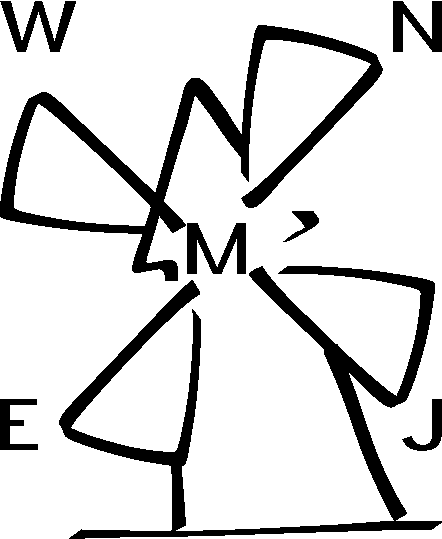
\includegraphics[width=1cm]{ nwejm-logo-NB }
}
\hbox_set_to_wd:Nnn \l_@@_journal_logo_box { 1cm }
{
  \box_move_down:nn
  {
    \box_ht:N \l_@@_journal_logo_box / 2
    -
    \box_ht:N \l_@@_journal_name_box / 2
  }
  {
    \box_use:N \l_@@_journal_logo_box
  }
}
\box_set_ht:Nn \l_@@_journal_logo_box { \c_zero_dim }
\box_set_dp:Nn \l_@@_journal_logo_box { \c_zero_dim }
}
%
\newpagestyle{@@_article_title_ps}[]{%
  % \widenhead{\c_zero_dim}{\c_zero_dim}
  \sethead%
  {
    \box_use:N \l_@@_journal_name_box
  }%
  {%
  }%
  {
    \box_use:N \l_@@_journal_logo_box
  }%
  %
  \setfoot%
  {}%
  {\thepage}%
  {}%
}
%    \end{macrocode}
%
% Patch needed in order entries of the framed TOC on back cover don't overlap
% the page numbers.
%    \begin{macrocode}
\def\@pnumwidth{\@tocrmarg}
%    \end{macrocode}
%
% \section{First pages}
%
% At begin of the document, we automatically :
% \begin{itemize}
% \item set the graphic path,
% \item set the page grid if the corresponding option has been passed,
% \item display of the front cover and the inside front cover.
% \end{itemize}
%
%    \begin{macrocode}
\AddToHook{begindocument}{%
  \graphicspath{{\c_@@_issue_images_path_string_tl//}{../\c_@@_issue_images_path_string_tl//}}
  % \glsdisablehyper
}
%    \end{macrocode}
%
% At the begin of document, we automatically switch to
% \begin{itemize}
% \item frontmatter\footnote{Mainly: page numbers in roman.} in the \enquote{issue}
%   version of the class (the first pages are for the table of contents which
%   was decided to be in frontmatter),
% \item mainmatter\footnote{Page numbers in arabic, right page style, right
%   geometry of the page.} in the \enquote{article} version of the class. In
%   this case, we also use the \enquote{main geometry} of the \enquote{issue}
%   version of the class, otherwise, the layouts of the two versions are likely
%   to be different.
% \end{itemize}
%    \begin{macrocode}
%<class-article>      \AddToHook{begindocument/end}{\g_@@_mainmatter_switch_tl}
%    \end{macrocode}
%
% \section{Options}
%
% In this section, options used by some of the document commands defined by the
% class are treated.
%
%    \begin{macrocode}
%</class|class-article>
%    \end{macrocode}
%
%    \begin{macrocode}
%<*class>
%    \end{macrocode}
%
% \subsection{Journal options}
%
% \begin{macro}{\l_@@_journal_publisher_tl}
% \begin{macro}{\l_@@_journal_address_tl}
% \begin{macro}{\l_@@_journal_phone_tl}
% \begin{macro}{\l_@@_journal_email_tl}
% \begin{macro}{\l_@@_journal_url_tl}
% \begin{macro}{\l_@@_journal_issn_tl}
% \begin{macro}{\l_@@_journal_isbn_tl}
% Some variables which are involved in options are created.
%    \begin{macrocode}
\tl_new:N \l_@@_journal_publisher_tl
\tl_new:N \l_@@_journal_address_tl
\tl_new:N \l_@@_journal_phone_tl
\tl_new:N \l_@@_journal_email_tl
\tl_new:N \l_@@_journal_url_tl
\tl_new:N \l_@@_journal_issn_tl
\tl_new:N \l_@@_journal_isbn_tl
%    \end{macrocode}
% \end{macro}
% \end{macro}
% \end{macro}
% \end{macro}
% \end{macro}
% \end{macro}
% \end{macro}
% \end{macro}
%
% \begin{macro}{publisher}
% \begin{macro}{address}
% \begin{macro}{phone}
% \begin{macro}{email}
% \begin{macro}{url}
% \begin{macro}{issn}
% \begin{macro}{isbn}
% The keys options are created.
%    \begin{macrocode}
\keys_define:nn { nwejm/journalsetup }
{
  publisher .tl_set:N = \l_@@_journal_publisher_tl,
  address .tl_set:N = \l_@@_journal_address_tl,
  phone .tl_set:N = \l_@@_journal_phone_tl,
  email .tl_set:N = \l_@@_journal_email_tl,
  url .tl_set:N = \l_@@_journal_url_tl,
  issn .tl_set:N = \l_@@_journal_issn_tl,
  isbn .tl_set:N = \l_@@_journal_isbn_tl,
%    \end{macrocode}
%
% All these options, when used, must receive a value.
%    \begin{macrocode}
  publisher .value_required:n = true,
  address .value_required:n = true,
  phone .value_required:n = true,
  email .value_required:n = true,
  url .value_required:n = true,
  issn .value_required:n = true,
  isbn .value_required:n = true,
}
%    \end{macrocode}
% \end{macro}
% \end{macro}
% \end{macro}
% \end{macro}
% \end{macro}
% \end{macro}
% \end{macro}
% \end{macro}
%
%    \begin{macrocode}
%</class>
%    \end{macrocode}
%
%    \begin{macrocode}
%<*class|class-article>
%    \end{macrocode}
%
% \subsection{Issues options}
%
% \begin{macro}{\g_@@_issue_number_int}
% \begin{macro}{\g_@@_issue_month_int}
% \begin{macro}{\g_@@_issue_year_int}
% Some variables which are involved in options are created.
%    \begin{macrocode}
\int_new:N \g_@@_issue_number_int
\int_new:N \g_@@_issue_month_int
\int_new:N \g_@@_issue_year_int
\tl_new:N \g_@@_frontcover_image_options_tl
%    \end{macrocode}
% \end{macro}
% \end{macro}
% \end{macro}
%
% \begin{macro}{number}
% \begin{macro}{volume}
% The keys options are created.
%    \begin{macrocode}
\keys_define:nn { nwejm/issuesetup }
{
  number .int_gset:N = \g_@@_issue_number_int,
  volume .int_gset:N = \g_@@_issue_volume_int,
%    \end{macrocode}
%
% All these options, when used, must receive a value.
%    \begin{macrocode}
  volume .value_required:n = true,
%    \end{macrocode}
%
% If "number" option is not used, its initial value is set to $0$.
% number.
%    \begin{macrocode}
  volume .initial:n = 0,
}
%    \end{macrocode}
%
% \end{macro}
% \end{macro}
%
% \subsection{Dates options}
%
% \begin{macro}{received}
% \begin{macro}{accepted}
% \begin{macro}{online}
% Some keys options for article's dates are created:
%    \begin{macrocode}
\keys_define:nn { nwejm/dates }
{
  received   .code:n = {
    \tl_gset:Nn \g_@@_reception_date_tl {#1}
    \bool_gset_true:N \g_@@_date_specified_bool
  },
  accepted   .code:n = {
    \tl_gset:Nn \g_@@_acception_date_tl {#1}
    \bool_gset_true:N \g_@@_date_specified_bool
  },
  online   .code:n = {
    \tl_gset:Nn \g_@@_online_date_tl {#1}
    \bool_gset_true:N \g_@@_date_specified_bool
  },
%    \end{macrocode}
%
% The following options, when used, must receive a value.
%    \begin{macrocode}
  received .value_required:n = true,
  accepted .value_required:n = true,
  online   .value_required:n = true,
}
%    \end{macrocode}
% \end{macro}
% \end{macro}
% \end{macro}
%
% \subsection{Authors options}
%
%    \begin{macrocode}
\quark_new:N \q_@@
\int_new:N \l_author_int
\prop_new:N \g_authors_prop
\prop_new:N \l_affiliations_tagged_prop
\cs_generate_variant:Nn \prop_put_if_new:Nnn { NVn }
\cs_generate_variant:Nn \prop_gput_if_new:Nnn { Nxn }
\cs_generate_variant:Nn \prop_put_if_new:Nnn { NnV }
%    \end{macrocode}
%
% Currently, \Package{expl3} doesn't provide any command that counts the number
% of items of property lists. It should be implemented soonish and, meanwhile,
% Bruno Le Floch provided the following macros (see
% \url{https://github.com/latex3/latex3/issues/293}).
%    \begin{macrocode}
\cs_new:Npn \__@@_prop_count:nn #1#2 { + 1 }
\cs_new:Npn \@@_prop_count:N #1
{ \int_eval:n { 0 \prop_map_function:NN #1 \__@@_prop_count:nn } }
%    \end{macrocode}
%
% \begin{macro}{affiliation}
% \begin{macro}{affiliationtagged}
% The keys options are created.
%    \begin{macrocode}
\NewDocumentCommand \@@_author_affiliation:ww { o u\q_@@ }
{
  \stepcounter{footnote}
  \prop_put_if_new:NVn \l_tmpa_prop {\the\c@footnote} {#2}
  \IfValueT{#1}{%
    \prop_put_if_new:NnV \l_affiliations_tagged_prop {#1} {\the\c@footnote}
  }
}
%
\keys_define:nn { nwejm / authors }
{
  email .tl_gset:N = \g_@@_people_email_tl,
  affiliation .code:n = {%
    \@@_author_affiliation:ww #1 \q_@@
  },
  affiliationtagged .code:n = {%
    \prop_get:NnNTF \l_affiliations_tagged_prop {#1} \l_tmpa_tl
    {%
      \prop_put_if_new:NVn \l_tmpa_prop {\l_tmpa_tl} {}
    }{
      \msg_error:nnn{@@}{Unknown~tag}{#1}
    }
  },
%    \end{macrocode}
%
% All these options, when used, must receive a value.
%    \begin{macrocode}
  affiliation .value_required:n = true,
  affiliationtagged .value_required:n = true,
}
%    \end{macrocode}
% \end{macro}
% \end{macro}
%
% \subsection{New theorem options}
%
%    \begin{macrocode}
\tl_new:N \l_@@_newtheorem_style_tl
\keys_define:nn { nwejm / newtheorem }
{
  title .tl_set:N = \l_@@_newtheorem_title_tl,
  title / french .tl_set:N = \l_@@_newtheorem_french_title_tl,
  title / english .tl_set:N = \l_@@_newtheorem_english_title_tl,
  title / german .tl_set:N = \l_@@_newtheorem_german_title_tl,
  title / dutch .tl_set:N = \l_@@_newtheorem_dutch_title_tl,
  title .value_required:n = true,
  title / french .value_required:n = true,
  title / english .value_required:n = true,
  title / german .value_required:n = true,
  title / dutch .value_required:n = true,
  %
  title-plural .tl_set:N = \l_@@_newtheorem_title_plural_tl,
  title-plural / french .tl_set:N = \l_@@_newtheorem_french_title_plural_tl,
  title-plural / english .tl_set:N = \l_@@_newtheorem_english_title_plural_tl,
  title-plural / german .tl_set:N = \l_@@_newtheorem_german_title_plural_tl,
  title-plural / dutch .tl_set:N = \l_@@_newtheorem_dutch_title_plural_tl,
  title-plural .value_required:n = true,
  title-plural / french .value_required:n = true,
  title-plural / english .value_required:n = true,
  title-plural / german .value_required:n = true,
  title-plural / dutch .value_required:n = true,
  %
  style .choice:,
  style / theorem .code:n = {\_@@_theorem_style:n {theorem}},
  style / definition .code:n = {\_@@_theorem_style:n {definition}},
  style / proof .code:n = {\_@@_theorem_style:n {proof}},
  style / unknown .code:n =
  \msg_error:nnxxx { nwejm } { Unknown~choice }
  { style } % Name of choice key
  { theorem~or~definition~or~proof } % Valid choices
  { \exp_not:n {#1} } % Invalid choice given
}
%    \end{macrocode}
% \end{macro}
% \end{macro}
% \end{macro}
%
%    \begin{macrocode}
\bool_new:N \g_@@_gradient_nabla_bool
\bool_new:N \g_@@_gradient_nabla_control_bool
\keys_define:nn { nwejm/articlesetup }
{
  gradient .choice:,
  gradient / nabla .code:n = {\bool_gset_true:N \g_@@_gradient_nabla_bool},
  gradient / grad .code:n = {\bool_gset_false:N \g_@@_gradient_nabla_bool},
  gradient / unknown .code:n =
  \msg_error:nnxxx { nwejmart } { Unknown~choice }
  { gradient } % Name of choice key
  { nabla~or~grad } % Valid choices
  { \exp_not:n {#1} } % Invalid choice given
}
%    \end{macrocode}
%
% \section{Miscellaneous token lists}
%
% We define some token lists for the long and short forms of the journal.
%    \begin{macrocode}
\tl_new:N \g_@@_nwejm_short_string_tl
\tl_new:N \g_@@_nwejm_string_tl
\tl_gset:Nn \g_@@_nwejm_short_string_tl {
  \cs_if_exist:cTF {texorpdfstring}
  {
    \texorpdfstring{\emph{\c_@@_journal_short_title_string_tl}}{\c_@@_journal_short_title_string_tl}
  }{%
    \emph{\c_@@_journal_short_title_string_tl}
  }%
}
\tl_gset:Nn \g_@@_nwejm_string_tl {
  \cs_if_exist:cTF {texorpdfstring}
  {
    \texorpdfstring{\emph{\c_@@_journal_title_string_tl}}{\c_@@_journal_title_string_tl}
  }{%
    \emph{\c_@@_journal_title_string_tl}
  }%
}
%    \end{macrocode}
%
%    \begin{macrocode}
\cs_new_protected:Nn \_@@_email:n
  {
    \href{mailto:#1}{\nolinkurl{#1}}%
  }
%    \end{macrocode}
%
% We create a control sequence that populates the bib file.
%    \begin{macrocode}
\tl_new:N \l_@@_crossref_tl
\cs_new_protected:Nn \_@@_populate_bib_file:nn
{
  \int_if_exist:cF {g_@@_#2_int}
  {
    \int_new:c {g_@@_#2_int}
  }
  \int_incr:c {g_@@_#2_int}
  \tl_if_in:nnTF { #2 } { author } {
    \tl_set:Nn \l_@@_crossref_tl {%
      \c_@@_issue_bib_key_tl
      -art-
      \int_use:N \g_@@_articles_int
    }
  } {
    \tl_set:Nn \l_@@_crossref_tl {\c_@@_issue_bib_key_tl}
  }
  \tl_set:Nn \l_@@_people_first_last_name_tl {#1}
  \iow_now:Nx \g_@@_bib_out_iow {%
    @article{
      \c_@@_issue_bib_key_tl -#2- \int_use:c {g_@@_#2_int},
      \iow_newline:
      author={\exp_not:V\l_@@_people_first_last_name_tl},
      \iow_newline:
      options={skipbib},
      \iow_newline:
      crossref  = {\l_@@_crossref_tl}
      \iow_newline:
    }
    \iow_newline:
  }%
}
%    \end{macrocode}
%
%    \begin{macrocode}
%</class|class-article>
%    \end{macrocode}
%
%    \begin{macrocode}
%<*class>
%    \end{macrocode}
%
% \section{Functions for specifiying the people involved in the journal}
%
% For this, and thanks to \Pkg{datatool}, we create a database of
% \enquote{people} involved in the journal.
%    \begin{macrocode}
\DTLnewdb{people}
%    \end{macrocode}
%
% Then we create the internal "\_@@_people" function that let us populate the
% "_@@_people" database. Each people will be identified by some identifiers:
% speciality (optional), firstname, lastname, affiliation, email, role.
%    \begin{macrocode}
\cs_new_protected:Nn \_@@_people:nnnnn
{
  \DTLnewrow{people}%
  \DTLnewdbentry{people}{first-last-name}{#1}%
  \DTLnewdbentry{people}{affiliation}{#2}%
  \DTLnewdbentry{people}{country}{#3}%
  \DTLnewdbentry{people}{email}{#4}%
  \DTLnewdbentry{people}{role}{#5}%
  \_@@_populate_bib_file:nn {#1}{#5}
}
%    \end{macrocode}
%
% We create a variant of this control sequence that passes the \emph{values} of
% the variables involved (see
% \url{http://tex.stackexchange.com/a/214284/18401}).
%    \begin{macrocode}
\cs_generate_variant:Nn \_@@_people:nnnnn { nVnVx }
%    \end{macrocode}
%
% \section{Functions for displaying people involved in the journal by role}
%
% We create the function that displays firstname and lastname of people involved
% in the journal by role.
%    \begin{macrocode}
\cs_new_protected:Nn \@@_display_people_by_role:n
{
  \DTLforeach*[\DTLiseq{\l_@@_people_role_tl}{#1}]{people}{%
    \l_@@_firstlastname_tl=first-last-name%
    ,\l_@@_people_affiliation_tl=affiliation%
    ,\l_@@_people_country_tl=country%
    ,\l_@@_people_email_tl=email%
    ,\l_@@_people_role_tl=role%
  }{%
    \tl_if_in:NnTF \l_@@_people_role_tl { editor } {
    \item[
      \_@@_citeauthor_no_giveninits:n {\c_@@_issue_bib_key_tl -#1- \exp_not:V\DTLcurrentindex}%
      ]
      \l_@@_people_affiliation_tl%
        \c_space_tl%
        (\l_@@_people_country_tl)%
      % ,\c_space_tl%
      % \_@@_email:n {\l_@@_people_email_tl}
      \DTLiflastrow{%
      }{%
        % \medskip%
      }
    }{
      \tl_if_in:NnTF \l_@@_people_role_tl { author } {
        \footnotesize%
        \noindent%
        \begin{description}[leftmargin=1em,style=nextline]
        \item[%
          \_@@_citeauthor_no_giveninits:n {\c_@@_issue_bib_key_tl -#1- \exp_not:V\DTLcurrentindex}%
          ]
          \tl_if_empty:NF \l_@@_people_affiliation_tl
          {%
            \mbox{}%
            \par%
            \vspace{-2ex}%
            \l_@@_people_affiliation_tl%
          }
          \tl_if_empty:NF \l_@@_people_email_tl
          {%
            \par%
            \_@@_email:n {\l_@@_people_email_tl}
          }
        \end{description}
        \DTLiflastrow{%
        }{
          \DTLpar%
          \medskip%
        }
      }{
        \tl_if_in:NnTF \l_@@_people_role_tl { publicationdirector } {
          \_@@_citeauthor_no_giveninits:n {\c_@@_issue_bib_key_tl -#1- \exp_not:V\DTLcurrentindex},~
          \l_@@_people_affiliation_tl%
        }{
          \_@@_citeauthor_no_giveninits:n {\c_@@_issue_bib_key_tl -#1- \exp_not:V\DTLcurrentindex}%
          \tl_if_empty:NF \l_@@_people_email_tl
          {
            \c_space_tl(\_@@_email:n {\l_@@_people_email_tl})
          }
        }
      }
    }
  }
}
%    \end{macrocode}
%
% \section{Displaying the front cover}
%
% We create a control sequence for the binding text.
%    \begin{macrocode}
\cs_new_protected:Nn \_@@_binding_text:n
{
  \Large
  \color{white}
  \bfseries
  \sffamily
  \node[outer~sep=0pt,inner~sep=0pt,rotate=90] at (current~page.#1)
  {
    \maxsizebox*{!}{\c_@@_potential_bindingoffset_dim}{\c_@@_journal_title_string_tl}
  } ;
  \node[outer~sep=0pt,inner~sep=0pt,rotate=90,anchor=east] at
  ($ (current~page.south~#1)!.2!(current~page.north~#1) $)
  {
    \maxsizebox*{!}{\c_@@_potential_bindingoffset_dim}{\c_@@_frontcover_left_string_tl}
  } ;
  \node[outer~sep=0pt,inner~sep=0pt,rotate=90,anchor=west] at ($
  (current~page.south~#1)!.8!(current~page.north~#1) $)
  {
    \maxsizebox*{!}{\c_@@_potential_bindingoffset_dim}{\c_@@_issue_year_tl}
  } ;
}
\cs_new_protected:Nn \_@@_grWheelComplete:nn
{
  \begingroup%
  \setkeys[GR]{cl}{#1}%
  \grStar[#1]{#2}%
  \pgfmathsetcounter{tkz@gr@a}{#2-1}%
  \edef\tkz@auxctp{\thetkz@gr@a}%
  \foreach \ia in {0,...,\tkz@auxctp}%
  {\foreach \ib in {\ia,...,\tkz@auxctp}%
    {\Edge(\cmdGR@cl@prefix\ia)(\cmdGR@cl@prefix\ib)}%
  }%
  \endgroup%
}
%    \end{macrocode}
%
% We create the variable that displays the front cover.
%    \begin{macrocode}
\tl_new:N \g_@@_display_frontcover_tl%
\tl_gset:Nn \g_@@_display_frontcover_tl {%
  \bool_gset_true:N \g_@@_frontcover_bool
  \pagestyle{@@_frontcover_ps}%
  \exp_after:wN\newgeometry\exp_after:wN{\c_@@_frontcover_geometry_tl}%
  \begin{tikzpicture}[remember~picture,overlay]
    \NoAutoSpacing
    \begin{pgfonlayer}{background}
      \file_if_exist:nTF {\c_@@_cover_background_image_tl}{
        \node[anchor=north~east,outer~sep=0pt,inner~sep=0pt] at (current~page.north~east) {
          \reflectbox{%
            \includegraphics[width=\paperheight,height=\c_@@_paperwidth_dim,angle=90]{
              \c_@@_cover_background_image_tl
            }%
          }
        };
      }{
        \fill[_@@_cover_background_color_tl] (current~page.north~east) rectangle
        (current~page.south~west);
      }
    \end{pgfonlayer}
    \_@@_binding_text:n {east}
  \end{tikzpicture}
  \begin{tikzpicture}[
    remember~picture,
    overlay,
    shift={(current~page~text~area.center)},
    scale=0.5,
    every~node/.style={scale=0.5}
    ]
    \SetGraphShadeColor{white}{blue}{white}%
    \tikzset{%
      VertexStyle/.style = {%
        shape        = circle,%
        fill         = white,%
        minimum~size = 3.5cm,%
        draw%
      }%
    }%
    \SetVertexNoLabel%
    \_@@_grWheelComplete:nn {RA=9}{6}
    \AssignVertexLabel{a}{%
      
\includegraphics[height=25mm]{nwejm-fields-institute-logo},%
      
\includegraphics[height=25mm]{nwejm-federation-recherche-math-npdc-logo},%
      
\includegraphics[height=10mm]{nwejm-kwg-logo},%
      
\includegraphics[height=20mm]{nwejm-smf-logo},%
      
\includegraphics[height=12mm]{nwejm-sml-logo},%
      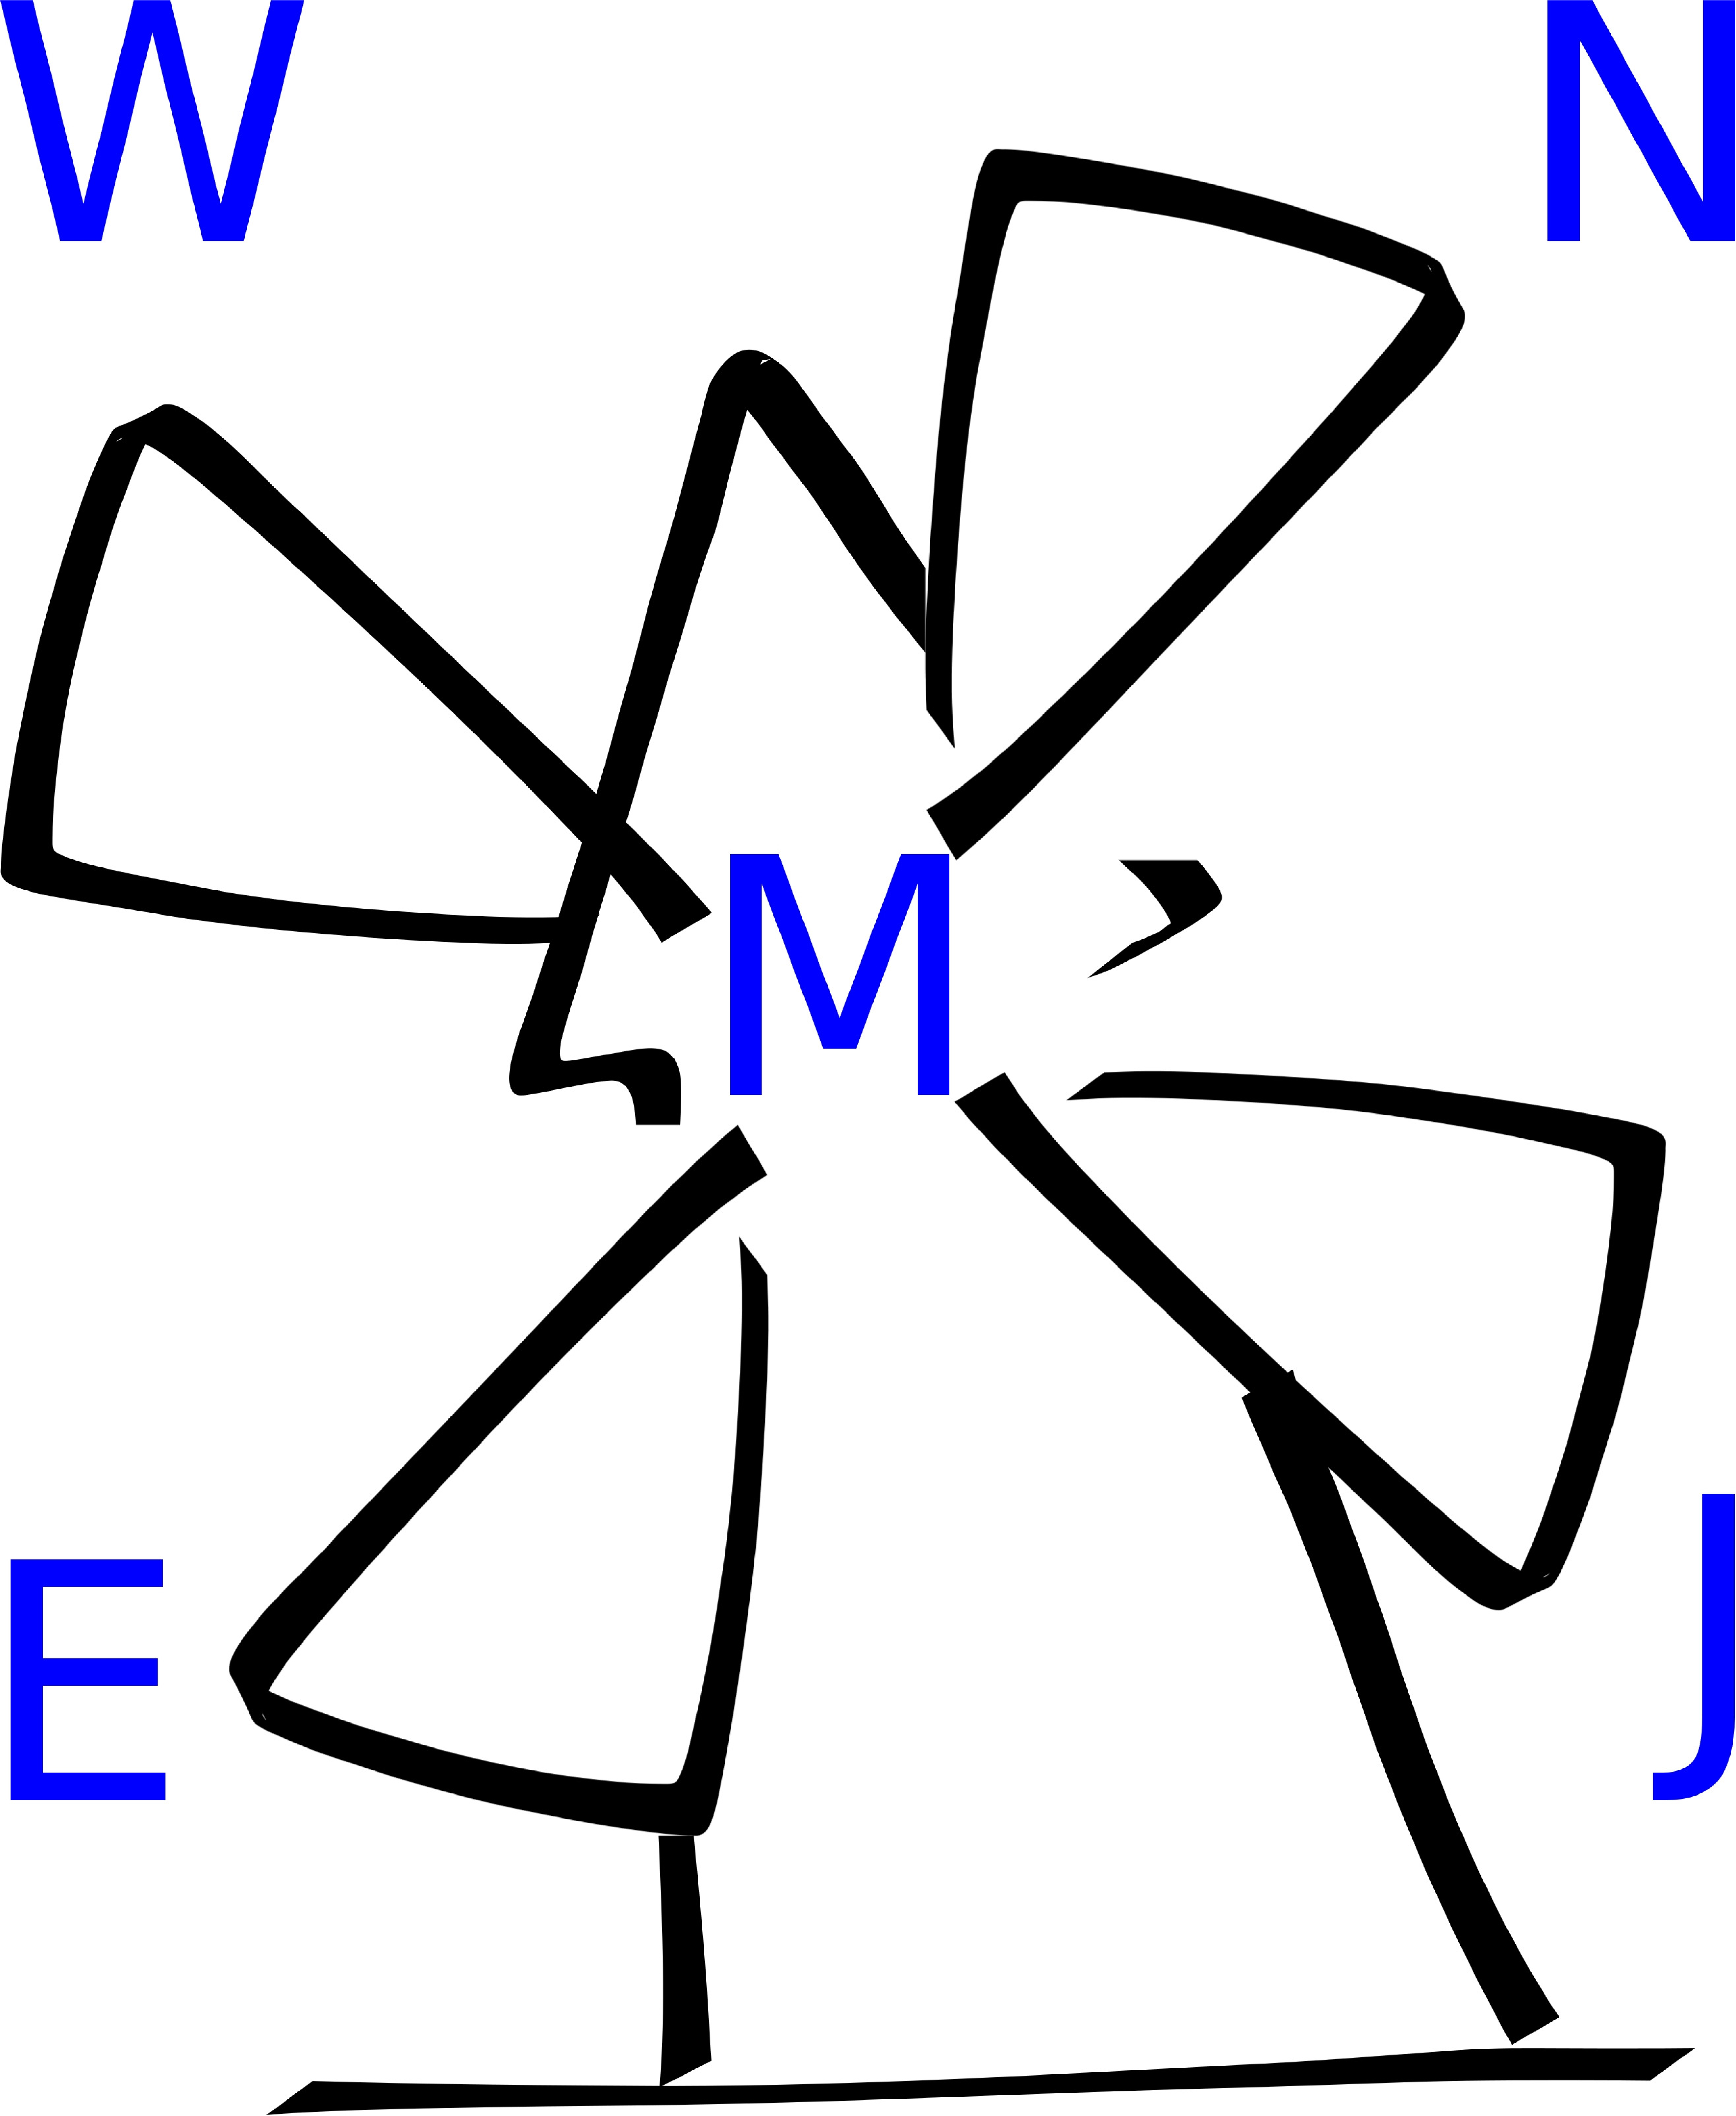
\includegraphics[height=25mm]{nwejm-logo}%
    };%
  \end{tikzpicture}
  \begin{tikzpicture}[remember~picture,overlay]
    % left horizontal lower white rule
    \fill[white]
    ([xshift=.95\c_@@_layoutwidth_dim,yshift=\c_@@_logos_rectangle_height_dim]current~page~text~area.south~west)
    rectangle
    ++(-.85\c_@@_layoutwidth_dim,\c_@@_logos_rectangle_thickness_dim)
    ;
    % left vertical white rule
    \fill[white]
    ([xshift=10mm,yshift=\c_@@_logos_rectangle_height_dim]current~page~text~area.south~west)
    rectangle
    ([xshift=10mm-\c_@@_logos_rectangle_thickness_dim,yshift=-\c_@@_logos_rectangle_height_dim+\c_@@_logos_rectangle_thickness_dim]current~page~text~area.north~west) ;
    % left horizontal upper white rule
    \fill[white]
    ([xshift=.95\c_@@_layoutwidth_dim,yshift=-\c_@@_logos_rectangle_height_dim+\c_@@_logos_rectangle_thickness_dim]current~page~text~area.north~west)
    rectangle
    ([xshift=.6\c_@@_layoutwidth_dim,yshift=-\c_@@_logos_rectangle_height_dim]current~page~text~area.north~west) ;
    % crop marks
    \draw [white]
    ([xshift=-2.5mm]current~page~text~area.north~west) --
    ([xshift=-7.5mm]current~page~text~area.north~west);
    \draw [white]
    ([yshift=2.5mm]current~page~text~area.north~west) --
    ([yshift=7.5mm]current~page~text~area.north~west);
    \draw [white]
    ([xshift=-2.5mm]current~page~text~area.south~west) --
    ([xshift=-7.5mm]current~page~text~area.south~west);
    \draw [white]
    ([yshift=-2.5mm]current~page~text~area.south~west) --
    ([yshift=-7.5mm]current~page~text~area.south~west);
    % binding limit
    \bool_if:NT {\g_@@_show_binding_bool} {
      \draw[green]
      ([xshift=-.5\c_@@_potential_bindingoffset_dim]current~page.north~east) --
      ([xshift=-.5\c_@@_potential_bindingoffset_dim]current~page.south~east);
    }
  \end{tikzpicture}
  \clearpage%
  \bool_gset_false:N \g_@@_frontcover_bool
}
%    \end{macrocode}
%
% \section{Displaying the inside front cover}
%
% We create the variable that displays the inside front cover.
%    \begin{macrocode}
\tl_new:N \g_@@_display_inside_frontcover_tl%
\tl_gset:Nn \g_@@_display_inside_frontcover_tl {%
  \bool_gset_true:N \g_@@_inside_frontcover_bool%
  \pagestyle{_@@_inside_cover_ps}%
  \exp_after:wN\newgeometry\exp_after:wN{%
    \c_@@_inside_cover_geometry_tl
    ,outer=\c_@@_outermargin_inside_frontcover_dim
  }%
  % \tikz[remember~picture,overlay] {%
  %   \draw [green]
  %   (current~page~text~area.south~west)
  %   rectangle
  %   (current~page~text~area.north~east)
  %   ;
  % }
  \setlist[description,1]{font=\scshape\bfseries}
  \footnotesize%
  \begin{multicols*}{2}
    \raggedright
      \setlength{\columnsep}{1mm}
      \begin{description}[leftmargin=2em]
      \item[\c_@@_editorinchief_string_tl] \
        \begin{description}[leftmargin=1em]
          \@@_display_people_by_role:n {editorinchief}
        \end{description}
        \bigskip
        \par
      \item[\c_@@_associate_editors_string_tl] \
        \begin{description}[leftmargin=1em]
          \@@_display_people_by_role:n {editor}
        \end{description}
        \bigskip
        \par
      \item[\c_@@_field_editor_string_tl] \
        \begin{description}[leftmargin=1em]
          \@@_display_people_by_role:n {fieldseditor}
        \end{description}
        \bigskip
        \par
      \item[\c_@@_managing_editor_string_tl] \
        \begin{description}[leftmargin=1em]
          \@@_display_people_by_role:n {managingeditor}
        \end{description}
      \end{description}
    \end{multicols*}
  \clearpage%
  \bool_gset_false:N \g_@@_inside_frontcover_bool
  \pagestyle{@@_frontmatter_ps}%
  \exp_after:wN\newgeometry\exp_after:wN{\c_@@_main_geometry_tl}%
}
%    \end{macrocode}
%
% \section{Displaying the inside back cover}
%
% We create the variable that displays the inside back cover.
%    \begin{macrocode}
\tl_new:N \g_@@_display_inside_backcover_tl%
\tl_gset:Nn \g_@@_display_inside_backcover_tl {%
  \bool_gset_true:N \g_@@_inside_backcover_bool%
  \pagestyle{_@@_inside_cover_ps}%
  \exp_after:wN\newgeometry\exp_after:wN{%
    \c_@@_inside_cover_geometry_tl
    ,outer=\c_@@_outermargin_inside_backcover_dim
  }%
  % \tikz[remember~picture,overlay] {%
  %   \draw [purple]
  %   (current~page~text~area.south~west)
  %   rectangle
  %   (current~page~text~area.north~east)
  %   ;
  % }
  \setlist[description,1]{font=\scshape\bfseries}
  \begin{description}[leftmargin=1em]
  \item[\c_@@_authors_instructions_string_tl{}:] \
    \g_@@_authors_instructions_tl
  \item[\c_@@_editorial_secretariat_string_tl{}:] \ \par%
    % \l_@@_journal_publisher_tl%
    % \par%
    % \c_space_tl\textendash{}\c_space_tl%
    \_@@_display_people_by_role:n { secretary }\par
    \l_@@_journal_address_tl\par%
    \c_@@_phone_string_tl{}:~\l_@@_journal_phone_tl{}\par%
    \_@@_email:n {\l_@@_journal_email_tl}
    \newline%
    % \c_space_tl\textendash{}\c_space_tl
    \url{\l_@@_journal_url_tl}
    \tl_if_empty:NF \l_@@_journal_issn_tl
    {%
    \item[\c_@@_issn_string_tl{}:] \l_@@_journal_issn_tl
    }
    \tl_if_empty:NF \l_@@_journal_isbn_tl
    {%
    \item[\c_@@_isbn_string_tl{}:] \l_@@_journal_isbn_tl
    }
  \item[\c_@@_latexclass_string_tl{}:]
    \_@@_display_people_by_role:n { classdesigner }
  \item[\c_@@_computer_engineering_string_tl{}:] %\g_@@_printer_text_tl
    \_@@_display_people_by_role:n { computerengineer }
  \item[\c_@@_graphicdesign_string_tl{}:] %\g_@@_graphicdesign_text_tl
    \_@@_display_people_by_role:n { graphicdesign }
  \end{description}
  \g_@@_font_designer_text_tl
  \par
  \vspace*{\stretch{1}}
  \selectlanguage{french}
  \shorthandon{;:!?}
  \begin{description}
  \item[\c_@@_publication_director_string_tl{}~:]
    \_@@_display_people_by_role:n { publicationdirector }
  \item[\c_@@_composed_by_string_tl{}~:]
    \_@@_display_people_by_role:n { composer }
  \end{description}
  \DTMlangsetup*{showdayofmonth=false}
  \centering
  \g_@@_masthead_tl
  \selectlanguage{english}
  \bool_gset_false:N \g_@@_inside_backcover_bool
}
%    \end{macrocode}
%
% \section{Displaying the back cover}
%
%    \begin{macrocode}
\tl_new:N \g_@@_short_toc_tl%
%    \end{macrocode}
%
%    \begin{macrocode}
\tl_new:N \g_@@_display_backcover_tl%
\tl_gset:Nn \g_@@_display_backcover_tl {%
  \bool_gset_true:N \g_@@_backcover_bool
  \exp_after:wN\newgeometry\exp_after:wN{%
    \c_@@_frontcover_geometry_tl
    ,layouthoffset=.5\c_@@_potential_bindingoffset_dim
  }%
  \bool_gset_true:N \g_@@_backcover_bool
  \begin{tikzpicture}[remember~picture,overlay]
    \NoAutoSpacing
    \begin{pgfonlayer}{background}
      \file_if_exist:nTF {\c_@@_cover_background_image_tl}{
        \node[anchor=north~west,outer~sep=0pt,inner~sep=0pt] at (current~page.north~west) {
          \includegraphics[width=\paperheight,height=\c_@@_paperwidth_dim,angle=90]{\c_@@_cover_background_image_tl}%
        };
      }{
        \fill[_@@_cover_background_color_tl] (current~page.north~east) rectangle
        (current~page.south~west);
      }
    \end{pgfonlayer}
    \_@@_binding_text:n {west}
  \end{tikzpicture}
  \noindent%
  \begin{tikzpicture}[remember~picture,overlay]
    % journal title
    \node [anchor=north,yshift=-\c_@@_layoutwidth_dim/20] at (current~page~text~area.north) {
      \begin{tcolorbox}[_@@_title_cover]
        North-Western~European\\[.5cm]
        Journal~of~Mathematics
      \end{tcolorbox}
    };
    % circular node for NWEJM logo
    \node[anchor=center,circle,fill=white,minimum~size=8.2cm] at
    ([yshift=-\c_@@_layoutheight_dim/2]current~page~text~area.north)
    {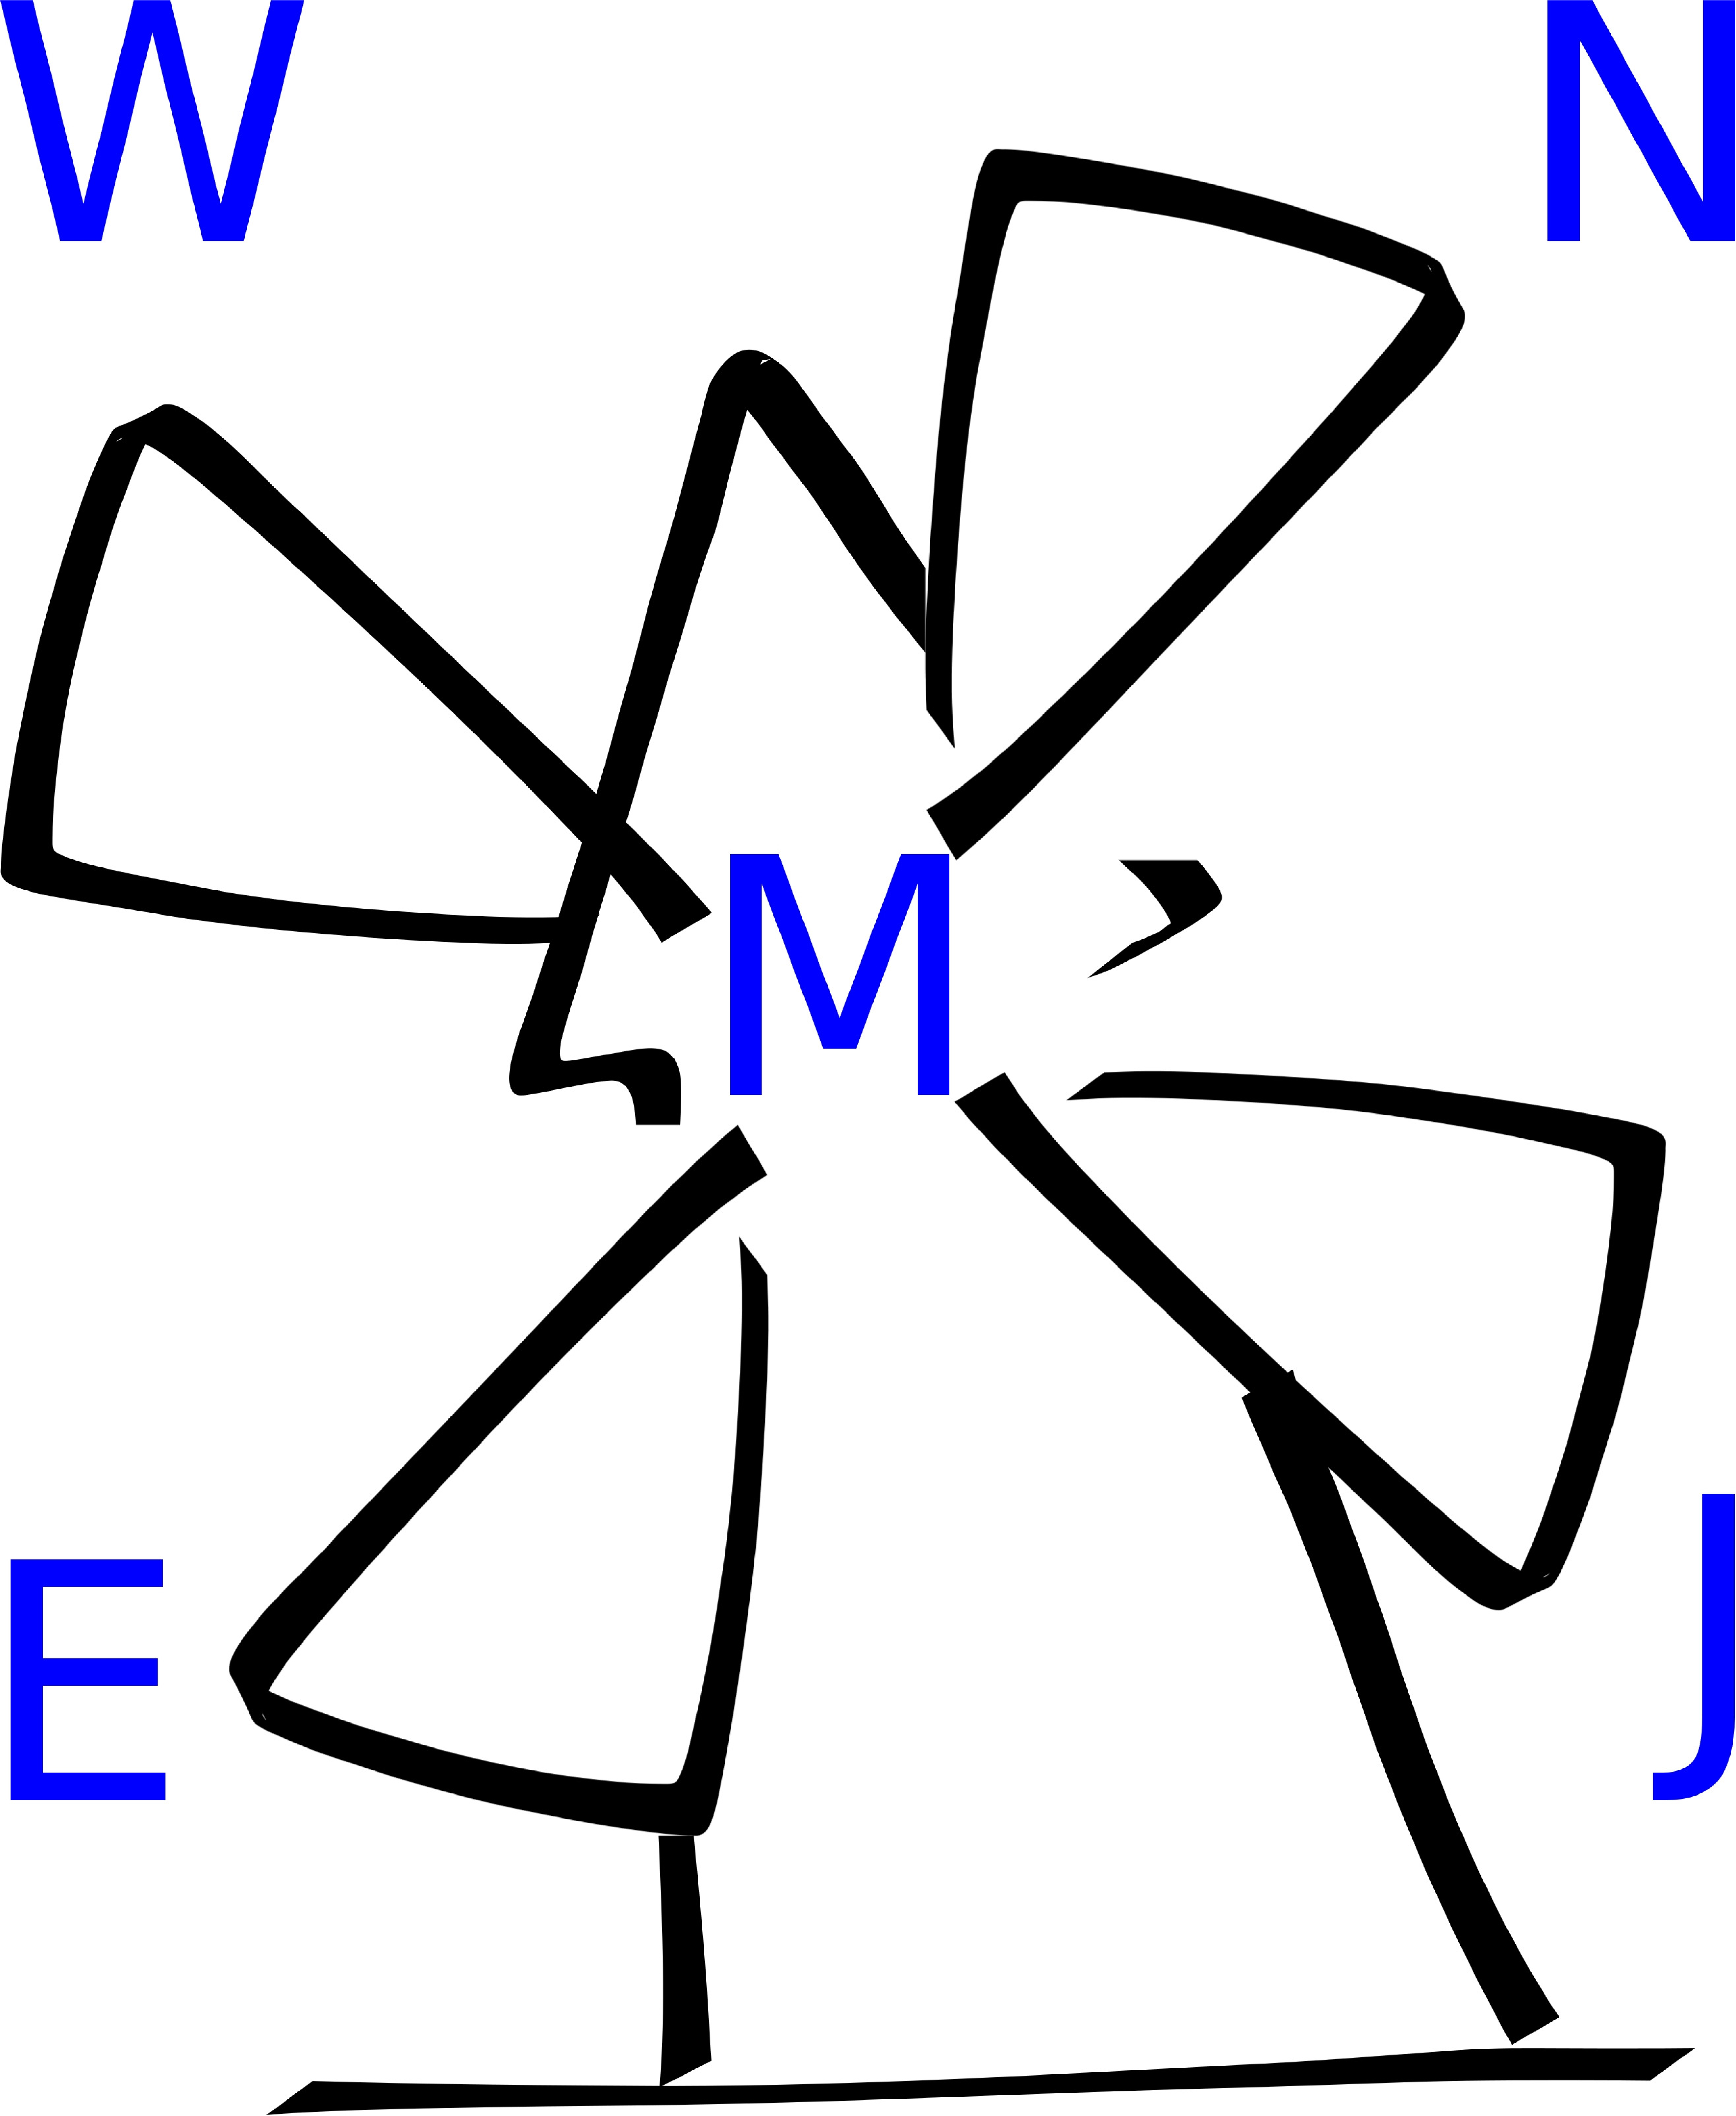
\includegraphics[height=5.5cm]{nwejm-logo}};
    % right vertical white rule
    \fill[white]
    ([xshift=-10mm,yshift=\c_@@_logos_rectangle_height_dim]current~page~text~area.south~east)
    rectangle
    ([xshift=-10mm+\c_@@_logos_rectangle_thickness_dim,yshift=\c_@@_logos_rectangle_height_dim+14cm]current~page~text~area.south~east) ;
    % right horizontal white rule
    \fill[white]
    ([yshift=\c_@@_logos_rectangle_height_dim+\c_@@_logos_rectangle_thickness_dim]current~page~text~area.south~west)
    rectangle
    ([xshift=.35\c_@@_layoutwidth_dim,yshift=\c_@@_logos_rectangle_height_dim]current~page~text~area.south~west) ;
    % number and year node
    \node[anchor=base~east] at
    ([xshift=-1.2cm,yshift=\c_@@_logos_rectangle_height_dim]current~page~text~area.south~east)
    {\color{white}\bfseries\sffamily\c_@@_frontcover_string_tl} ;
    % % white rectangle for university and laboratory logos
    \fill [white]
    ([yshift=\c_@@_logos_rectangle_height_dim-7.5mm]current~page~text~area.south~west)
    rectangle (current~page.south~east);
    % laboratory logo
    \node[anchor=south~east] at ([xshift=-10mm]current~page~text~area.south~east)
    {\includegraphics[height=.5\c_@@_logos_rectangle_height_dim]{logo-painleve}} ;
    % university logo
    \node[anchor=south~west] at (current~page~text~area.south~west)
    {
\includegraphics[height=.5\c_@@_logos_rectangle_height_dim]{ul-fst-math}} ;
    % crop marks
    \draw [white]
    ([xshift=2.5mm]current~page~text~area.north~east) --
    ([xshift=7.5mm]current~page~text~area.north~east);
    \draw [white]
    ([yshift=2.5mm]current~page~text~area.north~east) --
    ([yshift=7.5mm]current~page~text~area.north~east);
    \draw
    ([xshift=2.5mm]current~page~text~area.south~east) --
    ([xshift=7.5mm]current~page~text~area.south~east);
    \draw
    ([yshift=-2.5mm]current~page~text~area.south~east) --
    ([yshift=-7.5mm]current~page~text~area.south~east);
    % binding limit
    \bool_if:NT {\g_@@_show_binding_bool} {
      \draw[green]
      ([xshift=.5\c_@@_potential_bindingoffset_dim]current~page.north~west) --
      ([xshift=.5\c_@@_potential_bindingoffset_dim]current~page.south~west);
    }
  \end{tikzpicture}
}
%    \end{macrocode}
%
%    \begin{macrocode}
%</class>
%    \end{macrocode}
%
%    \begin{macrocode}
%<*class|class-article>
%    \end{macrocode}
%
% \section{Displaying the dates}
%
% We create the variable that displays the dates.
%    \begin{macrocode}
\cs_new_protected:Nn \_@@_date:nn
{
  \tl_if_exist:NT {#2}
  {
    \tl_if_empty:NF {#2}
    {
      \tl_if_eq:NNF {\c_@@_date_received_tl} {#1} { \c_@@_dates_separator_tl }
      \text_titlecase:n { \exp_args:No \GetTranslation{#1} }
      \c_@@_colon_tl\c_space_tl
      \DTMdate{#2}%
    }
  }
}
\tl_new:N \g_@@_display_dates_tl%
\tl_gset:Nn \g_@@_display_dates_tl {%
  \footnotesize%
  \_@@_date:nn {\c_@@_date_received_tl}{\g_@@_reception_date_tl}
  \_@@_date:nn {\c_@@_date_accepted_tl}{\g_@@_acception_date_tl}
  \_@@_date:nn {\c_@@_date_online_tl}  {\g_@@_online_date_tl}
  \tl_gclear:N \g_@@_reception_date_tl
  \tl_gclear:N \g_@@_acception_date_tl
  \tl_gclear:N \g_@@_online_date_tl
}
%    \end{macrocode}
%
% \section{Displaying the keywords}
%
% \begin{macro}{\keywords}
% \begin{macro}{\g_@@_keywords_tl}
%   The command for article's keywords is defined: the article's keywords is
%   store in "\g_@@_keywords_tl" for later use.
%    \begin{macrocode}
\tl_new:N \g_@@_keywords_tl
\NewDocumentCommand \keywords { O{} m } {
  \tl_gclear:N \g_@@_keywords_tl
  \tl_clear:N \l_tmpb_clist
  \clist_set:Nn \l_tmpb_clist {#2}
  \tl_set:Nx \g_@@_keywords_tl { \clist_use:Nnnn \l_tmpb_clist { ,~ } { ,~ } { ,~ } }
%<class-article>  \tl_if_empty:nTF {#1} {%
%<class-article>    \hypersetup{pdfkeywords={\g_@@_keywords_tl}}
%<class-article>  }{
%<class-article>    \clist_set:Nn \l_tmpb_clist {#1}
%<class-article>    \hypersetup{pdfkeywords={\clist_use:Nnnn \l_tmpb_clist { ,~ } { ,~ } { ,~ }}}
%<class-article>  }
}
%    \end{macrocode}
% \end{macro}
% \end{macro}
%
% \section{Displaying the Mathematical Subject Classification (\textsc{msc})}
%
% \begin{macro}{\msc}
% \begin{macro}{\g_@@_msc_tl}
%   The command for article's \textsc{msc} is defined: the article's \textsc{msc} is
%   store in "\g_@@_msc_tl" for later use.
%    \begin{macrocode}
\tl_new:N \g_@@_msc_tl
\NewDocumentCommand \msc { m } {
  \tl_gclear:N \g_@@_msc_tl
  \tl_clear:N \l_tmpa_clist
  \clist_set:Nn \l_tmpa_clist {#1}
  \tl_set:Nn \g_@@_msc_tl { \clist_use:Nnnn \l_tmpa_clist { ,~ } { ,~ } { ,~ } }
%%<class-article>    \hypersetup{pdfmsc=\g_@@_msc_tl}
}
%    \end{macrocode}
% \end{macro}
% \end{macro}
%
% \section{Page numbers' synchronization of standalone articles/issue}
%
% The machinery for page numbers' synchronization of standalone articles/issue
% needs the main file name to be fixed (chosen name: \enquote{issue}). If that's
% not the case an error is thrown.
%    \begin{macrocode}
%<class>\str_if_eq:eeTF  \c_sys_jobname_str \c_@@_main_file_name_tl {
%<class>  \bool_if:NT {\g_@@_cover_bool} {
%<class>    \msg_error:nn{nwejm}{Wrong~cover's~main~file~name!}
%<class>  }
%<class>}{
%<class>  \bool_if:NTF {\g_@@_cover_bool} {
%<class>    \file_if_exist:nTF { \c_@@_issue_number_year_file_string_tl }
%<class>    {
%<class>      \file_input:n {\c_@@_issue_number_year_file_string_tl}
%<class>    }{
%<class>      \msg_error:nn{nwejm}{Main~file~needs~to~be~compiled!}
%<class>    }
%<class>  }{
%<class>    \msg_error:nn{nwejm}{Wrong~issue's~main~file~name!}
%<class>  }
%<class>}
%    \end{macrocode}
%
%    \begin{macrocode}
%<class-article>
%<class-article>\file_if_exist:nT { \c_@@_main_file_name_tl.aux }
%<class-article>{\externaldocument[@@-]{\c_@@_main_file_name_tl}
%<class-article>  \AddToHook{begindocument/end}{\setcounter{page}{\number\numexpr\getpagerefnumber{@@-\currfilebase}}}
%<class-article>}
%    \end{macrocode}
%
% In case one wants to manually control the page numbers, the following macro
% ×\fixpagenumber{...}× has to be used instead of ×\setcounter{page}{...}×.
%    \begin{macrocode}
\NewDocumentCommand \fixpagenumber { m } {
%<class-article>\setcounter{page}{#1}
}
%    \end{macrocode}
%
% \section{User level commands}
%
% Here, we gather all the user level (public) commands.
%
%    \begin{macrocode}
%</class|class-article>
%    \end{macrocode}
%
%    \begin{macrocode}
%<*class>
%    \end{macrocode}
%
% \subsection{Populating the people involved in the journal}
%
% \begin{macro}{\editorinchief}
% \begin{macro}{\managingeditor}
% \begin{macro}{\fieldseditor}
% \begin{macro}{\editor}
% \begin{macro}{\classdesigner}
% \begin{macro}{\fontdesigner}
% \begin{macro}{\classmaintainer}
% \begin{macro}{\graphicdesign}
% \begin{macro}{\computerengineer}
% \begin{macro}{\secretary}
%   We define some document-level commands that let the user specify
%   respectively the editor(s) in chief, the fields editor, the managing editor,
%   the editors, the class designer and maintainer(s), etc.
%    \begin{macrocode}
\NewDocumentCommand \editorinchief {mmmm}
{
  \_@@_people:nnnnn {#1}{#2}{#3}{#4}{editorinchief}
}
\NewDocumentCommand \editor {mmmm}
{
  \_@@_people:nnnnn {#1}{#2}{#3}{#4}{editor}
}
\NewDocumentCommand \fieldseditor {mmmm}
{
  \_@@_people:nnnnn {#1}{#2}{#3}{#4}{fieldseditor}
}
\NewDocumentCommand \managingeditor {mmmm}
{
  \_@@_people:nnnnn {#1}{#2}{#3}{#4}{managingeditor}
}
\NewDocumentCommand \classdesigner {mmmm}
{
  \_@@_people:nnnnn {#1}{#2}{#3}{#4}{classdesigner}
}
\NewDocumentCommand \computerengineer {mmmm}
{
  \_@@_people:nnnnn {#1}{#2}{#3}{#4}{computerengineer}
}
\NewDocumentCommand \classmaintainer {mmmm}
{
  \_@@_people:nnnnn {#1}{#2}{#3}{#4}{classmaintainer}
}
\NewDocumentCommand \fontdesigner {mmmm}
{
  \_@@_people:nnnnn {#1}{#2}{#3}{#4}{fontdesigner}
}
\NewDocumentCommand \graphicdesign {mmmm}
{
  \_@@_people:nnnnn {#1}{#2}{#3}{#4}{graphicdesign}
}
\NewDocumentCommand \computerassistance {mmmm}
{
  \_@@_people:nnnnn {#1}{#2}{#3}{#4}{computerassistance}
}
\NewDocumentCommand \secretary {mmmm}
{
  \_@@_people:nnnnn {#1}{#2}{#3}{#4}{secretary}
}
\NewDocumentCommand \publicationdirector {mmmm}
{
  \_@@_people:nnnnn {#1}{#2}{#3}{#4}{publicationdirector}
}
\NewDocumentCommand \composer {mmmm}
{
  \_@@_people:nnnnn {#1}{#2}{#3}{#4}{composer}
}
%    \end{macrocode}
% \end{macro}
% \end{macro}
% \end{macro}
% \end{macro}
% \end{macro}
% \end{macro}
% \end{macro}
% \end{macro}
% \end{macro}
% \end{macro}
%
% \subsection{Issue setup}
%
% \begin{macro}{\issuesetup}
%   We define the command that lets the user specify the issue setup.
%    \begin{macrocode}
\NewDocumentCommand \issuesetup { m } {
%    \end{macrocode}
%
% Its keys are set (only "number", "month" and "year" are relevant here).
%    \begin{macrocode}
  \keys_set:nn { nwejm/issuesetup } {#1}
%    \end{macrocode}
%
% We use here the fact that, if the "number", "month" or "year" options are not
% used, their corresponding "\g_@@_issue_number_int", "\g_@@_issue_month_int" or
% "\g_@@_issue_year_int" variables are equal to $0$ ($<1$).
%
% First, if "number" is not used, its "\g_@@_issue_number_int" variable is set
% to "\c_@@_first_issue_number_int"\footnote{The number of the first journal's
% issue using the present class.} and a warning is emitted.
%    \begin{macrocode}
  \int_compare:nNnT {\g_@@_issue_number_int}<{1}
  {
    \int_gset:Nn \g_@@_issue_number_int { \c_@@_first_issue_number_int }
    \msg_warning:nnn{nwejm}{Issue~number~needed}{number}
  }
%    \end{macrocode}
%
% If not specified as \refCom{issuesetup}'s key-value options, issue's month and
% year are computed from issue number (which defaults to
% "\c_@@_first_issue_month_int").
%
% \begin{macro}{\c_@@_issue_age_in_months_int}
%   First, if "month" or "year" option is not used (one of the previous
%   variables is $0$ hence their product is $0$ ($<1$)), we compute the issue
%   age in months, useful for both month and year computation.
%    \begin{macrocode}
  \int_compare:nNnT {\g_@@_issue_month_int * \g_@@_issue_year_int}<{1}
  {
    \int_new:N \g_@@_issue_age_in_months_int%
    \int_gset:Nn \g_@@_issue_age_in_months_int
    {
      \c_@@_first_issue_month_int
      + \c_@@_interval_in_months_int
      * ( \int_use:N \g_@@_issue_number_int - \c_@@_first_issue_number_int )
    }
  }
%    \end{macrocode}
% \end{macro}
%
% If the "month" is not used, we replace "\g_@@_issue_month_int" ($=0$) by its
% computed value from the issue number.
%    \begin{macrocode}
  \int_compare:nNnT {\g_@@_issue_month_int}<{1}
  {
    \int_gset:Nn \g_@@_issue_month_int
    {
      \int_mod:nn { \g_@@_issue_age_in_months_int } { 12 }
    }
  }
%    \end{macrocode}
%
% If the "year" is not used, we replace "\g_@@_issue_year_int" ($=0$) by its
% computed value from the issue number.
%    \begin{macrocode}
  \int_compare:nNnT {\g_@@_issue_year_int}<{1}
  {
    \int_new:N \g_@@_issue_age_in_years_int%
    \int_gset:Nn \g_@@_issue_age_in_years_int
    {%
      \int_div_truncate:nn { \g_@@_issue_age_in_months_int } { 12 }
    }%
    \int_gset:Nn \g_@@_issue_year_int
    {
      \g_@@_issue_age_in_years_int + \c_@@_first_issue_year_int
    }
  }%
%    \end{macrocode}
%
% We fix some of the PDF's metadata.
%    \begin{macrocode}
  \bool_if:NT {\g_@@_cover_bool} {
    \hypersetup{
      pdftitle=\c_@@_journal_title_string_tl\c_space_tl--\c_space_tl\c_@@_frontcover_left_string_tl\c_space_tl--\c_space_tl\int_use:N\g_@@_issue_year_int,
      pdfauthor=\c_@@_journal_title_string_tl\c_space_tl(editor)
    }
  }
%    \end{macrocode}
%
% We write some data to an auxiliary file which be read by the file dedicated to
% the cover pages production.
%    \begin{macrocode}
  \iow_new:N   \g_@@_issue_number_year_out_iow
  \iow_open:Nn \g_@@_issue_number_year_out_iow {\c_@@_issue_number_year_file_string_tl}
  \iow_now:Nx \g_@@_issue_number_year_out_iow {
    \tl_const:Nn \token_to_str:N \c_@@_issue_number_tl {
      \int_eval:n {\g_@@_issue_number_int}
    }
    \iow_newline:
    \tl_const:Nn \token_to_str:N \c_@@_issue_year_tl {
      \int_eval:n {\g_@@_issue_year_int}
    }
  }
  \iow_close:N \g_@@_issue_number_year_out_iow
}
%    \end{macrocode}
% \end{macro}
%
% \subsection{Journal setup}
%
% \begin{macro}{\journalsetup}
%   We define the command that lets us specify the journal setup. This setup is
%   likely to be rarely changed.
%    \begin{macrocode}
\NewDocumentCommand \journalsetup { m } {
%    \end{macrocode}
%
% Its keys are set (only "publisher", "address", "phone", "email", "url"
% and "issn" are relevant here).
%    \begin{macrocode}
  \keys_set:nn { nwejm/journalsetup } { #1 }
}
%    \end{macrocode}
%
% \begin{macro}{\authorsinstructions}
%   We define the command that lets us specify the instructions to authors. This
%   setup is likely to be rarely changed.
%    \begin{macrocode}
\tl_new:N \g_@@_authors_instructions_tl
\NewDocumentCommand \authorsinstructions { +m } {
  \IfNoValueF {#1}
  {
    \tl_gset:Nn \g_@@_authors_instructions_tl {#1}
  }
}
%    \end{macrocode}
%
% \begin{macro}{\masthead}
%   We define the command that lets us specify the masthead (\enquote{ours} in French). This
%   setup is likely to be rarely changed.
%    \begin{macrocode}
\tl_new:N \g_@@_masthead_tl
\NewDocumentCommand \masthead { +m } {
  \IfNoValueF {#1}
  {
    \tl_gset:Nn \g_@@_masthead_tl {#1}
  }
}
%    \end{macrocode}
%
%    \begin{macrocode}
%</class>
%    \end{macrocode}
%
%    \begin{macrocode}
%<*class|class-article>
%    \end{macrocode}
%
% \end{macro}
%
% \subsection{\Pkg{Varioref}}
%
% We have to save the extra definitions of the \Pkg{varioref} which currently is
% multilingual aware.
%    \begin{macrocode}
\vref@addto\extrasfrench{%
  \def\reftextfaceafter {page~\reftextvario{ci-contre}{suivante}}%
  \def\reftextfacebefore{page~\reftextvario{ci-contre}%
    {pr\'ec\'edente}}%
  \def\reftextafter
  {page~suivante}%
  \def\reftextbefore
  {page~pr\'ec\'edente}%
  \def\reftextcurrent {de~la~pr\'esente~page}%
  \def\reftextfaraway#1{p.\nobreakspace\pageref{#1}}%
  \def\reftextpagerange#1#2{p.\nobreakspace\pageref{#1}--\pageref{#2}}%
  \def\reftextlabelrange#1#2{\ref{#1}~\‘a\nobreakspace\ref{#2}}%
}
\vref@addto\extrasngerman{%
  \def\reftextfaceafter {auf~der~n\"achsten~Seite}%
  \def\reftextfacebefore{auf~der~vorherigen~Seite}%
  \let\reftextafter     \reftextfaceafter
  \let\reftextbefore    \reftextfacebefore
  \def\reftextcurrent   {auf~dieser~Seite}%
  \def\reftextfaraway#1{auf~S.\nobreakspace\pageref{#1}}%
  \def\reftextpagerange#1#2{auf~den~S.\nobreakspace\pageref{#1}--\pageref{#2}}%
  \def\reftextlabelrange#1#2{\ref{#1}~bis\nobreakspace\ref{#2}}%
}
\vref@addto\extrasdutch{%
  \def\refpagename{pagina}%
  \def\reftextfaceafter {op~de~\reftextvario{rechter~\refpagename}%
    {\refpagename\ hiernaast}}%
  \def\reftextfacebefore{op~de~\reftextvario{linker~\refpagename}%
    {\refpagename\ hiernaast}}%
  \def\reftextafter     {op~de~\reftextvario{volgende~\refpagename}%
    {\refpagename\ hierna}}%
  \def\reftextbefore    {op~de~\reftextvario{vorige~\refpagename}%
    {\refpagename\ hiervoor}}%
  \def\reftextcurrent   {op~deze~\refpagename}%
  \def\reftextfaraway#1{op~\refpagename\nobreakspace\pageref{#1}}
}
\vref@addto\extrasenglish{%
  \def\reftextfaceafter {on~the~\reftextvario{facing}{next}~page}%
  \def\reftextfacebefore{on~the~\reftextvario{facing}{preceding}~page}%
  \def\reftextafter     {on~the~\reftextvario{following}{next}~page}%
  \def\reftextbefore    {on~the~\reftextvario{preceding}{previous}~page}%
  \def\reftextcurrent   {on~\reftextvario{this}{the~current}~page}%
  \def\reftextfaraway#1{on~p.\nobreakspace\pageref{#1}}%
  \def\reftextpagerange#1#2{on~pp.\nobreakspace\pageref{#1}--\pageref{#2}}%
  \def\reftextlabelrange#1#2{\ref{#1}~to\nobreakspace\ref{#2}}%
}
%    \end{macrocode}
%
% We don't want randomization in the \package{varioref} expressions in order to
% reduce discrepancies between the whole issue and the individual articles.
%    \begin{macrocode}
\def\reftextvario#1#2{#2}
%    \end{macrocode}
%
% \subsection{Article setup}
%
% Some of the document commands will be restricted to document body, as the
% following ×\articlesetup× command whose effects would otherwise be overriden
% when, for the whole issue, preambles of each article will be gathered thanks
% to \Pkg{standalone}.
%    \begin{macrocode}
\cs_new_protected:Nn \_@@_command_only_in_body:n
{
  \cs_if_eq:NNF {\@onlypreamble} {\@notprerr} {
    \msg_error:nnn{
%<class-article>     nwejmart
%<class>     nwejm
     }{Command~restricted~to~document~body~used~in~preamble}{#1}
  }
}
%    \end{macrocode}
%
% \begin{macro}{\articlesetup}
%   We define the command that lets the user specify the article setup.
%    \begin{macrocode}
\NewDocumentCommand \articlesetup { m } {
  \_@@_command_only_in_body:n {\articlesetup}
  \keys_set:nn { nwejm/articlesetup } {#1}
}
%    \end{macrocode}
% \end{macro}
%
% \subsection{Dates setup}
%
% \begin{macro}{\dates}
%   We define the command that lets the user specify the issue setup.
%    \begin{macrocode}
\NewDocumentCommand \dates { m } {
  \keys_set:nn { nwejm/dates } { #1 }
}
%    \end{macrocode}
% \end{macro}
%
% Because of the ×capitalize× option passed to \Package{cleveref}, the names of
% the references (\enquote{chapter}, \enquote{theorem}, etc.) have their first
% letter capitalised (even with ×\cref×), which fit the English/Amercian
% typographic rules, but not the French ones. Hence, we redefine these
% references' names in French in order ×\cref× gives their lower case
% version. Because this redefinition is needed more than once, we store it in
% the ×\g_@@_french_crefname_tl× token list.
%    \begin{macrocode}
\tl_gset:Nn \g_@@_french_crefname_tl {
  \clist_set:Nn \l_tmpa_clist {%
    theorem,
    corollary,
    conjecture,
    proposition,
    lemma,
    axiom,
    definition,
    remark,
    example,
    notation,
    proof%
  }
  \clist_map_inline:Nn \l_tmpa_clist {
    \crefname{#1}{
      \text_lowercase:n{
        \GetTranslationFor{french}{#1}
      }
    }{%
      \text_lowercase:n{
        \GetTranslationFor{french}{plural-#1}
      }
    }
  }
  \crefname{equation}{{\'e}quation}{{\'e}quations}%
  \crefname{figure}{figure}{figures}%
  \crefname{table}{table}{tables}%
  \crefname{page}{page}{pages}%
  \crefname{part}{partie}{parties}%
  \crefname{chapter}{chapitre}{chapitres}%
  \crefname{section}{section}{sections}%
  \crefname{appendix}{annexe}{annexes}%
  \crefname{enumi}{point}{points}%
  \crefname{footnote}{note}{notes}%
  \crefname{theorem}{th\'eor\`eme}{th\'eor\`emes}%
  \crefname{lemma}{lemme}{lemmes}%
  \crefname{corollary}{corollaire}{corollaires}%
  \crefname{proposition}{proposition}{propositions}%
  \crefname{definition}{d\'efinition}{d\'efinitions}%
  \crefname{result}{r\'esultat}{r\'esultats}%
  \crefname{example}{exemple}{exemples}%
  \crefname{remark}{remarque}{remarques}%
  \crefname{note}{commentaire}{commentaires}%
  \crefname{algorithm}{algorithme}{algorithmes}%
  \crefname{listing}{liste}{listes}%
  \crefname{line}{ligne}{lignes}%
}
%    \end{macrocode}
%
%    \begin{macrocode}
%</class|class-article>
%    \end{macrocode}
%
%    \begin{macrocode}
%<*class>
%    \end{macrocode}
%
% \subsection{Input variant}
%
% We create a variant of the "\input" macro to be use for the input of each
% article: it starts a new \package{biblatex}'s "refsection" and reset to zero
% some counters. It also redefine the glossaries' rules since glossaries'
% acronyms' suffix in effect are not for the last loaded language (see
% \url{https://tex.stackexchange.com/q/475788/18401}).
%    \begin{macrocode}
\NewDocumentCommand \inputarticle { O{english} m } {%
%    \end{macrocode}
%
% First, we don't want the (next) title to appear in the headers of the preceding
% article.
%    \begin{macrocode}
  \cleardoublepage
  \int_gincr:N \g_@@_articles_int
  \newrefsection
  \renewcommand*{\glspluralsuffix}{s}
  \renewcommand*{\glsacrpluralsuffix}{\glspluralsuffix}
  \renewcommand*{\glsupacrpluralsuffix}{\glstextup{\glsacrpluralsuffix}}
  \StandardFootnotes
  \str_case:nn {#1} {
    {english} {
      \selectlanguage{english}
      % \shorthandoff{"}%
      \renewcommand*{\glossaryname}{Glossary}%
      \renewcommand*{\acronymname}{Acronyms}%
      \renewcommand*{\entryname}{Notation}%
      \renewcommand*{\descriptionname}{Description}%
      \renewcommand*{\symbolname}{Symbol}%
      \renewcommand*{\pagelistname}{Page List}%
      \renewcommand*{\glssymbolsgroupname}{Symbols}%
      \renewcommand*{\glsnumbersgroupname}{Numbers}%
    }
    {german} {
      \selectlanguage{ngerman}
      % \shorthandon{"}%
      \renewcommand*{\glossaryname}{Glossar}%
      \renewcommand*{\acronymname}{Akronyme}%
      \renewcommand*{\entryname}{Bezeichnung}%
      \renewcommand*{\descriptionname}{Beschreibung}%
      \renewcommand*{\symbolname}{Symbol}%
      \renewcommand*{\pagelistname}{Seiten}%
      \renewcommand*{\glssymbolsgroupname}{Symbole}%
      \renewcommand*{\glsnumbersgroupname}{Zahlen}%
    }
    {ngerman} {
      \selectlanguage{ngerman}
      % \shorthandon{"}%
      \renewcommand*{\glossaryname}{Glossar}%
      \renewcommand*{\acronymname}{Akronyme}%
      \renewcommand*{\entryname}{Bezeichnung}%
      \renewcommand*{\descriptionname}{Beschreibung}%
      \renewcommand*{\symbolname}{Symbol}%
      \renewcommand*{\pagelistname}{Seiten}%
      \renewcommand*{\glssymbolsgroupname}{Symbole}%
      \renewcommand*{\glsnumbersgroupname}{Zahlen}%
    }
    {french} {
      \selectlanguage{french}
      % \shorthandoff{"}%
%    \end{macrocode}
%
% Though we switch to \pkg{babel}'s ×french×, footnotes are not displayed as
% French ones in the issue. The following fixes this trouble.
%    \begin{macrocode}
      \FrenchFootnotes
      \g__nwejm_french_crefname_tl
      \renewcommand*{\glossaryname}{Glossaire}%
      \renewcommand*{\acronymname}{Acronymes}%
      \renewcommand*{\entryname}{Terme}%
      \renewcommand*{\descriptionname}{Description}%
      \renewcommand*{\symbolname}{Symbole}%
      \renewcommand*{\pagelistname}{Pages}%
      \renewcommand*{\glssymbolsgroupname}{Symboles}%
      \renewcommand*{\glsnumbersgroupname}{Nombres}%
      \renewcommand*{\glspluralsuffix}{s}
      \renewcommand*{\glsacrpluralsuffix}{}
      \renewcommand*{\glsupacrpluralsuffix}{}
    }
    {dutch} {
      \selectlanguage{dutch}
      % \shorthandon{"}%
      \renewcommand*{\glossaryname}{Woordenlijst}%
      \renewcommand*{\acronymname}{Acroniemen}%
      \renewcommand*{\entryname}{Benaming}%
      \renewcommand*{\descriptionname}{Beschrijving}%
      \renewcommand*{\symbolname}{Symbool}%
      \renewcommand*{\pagelistname}{Pagina's}%
      \renewcommand*{\glssymbolsgroupname}{Symbolen}%
      \renewcommand*{\glsnumbersgroupname}{Cijfers}%
    }
  }%
%    \end{macrocode}
%
% We reset setup possibly chosen in previous articles.
%    \begin{macrocode}
%<class>  \bool_gset_false:N \g_@@_gradient_nabla_bool
%<class>  \bool_gset_false:N \g_@@_gradient_nabla_control_bool
%<class>  \bool_gset_false:N \g_@@_grad_used_bool
%    \end{macrocode}
%
%    \begin{macrocode}
  \inputfrom{./}{#2}
%    \end{macrocode}
% The list of counters we want to be able to easily set to zero doesn't contains
% only the ones associated to the (numbered) theorem environments: it should
% contain the following ones as well:
%    \begin{macrocode}
  \clist_put_right:Nn \g_@@_counters_to_be_reset_clist {
    footnote,
    section,
    figure,
    table,
    equation
  }
%    \end{macrocode}
% We set to zero the counters that should be at the end of each article input:
%    \begin{macrocode}
  \clist_map_inline:Nn \g_@@_counters_to_be_reset_clist {
    \@ifundefined{c@##1}{
    }{
      \setcounter{##1}{\c_zero_int}
    }
  }
%    \end{macrocode}
% We ensure the sections' counter will be printed as arabic numerals (in case
% ×\appendix× has been used in a previous article):
%    \begin{macrocode}
  \gdef\thesection{\@arabic\c@section}
%    \end{macrocode}
% We reset all acronyms entries.
%    \begin{macrocode}
  \glsresetall
  \selectlanguage{english}
}
%    \end{macrocode}
%
%    \begin{macrocode}
%</class>
%    \end{macrocode}
%
%    \begin{macrocode}
%<*class|class-article>
%    \end{macrocode}
%
% \section{(Re)Definition of document commands that identify the article}
%
% The names of the authors of the different articles will appear at several
% places, and notably in the table of contents where first and middle names have to
% be rendered as initials. Because automatically rendering initials is a complex task
% already provided by \Pkg{biblatex}, we will create a \file{.bib} file
% containing "article" entries for each article of the \nwejm{} journal.
%
% This can be done only at the beginning of the document, in order to know the
% characteristics of the current issue.
%    \begin{macrocode}
\AddToHook{begindocument}{%
%    \end{macrocode}
%
% We first create a token list containing the date of the current issue formated
% as required by \pkg{biblatex} (the month issue needs a leading zero if it is
% $<10$).
%    \begin{macrocode}
\tl_new:N \g_@@_bib_issue_date_tl
\tl_gset:Nn
\g_@@_bib_issue_date_tl {
  \int_use:N \g_@@_issue_year_int -
  \int_compare:nNnT {\g_@@_issue_month_int}<{10}
  {
    0
  }
  \int_use:N \g_@@_issue_month_int
}
%    \end{macrocode}
%
% We will populate the bibiliographic file of the current issue with the current
% issue (as "@periodical" entry type).
%    \begin{macrocode}
  \iow_now:Nx \g_@@_bib_out_iow {%
    @periodical{\c_@@_issue_bib_key_tl,\iow_newline:
      issuetitle   = {\exp_not:f\c_@@_journal_title_string_tl},\iow_newline:
      number       = \int_use:N \g_@@_issue_number_int,\iow_newline:
      % issn         = {\l_@@_journal_issn_tl},\iow_newline:
      options      = {skipbib}\iow_newline:
    }
    \iow_newline:
  }%
}
%    \end{macrocode}
%
% \begin{macro}{\title}
% \begin{macro}{\g_@@_title_tl}
%   The command for article's title is redefined: the full \enquote{article's
%   title} is store in "\g_@@_title_tl" for later use.
%    \begin{macrocode}
\tl_new:N \g_@@_title_tl
\RenewDocumentCommand \title { o o m } {
%    \end{macrocode}
%
% We increment the "\g_@@_articles_int" integer that counts the number of
% articles in order to provide for each of them a unique bibliographic key.
%    \begin{macrocode}
  \tl_gclear:N \g_@@_short_title_tl
  \tl_gclear:N \g_@@_header_title_tl
  \tl_gclear:N \g_@@_short_subtitle_tl
  %
  \IfNoValueF {#1}
  {
    \tl_gset:Nn \g_@@_short_title_tl {#1}
  }
  \IfNoValueF {#2}
  {
    \tl_gset:Nn \g_@@_header_title_tl {#2}
  }
  \tl_gset:Nn \g_@@_title_tl {#3}
  \tl_if_empty:NT \g_@@_short_title_tl {%
    \tl_gset_eq:NN \g_@@_short_title_tl \g_@@_title_tl
  }
  \tl_if_empty:NT \g_@@_header_title_tl {%
    \tl_gset_eq:NN \g_@@_header_title_tl \g_@@_short_title_tl
  }
}
%    \end{macrocode}
% \end{macro}
% \end{macro}
%
% \begin{macro}{\subtitle}
% \begin{macro}{\g_@@_subtitle_tl}
%   The command for article's subtitle is redefined: the full and short
%   \enquote{article's subtitles} are store in "\g_@@_subtitle_tl" and
%   "\g_@@_short_subtitle_tl" for later use.
%    \begin{macrocode}
\tl_new:N \g_@@_subtitle_tl
\NewDocumentCommand \subtitle { o m } {
  \IfNoValueF {#1}
  {
    \tl_gset:Nn \g_@@_short_subtitle_tl {#1}
  }
  \tl_gset:Nn \g_@@_subtitle_tl {#2}
  \tl_if_empty:NT \g_@@_short_subtitle_tl {%
    \tl_gset_eq:NN \g_@@_short_subtitle_tl \g_@@_subtitle_tl
  }
}
%    \end{macrocode}
% \end{macro}
% \end{macro}
%
% \begin{macro}{\author}
% The command for article's author (including its affiliation) is redefined.
%    \begin{macrocode}
\RenewDocumentCommand \author { O{} m } {
%    \end{macrocode}
%
% We don't want the (next) authors to appear in the headers of the preceding
% article.
%    \begin{macrocode}
  \cleardoublepage
%    \end{macrocode}
%
%    \begin{macrocode}
  \int_incr:N \l_author_int
  \prop_gput_if_new:Nxn \g_authors_prop {author_\int_use:c {l_author_int}} {#2}
  \IfNoValueF {#1}
  {
    \keys_set:nn { nwejm/authors } { #1 }
  }
  \prop_set_eq:cN {l_author_ \int_use:c {l_author_int} _affiliations_prop} \l_tmpa_prop
  \prop_clear:N \l_tmpa_prop
  \_@@_populate_bib_file:nn {#2}{author-art-\int_use:N \g_@@_articles_int}
  \tl_if_empty:NTF \l_@@_people_first_last_names_tl {%
    \tl_put_right:Nn
    \l_@@_people_first_last_names_tl
    {#2}
  }{
    \tl_put_right:Nn
    \l_@@_people_first_last_names_tl
    {~and~#2}
  }
}
%    \end{macrocode}
% \end{macro}
%
% We create a stream in order to write a bibliographic file
%    \begin{macrocode}
\iow_new:N \g_@@_bib_out_iow
\ior_new:N \g_@@_bib_out_ior
\tl_new:N \g_@@_bib_out_tl
\file_if_exist:nTF { \c_@@_issue_bib_path_string_tl }
{
  \ior_open:Nn \g_@@_bib_out_ior { \c_@@_issue_bib_path_string_tl }
  \ior_str_map_inline:Nn \g_@@_bib_out_ior
  { \tl_gput_right:Nn \g_@@_bib_out_tl {#1 \par } }
  \ior_close:N \g_@@_bib_out_ior
}{
  \typeout{no file! rerun}
}
\iow_open:Nn \g_@@_bib_out_iow { \c_@@_issue_bib_path_string_tl }
%    \end{macrocode}
%
% \begin{environment}{abstract}
%   The environment for article's abstract.
%    \begin{macrocode}
\tl_new:N \g_@@_abstract_body_tl
\NewDocumentEnvironment{abstract}{}
  {\CollectAbstract}
  {\endCollectAbstract}
\NewEnviron{CollectAbstract}
  {
    \tl_gset_eq:NN \g_@@_abstract_body_tl \BODY
  }
%    \end{macrocode}
% \end{environment}
%
% \section{Definition of a private front and main matter switches}
%
% A private "\_@@_frontmatter_switch_tl" switch is defined in order to
% automatically insert some settings.
%    \begin{macrocode}
\tl_new:N \g_@@_frontmatter_switch_tl%
\tl_gset:Nn \g_@@_frontmatter_switch_tl {
  \bool_gset_true:N  \g_@@_frontmatter_bool
  \frontmatter
  \pagestyle{@@_frontmatter_ps}%
  \exp_after:wN\newgeometry\exp_after:wN{\c_@@_main_geometry_tl}%
}
%    \end{macrocode}
%
% A private "\_@@_mainmatter_switch_tl" switch is defined in order to
% automatically insert some settings.
%    \begin{macrocode}
\tl_new:N \g_@@_mainmatter_switch_tl%
\tl_gset:Nn \g_@@_mainmatter_switch_tl {
  \bool_gset_false:N \g_@@_frontmatter_bool
  \bool_gset_true:N \g_@@_mainmatter_bool
  \mainmatter
  % \SetParskip{\c_@@_mainmatter_parskip_skip}
  \pagestyle{@@_mainmatter_ps}%
  \exp_after:wN\newgeometry\exp_after:wN{\c_@@_main_geometry_tl}%
}
%    \end{macrocode}
%
% \section{Definition of the acknowledgments}
%
%    \begin{macrocode}
\tl_new:N \g_@@_article_acknowledgments_tl%
\cs_new_protected:Nn \@@_article_acknowledgments:n
{
  \tl_gset:Nn \g_@@_article_acknowledgments_tl { #1 }
}
\NewDocumentCommand \acknowledgments { m } {
  \@@_article_acknowledgments:n {#1}
}
%    \end{macrocode}
%
% \section{Definition of the title command}
%
% We create two token lists that will contain:
% \begin{enumerate}
% \item the unique bibliographic key,
% \item the "author" value of the bibliographic entry,
% \end{enumerate}
%  of the current article.
%    \begin{macrocode}
\tl_new:N \g_@@_article_bib_key_tl%
\tl_new:N \l_@@_people_first_last_names_tl
\tl_new:N \g_@@_authors_first_last_names_tl%
\tl_new:N \g__@@_citeauthor_no_giveninits%
\tl_new:N \g_@@_citeauthor_tl%
\int_new:N \g_@@_author_s_number_current_article_int%
%
\cs_new_protected:Nn \_@@_citeauthor_no_giveninits:n {%
  \tl_gset:Nn \g_@@_citeauthor_tl {%
    \DeclareNameAlias{labelname}{default}%
    \group_begin:
    \togglefalse{abx@bool@giveninits}%
    \citeauthor{#1}
    \group_end:
  }%
  \cs_if_exist:cTF {texorpdfstring}
  {
    \texorpdfstring{\g_@@_citeauthor_tl}{}
  }{%
    \g_@@_citeauthor_tl
  }%
}
%    \end{macrocode}
%
% In the following "\maketitle" document level macro, we will need to display
% the list the authors of the current article, not as a comma separated list
% (default "\citeauthor" \pkg{biblatex}'s macro behavior), but as an itemized
% list. For this, we create the "\_@@_itemized_citeauthor" internal function
% that will make use of "\citeauthor" where "\multinamedelim" and
% "\finalnamedelim" will be patched into "\item". As we don't want to globally
% alter the behavior of these macros, we first store their original meanings in
% some private control sequence:
%    \begin{macrocode}
\cs_set_eq:NN \_@@_orig_multinamedelim \multinamedelim
\cs_set_eq:NN \_@@_orig_finalnamedelim \finalnamedelim
\cs_new_protected:Nn \_@@_maketitle_citeauthor:n
{
  \restorecommand\mkbibnamelast
  \def\multinamedelim  {\hskip 1em \@plus.17fil}%
  \cs_set_eq:NN \finalnamedelim \multinamedelim
  \AtNextCitekey{\defcounter{maxnames}{100}}
  \group_begin:
  \DeclareNameAlias{labelname}{default}%
  \togglefalse{abx@bool@giveninits}%
  \citeauthor{#1}
  \group_end:
  \cs_set_eq:NN \multinamedelim \_@@_orig_multinamedelim
  \cs_set_eq:NN \finalnamedelim \_@@_orig_finalnamedelim
  \protected\def\mkbibnamelast#1{%
    \textsc{\textnohyphenation{#1}}}%
}
\cs_new_protected:Nn \@@_display_author:n
{
  \seq_clear:N \l_tmpa_seq
  \prop_get:NnN \g_authors_prop {author_#1} \l_tmpa_tl
  \prop_map_inline:cn {l_author_ #1 _affiliations_prop} {
    \seq_put_right:Nx \l_tmpa_seq { ##1 }
  }
  \seq_sort:Nn \l_tmpa_seq
  {
    \int_compare:nNnTF { ##1 } > { ##2 }
    { \sort_return_swapped: }
    { \sort_return_same: }
  }
  \mbox{%
    \_@@_citeauthor_no_giveninits:n {\c_@@_issue_bib_key_tl -author-art- \int_use:N \g_@@_articles_int-#1}
  }
  \seq_map_inline:Nn \l_tmpa_seq {
    \prop_get:cnN {l_author_ #1 _affiliations_prop} {##1} \l_tmpb_tl
    \footnotemark[##1]
    \tl_if_empty:NF \l_tmpb_tl
    {
      \footnotetext[##1]{\l_tmpb_tl}
    }
  }
  \hskip 1em plus .17fil
}
%    \end{macrocode}
%
% We declare two token list which will used in the next (re)definition.
%    \begin{macrocode}
\tl_new:N \l_@@_bullet_and_rule_tl
\tl_new:N \l_@@_authors_box_tl
\tl_new:N \l_@@_abstract_box_tl
\tl_new:N \l_@@_bullet_and_rule_odd_tl
\tl_new:N \l_@@_bullet_and_rule_even_tl
\tl_new:N \l_@@_title_box_tl
\tl_new:N \g_@@_title_for_toc_tl
%    \end{macrocode}
%
% \begin{macro}{\maketitle}
%   The command that \emph{makes} the title is redefined.
%    \begin{macrocode}
\RenewDocumentCommand \maketitle { } {
%    \end{macrocode}
%
% We enforce all the previous floats to be processed before a new article starts
% (this is already done in "acknowledgments" environment but is repeated here if
% what is before provides floats but not acknowledgments).
%    \begin{macrocode}
%<class>  \FloatBarrier%
%    \end{macrocode}
%
% We store the unique bibliographic key of the current article in the
% "\g_@@_article_bib_key_tl" token list.
%    \begin{macrocode}
\tl_gset:Nn \g_@@_article_bib_key_tl {%
  \c_@@_issue_bib_key_tl
  -art-
  \int_use:N \g_@@_articles_int
}
%    \end{macrocode}
%
% We will populate the bibiliographic file of the current issue with the current
% article (title, author(s) and a fixed part giving by the issue number, journal
% title and date).
%
% We now populate the bibiliographic file.
%    \begin{macrocode}
\tl_if_empty:NF \g_@@_title_tl {%
  \iow_now:Nx \g_@@_bib_out_iow {%
    @article{
      \g_@@_article_bib_key_tl,
      \iow_newline:
      title={\exp_not:V\g_@@_title_tl},
      \iow_newline:
      \tl_if_empty:NF \g_@@_subtitle_tl {%
        subtitle={\exp_not:V\g_@@_subtitle_tl},
        \iow_newline:
      }
      \tl_if_eq:NNF { \g_@@_short_title_tl } { \g_@@_title_tl } {%
        shorttitle={\exp_not:V\g_@@_short_title_tl},
        \iow_newline:
      }%
      \tl_if_empty:NF \l_@@_people_first_last_names_tl
      {
        author={\exp_not:V\l_@@_people_first_last_names_tl},
        \iow_newline:
      }
      options={skipbib},
      \iow_newline:
      crossref  = {\c_@@_issue_bib_key_tl}
    }
    \iow_newline:
  }%
  % \tl_clear:N \l_@@_people_first_last_names_tl
}%
%
\tl_set:Nn \l_@@_authors_box_tl
{%
  \bool_if:nTF { \tl_if_empty_p:N \l_@@_people_first_last_names_tl }
  {
    \mbox{}
  }
  {
    \int_set:Nn \l_tmpa_int { \@@_prop_count:N \g_authors_prop}
    \normalsize%
    \int_step_inline:nnnn {1}{1}{\l_tmpa_int} {
      \@@_display_author:n {##1}
    }
    \prop_gclear:N \g_authors_prop
  }
}
%    \end{macrocode}
%
% We clear the tagged affiliations (henece their scope is the current article).
%    \begin{macrocode}
\int_zero:N \l_author_int
\prop_clear:N \l_affiliations_tagged_prop
%    \end{macrocode}
%
%    \begin{macrocode}
\tl_set:Nn \l_@@_dates_box_tl
{%
  \g_@@_display_dates_tl
}
%
\tl_set:Nn \l_@@_keywords_box_tl
{%
  \noindent
  {
    \bfseries
    \text_titlecase:n{
      \GetTranslation{plural-keyword}
      \c_@@_colon_tl
    }
  }
  \c_space_tl\g_@@_keywords_tl.
}
\tl_set:Nn \l_@@_msc_box_tl
{%
  \noindent\textbf{\c_@@_msc_string_tl}\c_@@_colon_tl\c_space_tl\g_@@_msc_tl.
}
\tl_set:Nn \l_@@_abstract_box_tl
{%
  \mbox{}
  \par%
  \vskip .5em%
  \tl_if_empty:NTF \g_@@_abstract_body_tl
  {%
    \msg_warning:nn{nwejmart}{No~abstract}
  }%
  {%
    \small
    \begin{center}%
      {\bfseries \abstractname\vspace{-.5em}\vspace{\z@}}%
    \end{center}%
    \begin{quotation}
      \g_@@_abstract_body_tl
    \end{quotation}
  }
}%
%    \end{macrocode}
%
%    \begin{macrocode}
\tl_set:Nn \g_@@_partial_title_for_toc_tl
{
  \tl_if_empty:NTF \g_@@_short_title_tl {%
    \g_@@_title_tl%
  }{
    \g_@@_short_title_tl%
  }
  \bool_if:nF { \tl_if_empty_p:N \g_@@_short_subtitle_tl }
  {
    .\c_space_tl\g_@@_short_subtitle_tl
  }
}
%    \end{macrocode}
%
% For the article's class, the article's title and (if any) subtitle are added
% to the ×pdftitle× PDF's metadata.
%    \begin{macrocode}
%<class-article>    \hypersetup{pdftitle=\g_@@_partial_title_for_toc_tl}
%    \end{macrocode}
%
%    \begin{macrocode}
\tl_set:Nn \g_@@_title_for_toc_tl
{
  \g_@@_partial_title_for_toc_tl
  \bool_if:nF { \tl_if_empty_p:N \l_@@_people_first_last_names_tl }
  {
    \textsl{
      \cs_if_exist:cTF {texorpdfstring}
      {
        \texorpdfstring{%
          \AtNextCitekey{\defcounter{maxnames}{100}}
          \c_space_tl\textendash\c_space_tl\citeauthor{\g_@@_article_bib_key_tl}
        }{}
      }{%
        \c_space_tl\textendash\c_space_tl\citeauthor{\g_@@_article_bib_key_tl}
      }%
    }
  }
}
%    \end{macrocode}
%
% The article's titles are produced thanks to the ×\chapter× which is
% unnumbered (otherwise the corresponding bookmark is numbered), but not through
% the starred version of ×\chapter× (because we need its -- alternative title in
% the TOC).
%    \begin{macrocode}
  \setsecnumdepth{none}
%<class-article> \bookmarksetup{depth=-2}
  \chapter[\g_@@_title_for_toc_tl]{%
    \LARGE%
    \g_@@_title_tl
    \tl_if_empty:NF \g_@@_subtitle_tl {%
      \\[1ex]%
      \Large%
      \g_@@_subtitle_tl
    }\\[2ex]%
    \l_@@_authors_box_tl%
    \bool_if:NT {\g_@@_date_specified_bool}
    {
      \\[2ex]
      \l_@@_dates_box_tl
    }
    \\[-4ex]
  }
\label{\currfilebase}
  \bool_gset_false:N \g_@@_date_specified_bool
  \bookmarksetup{depth=subsection}
  \setsecnumdepth{subsection}
%    \end{macrocode}
%
% We want header of the article's titles pages.
%    \begin{macrocode}
  \thispagestyle{@@_article_title_ps}%
%
\l_@@_abstract_box_tl%
\normalsize
\tl_if_empty:NTF \g_@@_keywords_tl {
  \msg_warning:nn{nwejmart}{No~keyword}
}{
  \l_@@_keywords_box_tl
  \par%
  \vskip .5em%
}
\tl_if_empty:NTF \g_@@_msc_tl {
  \msg_warning:nn{nwejmart}{No~MSC}
}{
  \l_@@_msc_box_tl
  \par%
  \vskip .5em%
}
%<class-article> \hypersetup{pdfauthor=\l_@@_people_first_last_names_tl}
%
\tl_gclear:N \g_@@_title_tl
\tl_gclear:N \g_@@_subtitle_tl
\tl_gclear:N \g_@@_title_for_toc_tl
\tl_gclear:N \g_@@_abstract_body_tl
%    \end{macrocode}
%
% We clear the authors database from the possible previous article.
%    \begin{macrocode}
  \tl_gclear:N \g_@@_people_affiliation_tl
  \tl_gclear:N \g_@@_people_email_tl
  \tl_clear:N \l_@@_people_first_last_names_tl%
% %    \end{macrocode}
% %
% % We insert an invisible local table of contents that will take in account all
% % the sections, subsections, etc. of the article. This local TOC has a label
% % that will be used to display this TOC at the end of the article.
% %    \begin{macrocode}
%   \etocarticlestyle
%   \tl_set:Nn \l_@@_localtableofcontents_label_tl {%
%     localtableofcontents-\int_use:N \g_@@_articles_int
%   }
%   \invisiblelocaltableofcontents \label{\l_@@_localtableofcontents_label_tl}
}
%    \end{macrocode}
% \end{macro}
%
% We load the configuration file, which has to be located in the \TeX{} search
% path: at least one such a file is provided by the class and located in the
% same directory as the class file. This file is loaded at the end of preamble
% instead of begin of the document in order some settings needed in preamble are
% taken in account.
%    \begin{macrocode}
%<class>\AddToHook{begindocument/before}{\file_input:n {\c_@@_configuration_file_string_tl}}
%    \end{macrocode}
%
% \subsection{Miscellaneous}
%
% We fix the \pkg{csquotes}' quotes for PDF strings.
%    \begin{macrocode}
\DeclarePlainStyle{«~}{~»}{`}{'}
%    \end{macrocode}
%
% We change the default settings of the floats placement.
%    \begin{macrocode}
\setcounter{topnumber}{3}
\renewcommand{\topfraction}{0.8}
%    \end{macrocode}
%
% We change the default vertical space between text and footnotes.
%    \begin{macrocode}
\addtolength{\skip\footins}{.25\baselineskip}
%    \end{macrocode}
%
% We change the default horizontal space between columns in multicolumn mode.
%    \begin{macrocode}
\setlength{\columnsep}{7mm}%
%    \end{macrocode}
%
% We change the way the section counter is displayed (the chapter should not appear).
%    \begin{macrocode}
\renewcommand{\thesection}{\arabic{section}}%
%    \end{macrocode}
%
% In case \Pkg{siunitx} is loaded, we make it follow the French rules.
%    \begin{macrocode}
\@ifpackageloaded{siunitx}{%
  \addto\extrasenglish{\sisetup{locale = UK}}
  \addto\extrasfrench{\sisetup{locale = FR}}
  \addto\extrasngerman{\sisetup{locale = DE}}
  \addto\extrasgerman{\sisetup{locale = DE}}
  \addto\extrasdutch{%
    \sisetup{%
      exponent-product      = \ensuremath { \times } ,
      inter-unit-product    = \,                     ,
      output-decimal-marker = { , }
    }%
  }
  \sisetup{detect-all}
}
%    \end{macrocode}
%
% Both classes are based on ×book× class hence ×\appendix× makes only chapters
% to be lettered but, in case of a single article, only ×\section× and below are
% used, so ×\appendix× should make the latter lettered.
%    \begin{macrocode}
\apptocmd{\appendix}{\renewcommand{\thesection}{\Alph{section}}}{}{}
%    \end{macrocode}
%
% \subsection{Redefinition of heading commands}
%
% We redefine the heading commands (×\section× and ×\subsection×, not below as
% the corresponding headings are not numbered) in order the starred versions
% make use of ×\setsecnumdepth{none}× from \Pkg{tocvsec2} and hence save the
% user from having to add the ugly ×\addcontentsline× trick. Here,
% ×\AfterPreamble× is necessary to delay the redefinition when \Pkg{titlesec}
% has done its own.
%
%    \begin{macrocode}
\cs_set_eq:NN \_@@_section \section
\cs_set_eq:NN \_@@_subsection \subsection
\cs_set_eq:NN \_@@_subsubsection \subsubsection
\AfterPreamble{%
  \RenewDocumentCommand \section { s o o m } {%
    \tl_gclear:N \g_@@_short_section_title_tl
    \IfBooleanTF {#1}
    {
      \setsecnumdepth{none}%
    }
    {
      \resetsecnumdepth*%
    }
    \tl_gset:Nn \g_@@_section_title_tl {#4}
    \IfNoValueTF{#2}{
      \tl_gset:Nn \g_@@_short_section_title_tl {#4}
    }{
      \tl_gset:Nn \g_@@_short_section_title_tl {#2}
    }
    \_@@_section[\g_@@_short_section_title_tl]{\g_@@_section_title_tl}
    \IfNoValueF {#3}{
      \sectionmark{#3}
    }
  }
  \RenewDocumentCommand \subsection { s o m } {%
    \IfBooleanT {#1}
    {
      \setsecnumdepth{none}%
    }
    \IfNoValueTF{#2}{\_@@_subsection{#3}}{\_@@_subsection[#2]{#3}}
  }
  \RenewDocumentCommand \subsubsection { s o m } {%
    \IfBooleanT {#1}
    {
      \setsecnumdepth{none}%
    }
    \IfNoValueTF{#2}{\_@@_subsubsection{#3}}{\_@@_subsubsection[#2]{#3}}
  }
}
%    \end{macrocode}
%
% \section{Miscellaneous private commands specific to the journal}
%
% We create miscellaneous private commands specific to the journal.
%
% Command for centuries.
%    \begin{macrocode}
\int_new:N \l_@@_abs_int
%
\cs_new_protected:Nn \_@@_ordinalnum_suffix:n
{
  \int_set:Nn \l_@@_abs_int {\int_abs:n {#1}}
  \ifcurrentbaselanguage{english}{
    \int_use:N \l_@@_abs_int
    \int_set:Nn \l_tmpa_int {\int_mod:nn {\l_@@_abs_int} { 100 }}
    \int_case:nnF
    { \l_tmpa_int }
    {
      { 11 }   { \fmtord{th} }
      { 12 }   { \fmtord{th} }
      { 13 } { \fmtord{th} }
    }{
      \int_set:Nn \l_tmpb_int {\int_mod:nn {\l_@@_abs_int} { 10 }}
      \int_case:nnF
      { \l_tmpb_int }
      {
        { 0 }   { \fmtord{th} }
        { 1 }   { \fmtord{st} }
        { 2 }   { \fmtord{nd} }
        { 3 } { \fmtord{rd} }
      }{
        \fmtord{th}
      }
    }
  }{
    \ifcurrentbaselanguage{dutch}{
      \int_use:N \l_@@_abs_int
      e
    }{
      \textsc{\int_to_roman:n {\int_abs:n {#1}}}
      \ifcurrentbaselanguage{french}{
        \int_compare:nNnTF { \l_@@_abs_int } = { 1 }{\fmtord{er}}{\fmtord{e}}
      }{
        \ifcurrentbaselanguage{german}{
          .
        }{
          \ifcurrentbaselanguage{ngerman}{
            .
          }{
          }
        }
      }
    }
  }
}
%
\cs_new_protected:Nn \_@@_century_suffix:n
{
  \c_space_tl{}
  \GetTranslation{century}%
  \int_compare:nNnT { #1 } < { 0 }{
    \c_space_tl
    \GetTranslation{before-christ}
  }{
  }
}
%    \end{macrocode}
%
% \section{Miscellaneous for captions}
%
% We set the caption label separator to make it the same as theorems separator.
%    \begin{macrocode}
\DeclareCaptionLabelSeparator{dash}{\nobreakspace--\nobreakspace}
\captionsetup{
   labelsep=dash
 }
%    \end{macrocode}
%
% \section{Miscellaneous (re)definitions}
%
% We gather here miscellaneous redefinitions.
%
% \begin{macro}{\century}
%   In case of \enquote{before-christ} translation usually ending with a period
%   (in case of abbreviation), we add a period just after it, but only if the
%   character following the "\century" macro is not a period itself.
%    \begin{macrocode}
\NewDocumentCommand \century { s m } {%
  \_@@_ordinalnum_suffix:n {#2}%
  \IfBooleanTF {#1}
  {
    \int_compare:nNnT { #2 } < { 0 }{
      \_@@_century_suffix:n {#2}%
    }
  }{
    \_@@_century_suffix:n {#2}%
  }
  \int_compare:nNnT { #2 } < { 0 }{
    \ifcurrentbaselanguage{english}{%
    }{
      \@ifnextchar.%
      {
      }{
        .\xspace
      }%
    }
  }
}
%    \end{macrocode}
% \end{macro}
%
% \begin{macro}{\aside}
%    \begin{macrocode}
\NewDocumentCommand \aside { s m } {%
  \IfBooleanTF {#1}
  {
    \c_@@_aside_string_tl{}~#2
  }
  {
    \c_@@_aside_string_tl{}~#2~\c_@@_aside_string_tl
  }
}
%    \end{macrocode}
% \end{macro}
%
% \begin{macro}{\ie}
% \begin{macro}{\Ie}
%    \begin{macrocode}
\NewDocumentCommand \ie { s } {%
  \IfBooleanTF {#1}
  {
    \GetTranslation{idest}
  }
  {
    \GetTranslation{ie}
    \@ifnextchar.%
    {
    }{
      .\xspace
    }%
  }
}
\NewDocumentCommand \Ie { s } {%
  \IfBooleanTF {#1}
  {
    \GetTranslation{Idest}
  }
  {
    \GetTranslation{Ie}
    \@ifnextchar.%
    {
    }{
      .\xspace
    }%
  }
}
%    \end{macrocode}
% \end{macro}
% \end{macro}
%
% \subsection{Vectors}
%
% Vectors, even written with "\vec", are typeset with \pkg{esvect}'s "\vv":
%    \begin{macrocode}
\RenewDocumentCommand \vec { m } {
  \vv{#1}
}
%    \end{macrocode}
%
% \subsection{Usual theorems and the like}
%
% Some usual theorems and the like are defined, thanks to \Pkg{thmtools} build
% upon \Pkg{ntheorem}. First, we define a private function "\_@@_new_theorem"
% that defines:
% \begin{enumerate}
% \item a new (private, \pkg{thmtools}) theorem with 4 arguments:
%   \begin{enumerate}
%   \item name of the (private) \pkg{thmtools} theorem,
%   \item French title for this theorem,
%   \item English title for this theorem.
%   \end{enumerate}
% \item a public environment based on this private theorem with a the usual
%   syntax of \pkg{amsthm} theorems, except it has an optional argument for
%   possible additional options to the default styles ("theorem" or
%   "definition").
% \end{enumerate}
%
% Then, we define a public command, similar to "\newtheorem", based on
% "\_@@_new_theorem", that lets the user define his own theorems:
%    \begin{macrocode}
\bool_new:N \g_@@_no_numbered_theorem_bool
\cs_new_protected:Nn \_@@_theorem_style:n
{
  \bool_gset_false:N \g_@@_no_numbered_theorem_bool
  \str_case:nn
  { #1 }
  {
    { theorem }   {
      \theoremstyle{plain}
      \theoremheaderfont{\normalfont\bfseries}
      \theorembodyfont{\itshape}
      \theoremseparator{~--}
      \theoremsymbol{}
    }
    { definition }   {
      \theoremstyle{plain}
      \theoremheaderfont{\normalfont\bfseries}
      \theorembodyfont{\normalfont}
      \theoremseparator{~--}
      \theoremsymbol{}
    }
    { proof }   {
      \theoremstyle{nonumberplain}
      \bool_gset_true:N \g_@@_no_numbered_theorem_bool
      \theoremheaderfont{\normalfont\itshape}
      \theorembodyfont{\normalfont}
      \theoremseparator{.}
      \theoremsymbol{\ensuremath{\square}}
    }
  }
}
\cs_set_eq:NN \_@@_orig_newtheorem \newtheorem
\cs_new_protected:Nn \_@@_new_theorem:nnnnnnnnn
{
    \IfTranslation{English}{#1}{%
    }{%
      \DeclareTranslation{English}{#1}{\text_titlecase:n{#2}}%
    }
    \IfTranslation{French}{#1}{%
    }{%
      \DeclareTranslation{French}{#1}{#3}%
    }
    \IfTranslation{German}{#1}{%
    }{%
      \DeclareTranslation{German}{#1}{\text_titlecase:n{#4}}%
    }
    \IfTranslation{Dutch}{#1}{%
    }{%
      \DeclareTranslation{Dutch}{#1}{\text_titlecase:n{#5}}%
    }
    %
    \IfTranslation{English}{#1-plural}{%
    }{%
      \DeclareTranslation{English}{#1-plural}{\text_titlecase:n{#6}}%
    }
    \IfTranslation{French}{#1-plural}{%
    }{%
      \DeclareTranslation{French}{#1-plural}{#7}%
    }
    \IfTranslation{German}{#1-plural}{%
    }{%
      \DeclareTranslation{German}{#1-plural}{\text_titlecase:n{#8}}%
    }
    \IfTranslation{Dutch}{#1-plural}{%
    }{%
      \DeclareTranslation{Dutch}{#1-plural}{\text_titlecase:n{#9}}%
    }
    \_@@_orig_newtheorem{#1}{\text_titlecase:n{ \GetTranslation{#1} }}
    \bool_if:NF {\g_@@_no_numbered_theorem_bool} {
      \_@@_orig_newtheorem*{#1_@@_nonumbered}{\text_titlecase:n{ \GetTranslation{#1} }}
    }
}
\cs_generate_variant:Nn \_@@_new_theorem:nnnnnnnnn { nVVVVVVVV }
%    \end{macrocode}
%
% Then, we define a public command, similar to "\newtheorem", based on
% "\_@@_new_theorem", that lets the user define his own theorems:
%    \begin{macrocode}
\RenewDocumentCommand \newtheorem { O{} m }
{
  \AddToHook{begindocument}{
    \tl_clear:N \l_@@_newtheorem_style_tl
    \tl_clear:N \l_@@_newtheorem_title_tl
    \tl_clear:N \l_@@_newtheorem_french_title_tl
    \tl_clear:N \l_@@_newtheorem_english_title_tl
    \tl_clear:N \l_@@_newtheorem_german_title_tl
    \tl_clear:N \l_@@_newtheorem_dutch_title_tl
    %
    \tl_clear:N \l_@@_newtheorem_title_plural_tl
    \tl_clear:N \l_@@_newtheorem_french_title_plural_tl
    \tl_clear:N \l_@@_newtheorem_english_title_plural_tl
    \tl_clear:N \l_@@_newtheorem_german_title_plural_tl
    \tl_clear:N \l_@@_newtheorem_dutch_title_plural_tl
    %
    \tl_set:Nn \l_@@_newtheorem_english_title_tl {
      #2
    }
    \tl_set:Nf \l_@@_newtheorem_french_title_tl {
      \l_@@_newtheorem_english_title_tl
    }
    \tl_set:Nf \l_@@_newtheorem_german_title_tl {
      \l_@@_newtheorem_english_title_tl
    }
    \tl_set:Nf \l_@@_newtheorem_dutch_title_tl {
      \l_@@_newtheorem_english_title_tl
    }
    %
    \tl_set:Nf \l_@@_newtheorem_english_title_plural_tl {
      \l_@@_newtheorem_english_title_tl s
    }
    \tl_set:Nf \l_@@_newtheorem_french_title_plural_tl {
      \l_@@_newtheorem_english_title_plural_tl
    }
    \tl_set:Nf \l_@@_newtheorem_german_title_plural_tl {
      \l_@@_newtheorem_english_title_plural_tl
    }
    \tl_set:Nf \l_@@_newtheorem_dutch_title_plural_tl {
      \l_@@_newtheorem_english_title_plural_tl
    }
    %
    \_@@_theorem_style:n {theorem}
    %
    \IfNoValueF {#1}
    {
      \keys_set:nn { nwejm / newtheorem } { #1 }
      %
      \tl_if_empty:NF \l_@@_newtheorem_title_tl {%
        \tl_set:Nf \l_@@_newtheorem_english_title_tl
        {
          \l_@@_newtheorem_title_tl
        }
        \tl_set:Nf \l_@@_newtheorem_french_title_tl
        {
          \l_@@_newtheorem_title_tl
        }
        \tl_set:Nf \l_@@_newtheorem_german_title_tl
        {
          \l_@@_newtheorem_title_tl
        }
        \tl_set:Nf \l_@@_newtheorem_dutch_title_tl
        {
          \l_@@_newtheorem_title_tl
        }
      }
      %
      \tl_if_empty:NT \l_@@_newtheorem_title_plural_tl {%
        \tl_if_empty:NTF \l_@@_newtheorem_title_tl {%
          \tl_set:Nn \l_@@_newtheorem_title_plural_tl { #2 s }
        }{%
          \tl_set:Nf \l_@@_newtheorem_title_plural_tl { \l_@@_newtheorem_title_tl s }
        }
      }
      \tl_set:Nf \l_@@_newtheorem_english_title_plural_tl
      {
        \l_@@_newtheorem_title_plural_tl
      }
      \tl_set:Nf \l_@@_newtheorem_french_title_plural_tl
      {
        \l_@@_newtheorem_title_plural_tl
      }
      \tl_set:Nf \l_@@_newtheorem_german_title_plural_tl
      {
        \l_@@_newtheorem_title_plural_tl
      }
      \tl_set:Nf \l_@@_newtheorem_dutch_title_plural_tl
      {
        \l_@@_newtheorem_title_plural_tl
      }
      %
      % \tl_set:Nn \l_@@_newtheorem_style_tl {
      %   theorem
      % }
    }
    %
    \_@@_new_theorem:nVVVVVVVV
    {#2}
    {\l_@@_newtheorem_english_title_tl}
    {\l_@@_newtheorem_french_title_tl}
    {\l_@@_newtheorem_german_title_tl}
    {\l_@@_newtheorem_dutch_title_tl}
    {\l_@@_newtheorem_english_title_plural_tl}
    {\l_@@_newtheorem_french_title_plural_tl}
    {\l_@@_newtheorem_german_title_plural_tl}
    {\l_@@_newtheorem_dutch_title_plural_tl}
    {\l_@@_newtheorem_style_tl}
%    \end{macrocode}
% The following line ensures footnotes and, more specifically, autocitations
% (which are in footnotes) are handled in theorems' notes (i.e. in their
% optional argument).
%    \begin{macrocode}
    \makesavenoteenv{#2}
%    \end{macrocode}
%
%    \begin{macrocode}
    \bool_if:NF {\g_@@_no_numbered_theorem_bool} {
      \ifcsmacro{#2*}{%
        \RenewDocumentEnvironment{#2*}{o}
        {
          \IfNoValueTF {##1}
          { \begin{#2_@@_nonumbered} }
            { \begin{#2_@@_nonumbered}[##1] }
            }{
            \end{#2_@@_nonumbered}
          }
        }{
          \NewDocumentEnvironment{#2*}{o}
          {
            \IfNoValueTF {##1}
            { \begin{#2_@@_nonumbered} }
              { \begin{#2_@@_nonumbered}[##1] }
              }{
              \end{#2_@@_nonumbered}
            }
          }
        }
%    \end{macrocode}
%
% We add to the list of counters we want to be able to easily set to zero the
% ones associated to the (numbered) theorem environments (defined either by the
% class or by the user):
%    \begin{macrocode}
    \clist_put_right:Nn \g_@@_counters_to_be_reset_clist {#2}
  }
  \ifcurrentbaselanguage{french}{%
    \crefname{#2}{\text_lowercase:n{ \GetTranslation{#2} }}{\text_lowercase:n{ \GetTranslation{#2-plural} }}
  }{%
    \crefname{#2}{\GetTranslation{#2}}{\GetTranslation{#2-plural}}
  }
  \Crefname{#2}{\text_titlecase:n{ \GetTranslation{#2} }}{\text_titlecase:n{ \GetTranslation{#2-plural} }}
}
%    \end{macrocode}
%
% Finally, we define some usual theorems:
%    \begin{macrocode}
\newtheorem{theorem}
\newtheorem{corollary}
\newtheorem{conjecture}
\newtheorem{proposition}
\newtheorem{lemma}
\newtheorem{axiom}
%
\newtheorem[style=definition]{definition}
\newtheorem[style=definition]{remark}
\newtheorem[style=definition]{example}
\newtheorem[style=definition]{notation}
%
\newtheorem[style=proof]{proof}
%
\cs_new_protected:Nn \_@@_clone_theorem:nn
{
  \NewDocumentEnvironment{#1}{}
  {
    \begin{#2}
    }{
    \end{#2}
  }
  \NewDocumentEnvironment{#1*}{}
  {
    \begin{#2*}
    }{
    \end{#2*}
  }
}
%
\_@@_clone_theorem:nn {Theorem}{theorem}
\_@@_clone_theorem:nn {Corollary}{corollary}
\_@@_clone_theorem:nn {Conjecture}{conjecture}
\_@@_clone_theorem:nn {Proposition}{proposition}
\_@@_clone_theorem:nn {Lemma}{lemma}
\_@@_clone_theorem:nn {Axiom}{axiom}
\_@@_clone_theorem:nn {Definition}{definition}
\_@@_clone_theorem:nn {Remark}{remark}
\_@@_clone_theorem:nn {Example}{example}
\_@@_clone_theorem:nn {Notation}{notation}
\_@@_clone_theorem:nn {Proof}{proof}
%
\clist_set:Nn \l_tmpa_clist {%
  theorem,
  corollary,
  conjecture,
  proposition,
  lemma,
  axiom,
  definition,
  remark,
  example,
  notation,
  proof%
}
\clist_map_inline:Nn \l_tmpa_clist {
  \crefname{#1}{
    \text_titlecase:n{
      \GetTranslation{#1}
    }
  }{
    \text_titlecase:n{
      \GetTranslation{plural-#1}
    }
  }
  \Crefname{#1}{
    \text_titlecase:n{
      \GetTranslation{#1}
    }
  }{%
    \text_titlecase:n{
      \GetTranslation{plural-#1}
    }
  }
}
\AddToHook{begindocument/end}{
  \ifcurrentbaselanguage{french}{\g_@@_french_crefname_tl}{}
}
%    \end{macrocode}
%
% \subsection{Assertions, hypotheses and conditions enumerations}
%
% An environment for assertions' and hypotheses enumerations are provided in
% order to display them homogeneously:
%    \begin{macrocode}
\clist_set:Nn \l_tmpa_clist {%
  hypothesis,
  assertion,%
  condition%
}
\clist_map_inline:Nn \l_tmpa_clist {
  \newlist{#1}{enumerate}{1}
  \setlist[#1]{%
    label=
    \normalfont
    (
    \textsf{
      \tl_head:f {
        \text_uppercase:n {
          \GetTranslation{#1}
        }
      }
    }
    $\c_math_subscript_token\mathsf{\arabic*}$),
    ref=(
    \textsf{
      \tl_head:f {
        \text_uppercase:n {
          \GetTranslation{#1}
        }
      }
    }
    $_\mathsf{\arabic*}$
    )
  }
  \crefname{#1i}{
    \GetTranslation{#1}
  }{%
    \GetTranslation{plural-#1}
  }
  \Crefname{#1i}{
    \text_titlecase:n{
      \GetTranslation{#1}
    }
  }{%
    \text_titlecase:n{
      \GetTranslation{plural-#1}
    }
  }
}
%    \end{macrocode}
%
% Public command for easily create new environments of enumerations. The mandatory
% argument is the name of the environment which is (a priori) the plural form of
% the name of the enumeration; the optional argument let us specify:
% \begin{itemize}
% \item the singular form if it is not obtained by removing the last letter to the plural
%   form,
% \item the plural form if it is not the same as the environment's name,
% \item the label form if it is not the same as the initial of the singular form.
% \end{itemize}
%
%    \begin{macrocode}
\cs_new_protected:Npn \_@@_tl_pop_right:n #1
 {
  \tl_reverse:f
   {
    \tl_tail:f
     {
      \tl_reverse:n { #1 }
     }
   }
 }
\cs_generate_variant:Nn \tl_reverse:n { f }
\cs_generate_variant:Nn \_@@_tl_pop_right:n { v }

\cs_new_protected:Npn \_@@_start_newenumeration:nn #1 #2
{
  \keys_define:nn { nwejm/newenumeration }
  {
    singular .tl_set:c = {l_@@_newenumeration_#2_singular_tl},
    plural   .tl_set:c =   {l_@@_newenumeration_#2_plural_tl},
    label    .tl_set:c =   {l_@@_newenumeration_#2_label_tl},
  }
  \IfNoValueF {#1}
  {
    \keys_set:nn { nwejm/newenumeration } { #1 }
  }
  \tl_if_empty:cT {l_@@_newenumeration_#2_plural_tl} {
    \tl_set:cn {l_@@_newenumeration_#2_plural_tl} {#2}
  }
  \tl_if_empty:cT {l_@@_newenumeration_#2_singular_tl} {
    \tl_set:cV {l_@@_newenumeration_#2_singular_tl} {\_@@_tl_pop_right:v {l_@@_newenumeration_#2_plural_tl}}
  }
  \tl_if_empty:cT {l_@@_newenumeration_#2_label_tl} {
    \tl_set:cV {l_@@_newenumeration_#2_label_tl} {
      \tl_head:f {
        \text_uppercase:n {
          \tl_use:c {l_@@_newenumeration_#2_singular_tl}
        }
      }
    }
  }
}
\cs_new_protected:Npn \_@@_end_newenumeration:n #1
{
  \tl_set:cn {l_@@_newenumeration_#1_reference_tl} {
    \textsf{
      \tl_use:c {l_@@_newenumeration_#1_label_tl}
    }
  }
  \setlist[#1]{%
    label=
    \normalfont
    (
    \tl_use:c {l_@@_newenumeration_#1_reference_tl}
    $\c_math_subscript_token{\mathsf{\arabic*}}$
    ),
    ref=
    (
    \tl_use:c {l_@@_newenumeration_#1_reference_tl}
    $_\mathsf{\arabic*}$
    )
  }
  \crefname{#1i}{
    \tl_use:c {l_@@_newenumeration_#1_singular_tl}
  }{%
    \tl_use:c {l_@@_newenumeration_#1_plural_tl}
  }
  \Crefname{#1i}{
    \text_titlecase:n{
      \tl_use:c {l_@@_newenumeration_#1_singular_tl}
    }
  }{%
    \text_titlecase:n{
      \tl_use:c {l_@@_newenumeration_#1_plural_tl}
    }
  }
}
%
\NewDocumentCommand{\newenumeration}{O{}m}
{
  \_@@_start_newenumeration:nn {#1}{#2}
  \newlist{#2}{enumerate}{1}
  \_@@_end_newenumeration:n {#2}
}
\NewDocumentCommand{\renewenumeration}{O{}m}
{
  \_@@_start_newenumeration:nn {#1}{#2}
  \renewlist{#2}{enumerate}{1}
  \_@@_end_newenumeration:n {#2}
}
%
\NewDocumentEnvironment{hypotheses}{}
{
  \begin{hypothesis}
  }{
  \end{hypothesis}
}
\NewDocumentEnvironment{assertions}{}
{
  \begin{assertion}
  }{
  \end{assertion}
}
\NewDocumentEnvironment{conditions}{}
{
  \begin{condition}
  }{
  \end{condition}
}
%    \end{macrocode}
%
% We borrow the following code provided by Enrico Gregorio (see
% \url{http://tex.stackexchange.com/q/289913/18401}) in order to improve the
% operators defined with ×\DeclareMathOperator×. We still provide a starred
% version of this command for new operators that should have subscripts and
% superscripts placed in ‘limits’ position above and below.
%    \begin{macrocode}
\RenewDocumentCommand{\DeclareMathOperator}{smm}
{
  \NewDocumentCommand{#2}{}
  {
    \IfBooleanTF {#1}
    {\operatorname*{#3}}
    {\operatorname{#3}}
    \peek_after:Nw \@@_opx_check:
  }
}
\NewDocumentCommand{\BinaryOperators}{m}
{
  \clist_gput_right:Nn \g_@@_opx_binary_clist { #1 }
}
\clist_new:N \g_@@_opx_binary_clist
\cs_new_protected:Nn \@@_opx_check:
{
  \clist_map_inline:Nn \g_@@_opx_binary_clist
  {
    \token_if_eq_meaning:NNT \l_peek_token ##1 { \clist_map_break:n { {\!} } }
  }
}
\BinaryOperators{%
  \amalg,%
  \ast,%
  \bigcirc,%
  \bigtriangledown,%
  \bigtriangleup,%
  \bullet,%
  \cap,%
  \cdot,%
  \circ,%
  \cup,%
  \dagger,%
  \ddagger,%
  \diamond,%
  \div,%
  \lhd,%
  \mp,%
  \odot,%
  \ominus,%
  \oplus,%
  \oslash,%
  \otimes,%
  \pm,%
  \rhd,%
  \setminus,%
  \sqcap,%
  \sqcup,%
  \star,%
  \times,%
  \triangleleft,%
  \triangleright,%
  \unlhd,%
  \unrhd,%
  \uplus,%
  \vee,%
  \wedge,%
  \wr,%
  \barwedge,%
  \boxdot,%
  \boxminus,%
  \boxplus,%
  \boxtimes,%
  \Cap,%
  \centerdot,%
  \circledast,%
  \circledcirc,%
  \circleddash,%
  \Cup,%
  \curlyvee,%
  \curlywedge,%
  \divideontimes,%
  \dotplus,%
  \doublebarwedge,%
  \intercal,%
  \leftthreetimes,%
  \ltimes,%
  \rightthreetimes,%
  \rtimes,%
  \smallsetminus,%
  \veebar%
}
%    \end{macrocode}
%
% \subsection{(Reciprocal) Trigonometric and hyperbolic functions}
%
% Reciprocal trigonometric functions, even written with usual "\arccos",
% "\arcsin", "\arctan", etc. are typeset with an uppercase \enquote{A}:
%    \begin{macrocode}
\DeclareMathOperator{\cotan}{cotan}
\DeclareMathOperator{\Arccos}{Arccos}
\DeclareMathOperator{\Arcsin}{Arcsin}
\DeclareMathOperator{\Arctan}{Arctan}
\DeclareMathOperator{\arccosh}{arccosh}
\DeclareMathOperator{\arcsinh}{arcsinh}
\DeclareMathOperator{\arctanh}{arctanh}
\DeclareMathOperator{\Argch}{Argch}
\DeclareMathOperator{\Argsh}{Argsh}
\DeclareMathOperator{\Argth}{Argth}
\cs_set_eq:NN \_@@_orig_arccos \arccos
\cs_set_eq:NN \_@@_orig_arcsin \arcsin
\cs_set_eq:NN \_@@_orig_arctan \arctan
\cs_set_eq:NN \_@@_orig_arccosh \arccosh
\cs_set_eq:NN \_@@_orig_arcsinh \arcsinh
\cs_set_eq:NN \_@@_orig_arctanh \arctanh
\RenewDocumentCommand \arccos {} {
  \ifcurrentbaselanguage{french}{\Arccos}{\_@@_orig_arccos}%
}
\RenewDocumentCommand \arcsin {} {
  \ifcurrentbaselanguage {french}{\Arcsin}{\_@@_orig_arcsin}%
}
\RenewDocumentCommand \arctan {} {
  \ifcurrentbaselanguage {french}{\Arctan}{\_@@_orig_arctan}%
}
\RenewDocumentCommand \arccosh {} {
  \ifcurrentbaselanguage{french}{\Argch}{\_@@_orig_arccosh}%
}
\RenewDocumentCommand \arcsinh {} {
  \ifcurrentbaselanguage {french}{\Argsh}{\_@@_orig_arcsinh}%
}
\RenewDocumentCommand \arctanh {} {
  \ifcurrentbaselanguage {french}{\Argth}{\_@@_orig_arctanh}%
}
%    \end{macrocode}
%
% Various other operators.
%    \begin{macrocode}
\cs_set_eq:NN \_@@_orig_cot \cot
\RenewDocumentCommand \cot {} {
  \ifcurrentbaselanguage {french}{\cotan}{\_@@_orig_cot}%
}
\DeclareMathOperator{\ch}{ch}
\DeclareMathOperator{\sh}{sh}
\cs_set_eq:NN \_@@_orig_cosh \cosh
\cs_set_eq:NN \_@@_orig_sinh \sinh
\cs_set_eq:NN \_@@_orig_tanh \tanh
\RenewDocumentCommand \cosh {} {
  \ifcurrentbaselanguage {french}{\ch}{\_@@_orig_cosh}%
}
\RenewDocumentCommand \sinh {} {
  \ifcurrentbaselanguage {french}{\sh}{\_@@_orig_sinh}%
}
\RenewDocumentCommand \tanh {} {
  \ifcurrentbaselanguage {french}{\operatorname{th}}{\_@@_orig_tanh}%
}
\DeclareMathOperator{\Id}{Id}
\cs_set_eq:NN \_@@_orig_log \log
\cs_set_eq:NN \_@@_orig_lg \lg
\RenewDocumentCommand \log { s } {
    \IfBooleanTF {#1}
  {
    \_@@_orig_log
  }
  {
    \ln
  }
}
\RenewDocumentCommand \lg { s } {
    \IfBooleanTF {#1}
  {
    \_@@_orig_lg
  }
  {
    \ln
  }
}
%    \end{macrocode}
%
% \subsection{Miscellaneous constants}
%
% We define here the constants $\exp(1)$ (and the function which derives from
% it) and the complex number $i$/
%    \begin{macrocode}
\NewDocumentCommand \E { O{} } {
  \ensuremath{
    \mathsf{e}
    \tl_if_empty:nF {#1} {^{#1}}
  }
}
\NewDocumentCommand \I { } {
  \ensuremath{\mathsf{i}}
}
%    \end{macrocode}
%
% \subsection{Miscellaneous operators}
%
%    \begin{macrocode}
\bool_new:N \g_@@_grad_used_bool
\NewDocumentCommand \grad {} {%
  \bool_if:NTF \g_@@_grad_used_bool {
    \bool_if:nT { (\g_@@_gradient_nabla_bool && !\g_@@_gradient_nabla_control_bool)
      || ( !\g_@@_gradient_nabla_bool && \g_@@_gradient_nabla_control_bool) } {
      \msg_error:nnn{nwejmart}{Article~setup~not~consistent}{gradient}
    }
  }{
    \bool_gset_eq:NN \g_@@_gradient_nabla_control_bool \g_@@_gradient_nabla_bool
    \bool_gset_true:N \g_@@_grad_used_bool
  }
  \bool_if:NTF \g_@@_gradient_nabla_bool {
    \operatorname{\nabla}
  }{
    \operatorname{grad}
  }%
  \peek_after:Nw \@@_opx_check:
}
\DeclareMathOperator{\Div}{div}
\NewDocumentCommand \curl {} {%
  \ifcurrentbaselanguage {english}{
    \operatorname{curl}
  }{
    \operatorname{rot}
  }%
  \peek_after:Nw \@@_opx_check:
}
\NewDocumentCommand \supp {} {%
  \ifcurrentbaselanguage {ngerman}{
    \operatorname{Tr}
  }{
    \operatorname{supp}
  }%
  \peek_after:Nw \@@_opx_check:
}
%    \end{macrocode}
%
% We define a command for the differential operator.
%    \begin{macrocode}
\NewDocumentCommand \dif {}{\mathop{}\!\mathrm{d}}
%    \end{macrocode}
%
% \subsection{Various math utilities}
%
%    \begin{macrocode}
\cs_set_eq:NN \_@@_orig_leq \leq
\cs_set_eq:NN \_@@_orig_geq \geq
\RenewDocumentCommand \le {} {%
  \ifcurrentbaselanguage {french}{\leqslant}{\_@@_orig_leq}%
}
\RenewDocumentCommand \leq {} {%
  \ifcurrentbaselanguage {french}{\leqslant}{\_@@_orig_leq}%
}
\RenewDocumentCommand \ge {} {%
  \ifcurrentbaselanguage {french}{\geqslant}{\_@@_orig_geq}%
}
\RenewDocumentCommand \geq {} {%
  \ifcurrentbaselanguage {french}{\geqslant}{\_@@_orig_geq}%
}
%    \end{macrocode}
%
% \subsection{(Big) Sets}
%
%    \begin{macrocode}
\NewDocumentCommand \bbN {} {\mathbb{N}}
\NewDocumentCommand \bbZ {} {\mathbb{Z}}
\NewDocumentCommand \bbD {} {\mathbb{D}}
\NewDocumentCommand \bbQ {} {\mathbb{Q}}
\NewDocumentCommand \bbR {} {\mathbb{R}}
\NewDocumentCommand \bbC {} {\mathbb{C}}
\NewDocumentCommand \bbK {} {\mathbb{K}}
%    \end{macrocode}
%
% We replace the ugly default ×\emptyset× by the much nicer ×\varnothing×.
%    \begin{macrocode}
\cs_set_eq:NN \emptyset \varnothing
%    \end{macrocode}
%
% Now, a command for displaying the sets.
%    \begin{macrocode}
\tl_new:N \l_@@_given_tl
\tl_set:Nn \l_@@_given_tl {
  \nonscript\:\delimsize\vert
  \allowbreak
  \nonscript\:
  \mathopen{}
}%
\DeclarePairedDelimiterX\_@@_set[1]\{\}{%
  #1
}
\NewDocumentCommand \set { m O{} } {
  \tl_if_empty:nTF {#2} {%
    \_@@_set*{#1}
  }{
    \_@@_set*{#1\l_@@_given_tl #2}
  }
}
%    \end{macrocode}
%
% \subsection{Paired delimiters}
%
% The following code is adapted from
% \url{http://tex.stackexchange.com/a/136767/18401} which defines a variant to
% \pkg{mathtools}' ×\DeclarePairedDelimiter× that improves it. Note that the
% behaviour is reversed from \pkg{mathtools}' one: the starred versions of the
% commands don't expand to the height of the contained material whereas the non
% starred versions, if used without the optional argument, do expand to the
% height of the contained material.
%    \begin{macrocode}
\DeclareDocumentCommand{\NewPairedDelimiter}{mm}
 {
  \_@@_delimiter_clear_keys: % reset to the default
  \keys_set:nn { nwejm/delimiters } { #2 }
  \use:x % we want to expand the values of the token variables set with the keys
   {
    \exp_not:n {\NewDocumentCommand{#1}{sO{}m} }
     {
      \exp_not:n { \IfBooleanTF{##1} }
       {
        \exp_not:N \@@_paired_delimiter:nnnnn
         { \exp_not:n { 0 } }
         { \exp_not:V \l_@@_delimiter_left_tl }
         { \exp_not:V \l_@@_delimiter_right_tl }
         { \exp_not:n { ##3 } }
         { \exp_not:V \l_@@_delimiter_subscript_tl }
       }
       {
         \exp_not:N \@@_paired_delimiter:nnnnn
         { \exp_not:n { ##2 } }
         { \exp_not:V \l_@@_delimiter_left_tl }
         { \exp_not:V \l_@@_delimiter_right_tl }
         { \exp_not:n { ##3 } }
         { \exp_not:V \l_@@_delimiter_subscript_tl }
       }
     }
   }
 }
\keys_define:nn { nwejm/delimiters }
 {
  left      .tl_set:N = \l@@_delimiter_left_tl,
  right     .tl_set:N = \l@@_delimiter_right_tl,
  subscript .tl_set:N = \l@@_delimiter_subscript_tl,
 }
\cs_new_protected:Npn \_@@_delimiter_clear_keys:
 {
  \keys_set:nn { nwejm/delimiters } { left=.,right=.,subscript={} }
 }
\cs_new_protected:Npn \@@_paired_delimiter_expand:nnnn #1 #2 #3 #4
 {% Fix the spacing issue with \left and \right (D. Arsenau, P. Stephani and H. Oberdiek)
  \mathopen{}
  \mathclose\c_group_begin_token
   \left#1
   #3
   \group_insert_after:N \c_group_end_token
   \right#2
   \tl_if_empty:nF {#4} { \c_math_subscript_token {#4} }
 }
\cs_new_protected:Npn \@@_paired_delimiter_fixed:nnnnn #1 #2 #3 #4 #5
 {
  \mathopen{#1#2}#4\mathclose{#1#3}
  \tl_if_empty:nF {#5} { \c_math_subscript_token {#5} }
 }
\cs_new_protected:Npn \@@_paired_delimiter:nnnnn #1 #2 #3 #4 #5
 {
   \str_case:nnF {#1}
   {
     { } { \@@_paired_delimiter_expand:nnnn {#2}{#3}{#4}{#5} }
     {0} { \@@_paired_delimiter_fixed:nnnnn {}{#2}{#3}{#4}{#5} }
     {1} { \@@_paired_delimiter_fixed:nnnnn { \big }{#2}{#3}{#4}{#5} }
     {\big} { \@@_paired_delimiter_fixed:nnnnn { \big }{#2}{#3}{#4}{#5} }
     {2} { \@@_paired_delimiter_fixed:nnnnn { \Big }{#2}{#3}{#4}{#5} }
     {\Big} { \@@_paired_delimiter_fixed:nnnnn { \Big }{#2}{#3}{#4}{#5} }
     {3} { \@@_paired_delimiter_fixed:nnnnn { \bigg }{#2}{#3}{#4}{#5} }
     {\bigg} { \@@_paired_delimiter_fixed:nnnnn { \bigg }{#2}{#3}{#4}{#5} }
     {4} { \@@_paired_delimiter_fixed:nnnnn { \Bigg }{#2}{#3}{#4}{#5} }
     {\Bigg} { \@@_paired_delimiter_fixed:nnnnn { \Bigg }{#2}{#3}{#4}{#5} }
   }
   {
     \msg_warning:nnn{nwejmart}{Wrong~paired~delimiter's~size~parameter}{#1}
     \@@_paired_delimiter_expand:nnnn {#2}{#3}{#4}
   }
 }
%    \end{macrocode}
%
% Thanks to ×\NewPairedDelimiter×, we define various paired delimiters such
% as norms, absolute value, etc.
%    \begin{macrocode}
\NewPairedDelimiter{\norm}{
  left=\lVert,
  right=\rVert
}
\NewPairedDelimiter{\lnorm}{
  left=\lVert,
  right=\rVert,
  subscript=1
}
\NewPairedDelimiter{\llnorm}{
  left=\lVert,
  right=\rVert,
  subscript=2
}
\NewPairedDelimiter{\lpnorm}{
  left=\lVert,
  right=\rVert,
  subscript=p
}
\NewPairedDelimiter{\supnorm}{
  left=\lVert,
  right=\rVert,
  subscript=\infty
}
\NewPairedDelimiter{\abs}{
  left=\lvert,
  right=\rvert
}
\NewPairedDelimiter{\prt}{
  left=(,
  right=)
}
\NewPairedDelimiter{\brk}{
  left=[,
  right=]
}
\NewPairedDelimiter{\brc}{
  left=\{,
  right=\}
}
\NewPairedDelimiter{\lrangle}{
  left=\langle,
  right=\rangle
}
\NewPairedDelimiter{\leqgeq}{
  left=<,
  right=>
}
%    \end{macrocode}
%
% \section{Multiline equations}
%
% Thanks to the \package{amsmath}'s ×\allowdisplaybreaks× macro, we let page
% breaks fall where they may, even in the middle of a multi-line equation. If
% needed, the ×\\*× command can be used to prohibit a pagebreak after a given line.
%    \begin{macrocode}
\AddToHook{begindocument/before}{\allowdisplaybreaks}
%    \end{macrocode}
%
% The  drawback of ×\allowdisplaybreaks× macro is it may happen we haven't
% a view on all the multiline equation. In order to reduce this drawback,
% a solution is to add a marginal note notifying the equation continues next
% page if a page break occurs within it. Here is a solution for this (at least
% for ×align(*)× and ×multline(*)× environments) that requires to
% make use of \package{marginnote}'s ×\marginnote× macro, because the usual
% ×\marginpar× doesn't work within math mode.
%
% Each multiline equation will have a unique number.
%    \begin{macrocode}
\int_new:N \g_multiline_eq_int
%    \end{macrocode}
% Each line of a multiline equation will have a unique number (local
% to the multiline equation).
%    \begin{macrocode}
\int_new:N \g_line_of_multiline_eq_int
%    \end{macrocode}
%    \begin{macrocode}
\tl_new:N \g_line_of_multiline_eq_label_tl
\tl_new:N \g_next_line_of_multiline_eq_label_tl
%    \end{macrocode}
% We save the original environments
%    \begin{macrocode}
\clist_set:Nn \l_tmpa_clist {align,multline}
\clist_map_inline:Nn \l_tmpa_clist {
  \cs_set_eq:cc {db_#1_start:} {#1}
  \cs_set_eq:cc {db_#1_end:} {end#1}
  \cs_set_eq:cc {db_#1_star_start:} {#1*}
  \NewDocumentEnvironment{amsmath#1}{}
  {\cs:w db_#1_start:\cs_end:}
  {\cs:w db_#1_end:\cs_end:}
  \NewDocumentEnvironment{amsmath#1*}{}
  {\cs:w db_#1_star_start:\cs_end:}
  {\cs:w db_#1_end:\cs_end:}
%    \end{macrocode}
% ... and create their new versions.
%    \begin{macrocode}
  \RenewEnviron{#1}
  {
    \cs:w db_multiline_eq:nV\cs_end: {#1} \BODY
  }
  \RenewEnviron{#1*}
  {
    \cs:w db_multiline_eq:nV\cs_end: {#1*} \BODY
  }
}
%    \end{macrocode}
% We need to know whether or not we are in a patched environment in order to, in
% the latter case, not patch the ×\intertext× and ×\shortintertext×.
%    \begin{macrocode}
\bool_new:N \g_@@_within_patched_amsmath_env_bool
%    \end{macrocode}
% The environments ×flalign(*)× and ×alignat(*)× cannot be patched when
% ×align(*)× is patched as above (see
% \url{https://tex.stackexchange.com/q/399979/18401}). As a workaround, we make
% these environments the same as ×align(*)×.
%    \begin{macrocode}
\clist_set:Nn \l_tmpa_clist {flalign,alignat}
\clist_map_inline:Nn \l_tmpa_clist {
  \RenewEnviron{#1}
  {
    \cs:w db_multiline_eq:nV\cs_end: {align} \BODY
  }
  \RenewEnviron{#1*}
  {
    \cs:w db_multiline_eq:nV\cs_end: {align*} \BODY
  }
}
%    \end{macrocode}
%
% The new versions of ×align(*)× and ×multline(*)× are defined
% thanks to the following ×\db_multiline_eq× control sequence.
%    \begin{macrocode}
\seq_new:N \l_db_multiline_eq_seq
\cs_new_protected:Nn \db_multiline_eq:nn
{
%    \end{macrocode}
%
% We set the unique number of the current multiline equation.
%    \begin{macrocode}
  \int_gincr:N \g_multiline_eq_int
%    \end{macrocode}
%
% The number of the 1st line of the current multiline equation is $1$.
%    \begin{macrocode}
  \int_zero:N \g_line_of_multiline_eq_int
  \int_gincr:N \g_line_of_multiline_eq_int
%    \end{macrocode}
%
% We globally define the strings of the labels identfying:
% \begin{itemize}
% \item the current line,
% \item the line following the current one,
% \end{itemize}
% of the current multiline equation.
%    \begin{macrocode}
  \tl_gset:Nx \g_tmpa_tl {
    multilineeq
    -
    \int_use:N \g_multiline_eq_int
    -
    line
    -
  }
  \tl_gset:Nx \g_line_of_multiline_eq_label_tl {
    \g_tmpa_tl
    \int_use:N \g_line_of_multiline_eq_int
  }
  \tl_gset:Nx \g_next_line_of_multiline_eq_label_tl {
    \g_tmpa_tl
    \int_eval:n {\g_line_of_multiline_eq_int + 1}
  }
%    \end{macrocode}
%
% We set the label of the current line.
%    \begin{macrocode}
  \ltx@label{\g_line_of_multiline_eq_label_tl}
  %
  \seq_set_split:Nnn \l_db_multiline_eq_seq { \\ } { #2 }
  \tl_if_in:nnTF {#1} {multline} {
    \begin{amsmath#1}
      \bool_gset_true:N \g_@@_within_patched_amsmath_env_bool
      \seq_use:Nnnn \l_db_multiline_eq_seq
      { \multiline@double@backslash@add@space }{ \multiline@double@backslash@add@space }{ \multiline@double@backslash@add@double@space }
      \hfill
    \end{amsmath#1}
    \bool_gset_false:N \g_@@_within_patched_amsmath_env_bool
  }{
    \begin{amsmath#1}
      \bool_gset_true:N \g_@@_within_patched_amsmath_env_bool
      \seq_use:Nn \l_db_multiline_eq_seq { \multiline@double@backslash }
    \end{amsmath#1}
    \bool_gset_false:N \g_@@_within_patched_amsmath_env_bool
  }
 }
%    \end{macrocode}
%
% We create a variant of ×\db_multiline_eq× which returns a value.
%    \begin{macrocode}
\cs_generate_variant:Nn \db_multiline_eq:nn { nV }
%    \end{macrocode}
%
% We create the control sequences involved in ×\db_multiline_eq×.
%    \begin{macrocode}
\cs_new_protected:Nn \db_multiline_double_backslash:nn
{
  \db_add_marginal_note:
  \IfValueTF{#2}{%
    \IfBooleanTF{#1}{\\*[#2]}{\\[#2]}%
  }{%
    \IfBooleanTF{#1}{\\*}{\\}%
  }%
  %
  \db_add_multiline_eq_label:
}
%    \end{macrocode}
%    \begin{macrocode}
\NewDocumentCommand{\multiline@double@backslash}{so}{%
  \db_multiline_double_backslash:nn {#1}{#2}
}
\NewDocumentCommand{\multiline@double@backslash@add@space}{so}{%
  \db_multiline_double_backslash:nn {#1}{#2}
  \hspace{\mathindent}
}
\NewDocumentCommand{\multiline@double@backslash@add@double@space}{so}{%
  \db_multiline_double_backslash:nn {#1}{#2}
  \hspace{2\mathindent}
}
%    \end{macrocode}
%    \begin{macrocode}
\cs_new_protected:Nn \db_add_marginal_note:
{
%    \end{macrocode}
%
% If (and only if) the pageref of the next line if greater than the
% current line's one, we insert a marginal note telling the equation
% continues on next page.
%    \begin{macrocode}
  \int_compare:nNnT {
    \getpagerefnumber{\g_next_line_of_multiline_eq_label_tl}%
  }>{
    \getpagerefnumber{\g_line_of_multiline_eq_label_tl}%
  }{
    \reversemarginpar
    \marginnote[\g_@@_equation_continues_next_page_tl]{}
    \normalmarginpar
    \marginnote[\g_@@_equation_continues_next_page_tl]{}
  }
}
%    \end{macrocode}
%
% We define the content of the marginal note.
%    \begin{macrocode}
\tl_gset:Nn \g_@@_equation_continues_next_page_tl {
  \tiny
  \sffamily
  \slshape
  (
  \GetTranslation{equation-continues-next-page}
  )
}
%    \end{macrocode}
%
%    \begin{macrocode}
\cs_new_protected:Nn \db_add_multiline_eq_label:
{
%    \end{macrocode}
%
% Do nothing on first pass.
%    \begin{macrocode}
   \ifmeasuring@\else
%    \end{macrocode}
%
% We set the unique number of the current multiline equation.
%    \begin{macrocode}
  \int_gincr:N \g_line_of_multiline_eq_int
%    \end{macrocode}
%
% We set the label of the current line.
%    \begin{macrocode}
  \tl_gset:Nx \g_line_of_multiline_eq_label_tl {
    \g_tmpa_tl
    \int_use:N \g_line_of_multiline_eq_int
  }
  \tl_gset:Nx \g_next_line_of_multiline_eq_label_tl {
    \g_tmpa_tl
    \int_eval:n {\g_line_of_multiline_eq_int + 1}
  }
  \ltx@label{\g_line_of_multiline_eq_label_tl}%
  \fi
}
%    \end{macrocode}
% We need to redefine the ×\intertext× and  ×\shortintertext× macros (re)defined
% by \Pkg{amsmath} and \Pkg{mathtools} in order they display the marginal note
% notifying the equation continues next page if a page break occurs at their level.
%    \begin{macrocode}
\def\MT_intertext: {%
  \def\intertext##1{%
    \db_add_marginal_note:
    \ifvmode\else\\\@empty\fi
    \noalign{%
      \penalty\postdisplaypenalty\vskip\belowdisplayskip
      \vskip-\lineskiplimit      % CCS
      \vskip\normallineskiplimit % CCS
      \vskip\l_MT_above_intertext_sep
       \vbox{\normalbaselines
         \ifdim
           \ifdim\@totalleftmargin=\z@
             \linewidth
           \else
             -\maxdimen
           \fi
         =\columnwidth
        \else \parshape\@ne \@totalleftmargin \linewidth
        \fi
        \noindent\ignorespaces##1\par}%
      \penalty\predisplaypenalty\vskip\abovedisplayskip%
      \vskip-\lineskiplimit      % CCS
      \vskip\normallineskiplimit % CCS
      \vskip\l_MT_above_intertext_sep
   }%
   \db_add_multiline_eq_label:
 }%
 \MH_let:NwN \shortintertext \shortintertext@
}
%    \end{macrocode}
%    \begin{macrocode}
\pretocmd{\MT_orig_shortintertext:n}{%
  \bool_if:NT \g_@@_within_patched_amsmath_env_bool {
    \db_add_marginal_note:
  }
}{}{}
\apptocmd{\MT_orig_shortintertext:n}{\db_add_multiline_eq_label:}{}{}
\pretocmd{\MT_shortintertext:n}{%
  \bool_if:NT \g_@@_within_patched_amsmath_env_bool {
    \db_add_marginal_note:
  }
}{}{}
\apptocmd{\MT_shortintertext:n}{\db_add_multiline_eq_label:}{}{}
%    \end{macrocode}
%    \begin{macrocode}
\setkeys{\MT_options_name:}{
  original-intertext=false,
  original-shortintertext=false
}
%    \end{macrocode}
%
% We adapt a patch from Gonzalo Medina in order marginal notes ×\marginnote×
% always are on leeft side of the page (see
% \url{https://tex.stackexchange.com/a/69624/18401}).
%    \begin{macrocode}
\newcommand*{\nwejm@marginnote}{%
  \@dblarg\NWEJM@mn@marginnote
}
\newcommand{\NWEJM@mn@marginnote}[2][]{%
  \ifhmode
    \@bsphack
    \begingroup
    \ifdim\@savsk>\z@\else
      \def\:{\@xifnch}\expandafter\def\: { \futurelet\@let@token\@ifnch}%
    \fi
  \else
    \begingroup
  \fi
  \@ifnextchar [{\NWEJM@mn@@marginnote[{#1}]{#2}}{\NWEJM@mn@@marginnote[{#1}]{#2}[\z@]}%
}
\newcommand{\NWEJM@mn@@marginnote}{}
\long\def\NWEJM@mn@@marginnote[#1]#2[#3]{%
  \endgroup
  \ifhmode
    \NWEJM@mn@@@marginnote[{#1}]{#2}[{#3}]%
    \@esphack
  \else
    \NWEJM@mn@@@marginnote[{#1}]{#2}[{#3}]%
  \fi
}

\long\def\NWEJM@mn@@@marginnote[#1]#2[#3]{%
  \begingroup
    \ifmmode\mn@strut\let\@tempa\mn@vadjust\else
      \if@inlabel\leavevmode\fi
      \ifhmode\mn@strut\let\@tempa\mn@vadjust\else\let\@tempa\mn@vlap\fi
    \fi
    \@tempa{%
      \vbox to\z@{%
        \vss
        \@mn@margintest
        \if@reversemargin\if@tempswa
            \@tempswafalse
          \else
            \@tempswatrue
        \fi\fi
          \rlap{%
            \ifx\@mn@currxpos\relax
              \kern\marginnoterightadjust
              \if@mn@verbose
                \PackageInfo{marginnote}{%
                  xpos not known,\MessageBreak
                  using \string\marginnoterightadjust}%
              \fi
            \else\ifx\@mn@currxpos\@empty
                \kern\marginnoterightadjust
                \if@mn@verbose
                  \PackageInfo{marginnote}{%
                    xpos not known,\MessageBreak
                    using \string\marginnoterightadjust}%
                \fi
              \else
                \if@mn@verbose
                  \PackageInfo{marginnote}{%
                    xpos seems to be \@mn@currxpos,\MessageBreak
                    \string\marginnoterightadjust
                    \space ignored}%
                \fi
                \begingroup
                  \setlength{\@tempdima}{\@mn@currxpos}%
                  \kern-\@tempdima
                  \if@twoside\ifodd\@mn@currpage\relax
                      \kern\oddsidemargin
                    \else
                      \kern\evensidemargin
                    \fi
                  \else
                    \kern\oddsidemargin
                  \fi
                  \kern 1in
                \endgroup
              \fi
            \fi
            \kern\marginnotetextwidth\kern\marginparsep
            \vbox to\z@{\kern\marginnotevadjust\kern #3
              \vbox to\z@{%
                \hsize\marginparwidth
                \linewidth\hsize
                \kern-\parskip
                \marginfont\raggedrightmarginnote\strut\hspace{\z@}%
                \ignorespaces#2\endgraf
                \vss}%
              \vss}%
          }%
      }%
    }%
  \endgroup
}
%    \end{macrocode}
%
% \section{Packages settings, libraries loading, etc.}
%
% We gather here miscellaneous settings.
%
% \subsection{Related to \Pkg{etoc}}
%
% TOC depth level is ×section×:
%    \begin{macrocode}
%<class>\etocsettocdepth{section}
%<class-article>\etocsettocdepth{subsection}
%    \end{macrocode}
%
% \subsection{Related to \Pkg{pgfplots}}
%
% (French) Numbers format:
%    \begin{macrocode}
\@ifpackageloaded{pgfplots}{%
  \ifcurrentbaselanguage{french}{%
    \pgfplotsset{%
      /pgf/number~format/.cd,
      use~comma,
      1000~sep={\,},
      min~exponent~for~1000~sep=4
    }%
  }{
  }
}
%    \end{macrocode}
%
% \subsection{Related to \Pkg{biblatex}}
%
% % Use the new French abbreviations
% %    \begin{macrocode}
% \DeclareLanguageMapping{french}{nwejm}%
% %    \end{macrocode}
%
% Necessary setting (otherwise \textquote{REFERENCES} is displayed in both
% header and footer on the page (and the following ones until the next article)
% where the bibliography appears).
%    \begin{macrocode}
\AddToHook{begindocument/before}{%
  \defbibheading{_@@_subbibliography}[\refname]{%
    \section*{#1}
  }%
%    \end{macrocode}
%
% For formal citations (cf. \Package{csquotes}):
%    \begin{macrocode}
  \SetCiteCommand{\autocite}%
}%
%    \end{macrocode}
%
% \begin{macro}{\printbibliography}
%    \begin{macrocode}
% \newcounter{lastpagearticle}
\cs_set_eq:NN \_@@_printbibliography \printbibliography
\RenewDocumentCommand \printbibliography { O{} } {
%    \end{macrocode}
% We force all the previous floats to be processed no later on the page
% following the beginning of the bibliography.
%    \begin{macrocode}
  \FloatBarrier%
%    \end{macrocode}
% We automatically insert the acknowledgments (if any) before the bibliography.
%    \begin{macrocode}
  \tl_if_empty:NF {\g_@@_article_acknowledgments_tl}
  {
    \section*{\GetTranslation{Acknowledgments}}
    \g_@@_article_acknowledgments_tl
    \tl_gclear:N \g_@@_article_acknowledgments_tl
  }
  \_@@_printbibliography[heading=_@@_subbibliography,resetnumbers,#1]
%    \end{macrocode}
%
%    \begin{macrocode}
%</class|class-article>
%    \end{macrocode}
%
% \subsection{Miscellaneous}
%
%    \begin{macrocode}
%<*class-article>
%    \end{macrocode}
%
% The independant articles contain their (local) table of contents at their end.
%    \begin{macrocode}
   \bool_if:NF \g_@@_nolocaltoc_bool {
%    \setcounter{lastpagearticle}{\value{page}}
     \newpage
     \setcounter{page}{\c_zero_int}
     \pagenumbering{roman}%
     \etocarticlestylenomarks
%    \end{macrocode}
%
% We don't want the article's title (chapter's title) in the (local) table of
% contents.
%    \begin{macrocode}
% %<class> \group_begin:
% %<class> \hypersetup{bookmarksdepth=-2}
% %<class> \etocsetnexttocdepth{subsection}
% %<class> \etocsettocdepth.toc{chapter}
% %<class> \tableofcontents\ref{\l_@@_localtableofcontents_label_tl}
% %<class> \etocsettocdepth.toc {subsection}
% %<class> \group_end:
    \etocsetlevel{chapter}{6}
    \tableofcontents
%      \afterpage{
%        \pagenumbering{arabic}%
%        \setcounter{page}{\value{lastpagearticle}}
%        \addtocounter{page}{1}
%        \checkoddpage
%        \ifoddpage
%        \newpage
%        % \else
%        % \setcounter{page}{\value{lastpagearticle}}
%        \fi
%      }
  }
%    \end{macrocode}
% \end{macro}
%
%    \begin{macrocode}
%</class-article>
%    \end{macrocode}
%
%    \begin{macrocode}
%<*class|class-article>
%    \end{macrocode}
%
%    \begin{macrocode}
}
%    \end{macrocode}
% \end{macro}
%
% As bibiliographic resource, we add the file of the current issue.
%    \begin{macrocode}
\exp_after:wN\addbibresource\exp_after:wN{\c_@@_issue_bib_path_string_tl}
%    \end{macrocode}
%
% \subsection{Related to \Pkg{kpfonts}}
%
%
% We replace the \pkg{kpfonts}' \enquote{mathfrak} by the one from
% \enquote{eufrak}, as the former doesn't provide Euler Fraktur digits.
%    \begin{macrocode}
\sys_if_engine_pdftex:T
{
  \DeclareMathAlphabet\mathfrak{U}{euf}{m}{n}
  \SetMathAlphabet\mathfrak{bold}{U}{euf}{b}{n}
}
%    \end{macrocode}
%
% \subsection{Related to \Pkg{hyperref}}
%
% We perform a workaround replacement macro for short form of acronyms in
% headings title in order to let them smoothly appear in the bookmarks.
%    \begin{macrocode}
\expandafter\def\expandafter\pdfstringdefPreHook
\expandafter{%
  \pdfstringdefPreHook
  \renewcommand{\acrshort}[1]{\text_uppercase:n {\glsentryshort{##1}}}%
}
%    \end{macrocode}
%
% \subsection{Related to \Pkg{draftwatermark}}
%
%    \begin{macrocode}
\@ifpackageloaded{draftwatermark}{%
  \SetWatermarkColor{gray!10}%
  \SetWatermarkFontSize{30mm}%
  \SetWatermarkText{\text_uppercase:n {\c_@@_draftwatermark_string_tl}}%
}{%
}
%    \end{macrocode}
%
% In case of \hologo{pdfTeX} engine, the document makes use of the \pkg{lmodern}
% for the \enquote{ttfamily} font.
%    \begin{macrocode}
\sys_if_engine_pdftex:T
  {
    \renewcommand{\ttdefault}{lmtt}
  }
%    \end{macrocode}
%
%    \begin{macrocode}
\tl_new:N \g_@@_font_designer_text_tl%
\cs_new_protected:Nn \@@_font_designer_text:n
{
  \tl_gset:Nn \g_@@_font_designer_text_tl { #1 }
}
\NewDocumentCommand \fontdesignertext {m}
{
  \_@@_font_designer_text:n {#1}%
}
%    \end{macrocode}
%
%    \begin{macrocode}
\tl_new:N \g_@@_graphicdesign_text_tl%
\cs_new_protected:Nn \@@_graphicdesign_text:n
{
  \tl_gset:Nn \g_@@_graphicdesign_text_tl { #1 }
}
\NewDocumentCommand \graphicdesigntext {m}
{
  \_@@_graphicdesign_text:n {#1}%
}
%    \end{macrocode}
%
% \begin{macro}{\nwejm}
%    \begin{macrocode}
\NewDocumentCommand \nwejm { s } {
  \IfBooleanTF {#1}
  {
    \g_@@_nwejm_string_tl
  }
  {
    \g_@@_nwejm_short_string_tl
  }
  \xspace
}
%    \end{macrocode}
% \end{macro}
%
%    \begin{macrocode}
%</class|class-article>
%    \end{macrocode}
%
%    \begin{macrocode}
%<*class>
%    \end{macrocode}
%
%    \begin{macrocode}
\AddToHook{begindocument/end}{%
%    \end{macrocode}
%
% If the cover production is asked, we automatically load some libraries, make
% some configurations and display it (and only it). Otherwise, we automatically
% display the table of contents.
%    \begin{macrocode}
  \bool_if:NTF {\g_@@_cover_bool} {
    \g_@@_display_frontcover_tl
    \g_@@_display_backcover_tl
    \g_@@_display_inside_frontcover_tl
    \g_@@_display_inside_backcover_tl
    \end{document}
  }{
    \tableofcontents
  }
}
%    \end{macrocode}
%
%    \begin{macrocode}
%</class>
%    \end{macrocode}
%
%    \begin{macrocode}
%<*class|class-article>
%    \end{macrocode}
%
% Because articles' title are displayed thanks to the ×\chapter× command, we
% have to format its layout.
%    \begin{macrocode}
\AddToHook{begindocument/end}{%
  \titleformat{\chapter}[block]
  {\normalfont\centering}{}{0pt}{}
  \titlespacing*{\chapter}{0pt}{0pt}{0pt}
}
%    \end{macrocode}
%
% \Pkg{xy} performs category code changes of ×@× ×\AddToHook{begindocument}× and this
% cause troubles (see \url{tex.stackexchange.com/q/303238/18401}). Hence, we
% prohibit it.
%    \begin{macrocode}
\AddToHook{begindocument/before}{%
  \@ifpackageloaded{xy}{%
    \msg_error:nn{
%<class-article> nwejmart
%<class>         nwejm
    }{`xy'~package~not~allowed!}
  }{
  }
}
%    \end{macrocode}
%
% % By default, we switch the shorthand character ×"× off used by the Dutch and
% % German languages as they are source of many troubles, especially with the
% % ×tikzcd× environments.
% %    \begin{macrocode}
% \AddToHook{begindocument/end}{%
%   \shorthandoff{"}%
%   \usetikzlibrary{babel}%
% }
% %    \end{macrocode}
%
% We now leave the \LaTeX3{} programming environment.
%    \begin{macrocode}
\ExplSyntaxOff
%    \end{macrocode}
%
%    \begin{macrocode}
%</class|class-article>
%    \end{macrocode}
%
%    \begin{macrocode}
%<*languagemodel>
%    \end{macrocode}
%
%    \begin{macrocode}
  \ProvidesFile{nwejm.lbx}
  \InheritBibliographyExtras{french}% extras are inherited from French...
  \DeclareBibliographyStrings{%
    inherit          = {french},% .... as well as all the keys
    number           = {{\no}{\no}},
    volume           = {{volume}{vol\adddot}},
    volumes          = {{volumes}{vol\adddot}},
  }
%    \end{macrocode}
%
%    \begin{macrocode}
%</languagemodel>
%    \end{macrocode}
%
% \section{Initial configuration file}
%
%    \begin{macrocode}
%<*configuration>
%    \end{macrocode}
%
% First, we create the new entry type "interview" and the new field
% "interviewee".
%    \begin{macrocode}
%%%%%%%%%%%%%%%%%%%%%%%%%%%%%%%%%%%%%%%%%%%%%%%%%
%% Journal data
%%%%%%%%%%%%%%%%%%%%%%%%%%%%%%%%%%%%%%%%%%%%%%%%%
\journalsetup{%
  publisher = \nwejm,
  address = UFR de Math\'{e}matiques -- B\^atiment M2 -- Bureau 10\newline
            Universit\'{e} Lille 1 -- Cit\'{e} Scientifique\newline
            59655 Villeneuve d'Ascq,
  phone = +33 (0)3 20 43 42 33,
  email = aurore.smets@univ-lille1.fr,
  url = http://math.univ-lille1.fr/~nwejm/,
  issn =
}
%%%%%%%%%%%%%%%%%%%%%%%%%%%%%%%%%%%%%%%%%%%%%%%%%
%% Editor in chief
%%%%%%%%%%%%%%%%%%%%%%%%%%%%%%%%%%%%%%%%%%%%%%%%%
\editorinchief{Nicaise, Serge}{Universit\'{e} de Valenciennes et du Hainaut Cambr\'{e}sis
}{France}{serge.nicaise@univ-valenciennes.fr}
%%%%%%%%%%%%%%%%%%%%%%%%%%%%%%%%%%%%%%%%%%%%%%%%%
%% Fields editor
%%%%%%%%%%%%%%%%%%%%%%%%%%%%%%%%%%%%%%%%%%%%%%%%%
\fieldseditor{Craig, Walter}{McMaster University}{Canada}{craig@math.mcmaster.ca}
%%%%%%%%%%%%%%%%%%%%%%%%%%%%%%%%%%%%%%%%%%%%%%%%%
%% Managing editor
%%%%%%%%%%%%%%%%%%%%%%%%%%%%%%%%%%%%%%%%%%%%%%%%%
\managingeditor{Wicker, Nicolas}{Universit\'{e} Lille 1}{France}{Nicolas.Wicker@math.univ-lille1.fr}
%%%%%%%%%%%%%%%%%%%%%%%%%%%%%%%%%%%%%%%%%%%%%%%%%
%% Editors
%%%%%%%%%%%%%%%%%%%%%%%%%%%%%%%%%%%%%%%%%%%%%%%%%
\editor{Apel, Thomas}{Universit{\"a}t der Bundeswehr München}{Germany}{thomas.apel@unibw.de}
\editor{Beauchard, Karine}{\textsc{ens} Rennes}{France}{Karine.Beauchard@math.polytechnique.fr}
\editor{von Below, Joachim}{Universit\'{e} du Littoral C\^{o}te d'Opale}{France}{vonbelow@lmpa.univ-littoral.fr}
\editor{Biernacki, Christophe}{Universit\'{e} de Lille 1}{France}{christophe.biernacki@math.univ-lille1.fr}
\editor{Chainais-Hillairet, Claire}{Universit\'{e} de Lille 1}{France}{claire.chainais@math.univ-lille1.fr}
\editor{Dauge, Monique}{Universit\'{e} de Rennes I}{France}{monique.dauge@univ-rennes1.fr}
\editor{David, Sinnou}{Universit\'{e} Paris VI}{France}{david@math.jussieu.fr}
\editor{Davydov, Youri}{Universit\'{e} de Lille 1}{France}{youri.davydov@math.univ-lille1.fr}
\editor{D\`{e}bes, Pierre}{Universit\'{e} de Lille 1}{France}{pierre.debes@math.univ-lille1.fr}
\editor{Demailly, Jean-Pierre}{Universit\'{e} de Grenoble 1}{France}{jean-pierre.demailly@ujf-grenoble.fr}
\editor{Droniou, J\'{e}r\^{o}me}{Monash University}{Australia}{jerome.droniou@monash.edu}
\editor{El Kacimi, Aziz}{Universit\'{e} de Valenciennes et du Hainaut Cambr\'{e}sis}{France}{aziz.elkacimi@univ-valenciennes.fr}
\editor{Fleischmann, Peter}{University of Kent}{United Kingdom}{p.fleischmann@kent.ac.uk}
\editor{Fresse, Benoît}{Universit\'{e} de Lille 1}{France}{benoit.fresse@math.univ-lille1.fr}
\editor{Fricain, Emmanuel}{Universit\'{e} de Lille 1}{France}{emmanuel.fricain@math.univ-lille1.fr}
\editor{Gaffney, Eamonn}{Oxford University}{United Kingdom}{gaffney@maths.ox.ac.uk}
\editor{Gloria, Antoine}{Universit\'{e} Libre de Bruxelles}{Belgium}{antoine.gloria@ulb.ac.be}
\editor{Godefroy, Gilles}{Universit\'{e} Paris VI}{France}{godefroy@math.jussieu.fr}
\editor{Grosse-Erdmann, Karl}{Universit\'{e} de Mons}{Belgium}{kg.grosse-erdmann@umons.ac.be}
\editor{Guo, Bao-Zhu}{Academy of Mathematics and Systems Science, Academia Sinica, Beijing}{China}{bzguo@iss.ac.cn}
\editor{Lambrechts, Pascal}{Universit\'{e} Catholique de Louvain}{Belgium}{pascal.lambrechts@uclouvain.be}
\editor{Lef\`{e}vre, Pascal}{Universit\'{e} d'Artois}{France}{pascal.lefevre@univ-artois.fr}
\editor{Leroy, Andr\'{e}}{Universit\'{e} d'Artois}{France}{andreleroy55@gmail.com}
\editor{Loeb, Jean-Jacques}{Universit\'{e} d'Angers}{France}{jean-jacques.loeb@univ-angers.fr}
\editor{Luca, Florian}{University of Witwatersrand}{South-Africa}{florian.luca@wits.ac.za}
\editor{Matom{\"a}ki Kaisa}{University of Turku}{Finland}{ksmato@utu.fi}
\editor{Michaux, Christian}{Universit\'{e} de Mons}{Belgium}{christian.michaux@umons.ac.be}
\editor{Moerdijk, Ieke}{Radboud University Nijmegen}{Netherlands}{i.moerdijk@math.ru.nl}
\editor{Murua, Alejandro}{Universit\'{e} de Montr\'{e}al}{Canada}{murua@dms.umontreal.ca}
\editor{Nakamura, Hiroaki}{Osaka University}{Japan}{nakamura@math.sci.osaka-u.ac.jp}
\editor{van Neerven, Jan}{Delft University of Technology}{Netherlands}{j.m.a.m.vanneerven@tudelft.nl}
\editor{Nicaise, Johannes}{Katholieke Universiteit Leuven}{Belgium}{Johannes.Nicaise@wis.kuleuven.be}
\editor{Norvaisa, Rimas}{Vilnius University}{Lituany}{rimas.norvaisa@mii.vu.lt}
\editor{Peccati, Giovanni}{University of Luxembourg}{Luxembourg}{giovanni.peccati@gmail.com}
\editor{Pirashvili, Teimuraz}{University of Leicester}{United Kingdom}{tp59@le.ac.uk}
\editor{Ramar\'{e}, Olivier}{Universit\'{e} de Lille 1}{France}{olivier.ramare@math.univ-lille1.fr}
\editor{Roelly, Sylvie}{University of Potsdam}{Germany}{roelly@math.uni-potsdam.de}
\editor{Stubbe, Isar}{Universit\'{e} du Littoral C\^{o}te d'Opale}{France}{isar.stubbe@lmpa.univ-littoral.fr}
\editor{Suquet, Charles}{Universit\'{e} de Lille 1}{France}{charles.suquet@math.univ-lille1.fr}
\editor{Tazzioli, Rossana}{Universit\'{e} de Lille 1}{France}{rossana.tazzioli@math.univ-lille1.fr}
\editor{Tignol, Jean-Pierre}{Universit\'{e} Catholique de Louvain}{Belgium}{jean-pierre.tignol@uclouvain.be}
\editor{Wu, Jie}{Institut Elie Cartan}{France}{jie.wu@univ-lorraine.fr}
%%%%%%%%%%%%%%%%%%%%%%%%%%%%%%%%%%%%%%%%%%%%%%%%%
%% Secretary
%%%%%%%%%%%%%%%%%%%%%%%%%%%%%%%%%%%%%%%%%%%%%%%%%
\secretary{Smets, Aurore}{}{}{}
%%%%%%%%%%%%%%%%%%%%%%%%%%%%%%%%%%%%%%%%%%%%%%%%%
%% LaTeX class designer (and maintainer(s))
%%%%%%%%%%%%%%%%%%%%%%%%%%%%%%%%%%%%%%%%%%%%%%%%%
\classdesigner{Bitouz\'{e}, Denis}{Universit\'{e} du Littoral C\^{o}te d'Opale}{France}{denis.bitouze@univ-littoral.fr}
%%%%%%%%%%%%%%%%%%%%%%%%%%%%%%%%%%%%%%%%%%%%%%%%%
%% Computer engineer
%%%%%%%%%%%%%%%%%%%%%%%%%%%%%%%%%%%%%%%%%%%%%%%%%
\computerengineer{Huart, S\'{e}bastien}{Universit\'{e} de Lille 1}{France}{}
%%%%%%%%%%%%%%%%%%%%%%%%%%%%%%%%%%%%%%%%%%%%%%%%%
%% Font designer text
%%%%%%%%%%%%%%%%%%%%%%%%%%%%%%%%%%%%%%%%%%%%%%%%%
\fontdesignertext{We make use of \href{http://ctan.org/pkg/kpfonts}{Kp-Fonts},
  the set of fonts designed by Christophe Caignaert.}
%%%%%%%%%%%%%%%%%%%%%%%%%%%%%%%%%%%%%%%%%%%%%%%%%
%% Printer text
%%%%%%%%%%%%%%%%%%%%%%%%%%%%%%%%%%%%%%%%%%%%%%%%%
\graphicdesign{Luu, Patricia and Rémond, Catherine}{Universit\'{e} de Lille 1}{France}{}
%%%%%%%%%%%%%%%%%%%%%%%%%%%%%%%%%%%%%%%%%%%%%%%%%
%% Authors instructions
%%%%%%%%%%%%%%%%%%%%%%%%%%%%%%%%%%%%%%%%%%%%%%%%%
\authorsinstructions{%
  \begin{description}
  \item[Articles submission:] Upon submission, the authors have only to provide
    a file in the \textsc{pdf} format. Once the paper is accepted or subject to
    minor revisions, the authors have to ensure that it agrees with the journal
    format.
  \item[\LaTeX{} details:]\
    \begin{description}
    \item[\LaTeX{} class:] We strongly encourage the authors to prepare their
      article to appear in the \href{\l_@@_journal_url_tl}{\nwejm} journal with
      the dedicated \href{http://ctan.org/pkg/nwejm}{\textsf{nwejmart}} \LaTeX{}
      class (currently,
      \href{http://mirrors.ctan.org/macros/latex/contrib/nwejm/doc/documentation/nwejm.pdf}{documented
        only in French}), available with \textsf{MiKTeX} and \textsf{TeX~Live}
      distributions.
    \item[Incompatibilities:]\
      \begin{itemize}
      \item Our production system is \emph{not} compatible with the
        \href{http://ctan.org/pkg/xypic}{\textsf{xypic} bundle}. For commutative
        diagramms, please use instead the user-friendly and modern
        \href{http://ctan.org/pkg/xypic}{\textsf{tikz-cd}} package.
      \item We much more prefer graphics \emph{not} created with
        \href{http://ctan.org/topic/pstricks}{\textsf{PSTricks} and
          derived}. Consider using
        \href{http://ctan.org/pkg/pgf}{\textsf{PGF/TikZ}} or
        \href{http://ctan.org/topic/pgf-tikz}{derived packages}.
      \end{itemize}
      In case you really need one of these packages, please contact us.
    \item[Bibliography:] The bibliography must be provided as a \texttt{.bib}
      file in the format of the
      \href{http://ctan.org/pkg/biblatex}{\textsf{biblatex}} package.
    \item[Figures:] The figures must be provided in \textsc{pdf} or \textsc{eps}
      formats.
    \end{description}
  \end{description}
}
%    \end{macrocode}
%
%    \begin{macrocode}
%</configuration>
%    \end{macrocode}
%
% \section{Dictionaries files}
%
%    \begin{macrocode}
%<*english>
%    \end{macrocode}
%
%    \begin{macrocode}
\ProvideDictionaryFor{English}{nwejm}
%
\ProvideDictTranslation{theorem}{theorem}
\ProvideDictTranslation{corollary}{corollary}
\ProvideDictTranslation{conjecture}{conjecture}
\ProvideDictTranslation{remark}{remark}
\ProvideDictTranslation{axiom}{axiom}
\ProvideDictTranslation{definition}{definition}
\ProvideDictTranslation{example}{example}
\ProvideDictTranslation{lemma}{lemma}
\ProvideDictTranslation{notation}{notation}
\ProvideDictTranslation{proposition}{proposition}
\ProvideDictTranslation{proof}{proof}
\ProvideDictTranslation{plural-theorem}{theorems}
\ProvideDictTranslation{plural-corollary}{corollaries}
\ProvideDictTranslation{plural-conjecture}{conjectures}
\ProvideDictTranslation{plural-remark}{remarks}
\ProvideDictTranslation{plural-axiom}{axioms}
\ProvideDictTranslation{plural-definition}{definitions}
\ProvideDictTranslation{plural-example}{examples}
\ProvideDictTranslation{plural-lemma}{lemmas}
\ProvideDictTranslation{plural-notation}{notations}
\ProvideDictTranslation{plural-proposition}{propositions}
\ProvideDictTranslation{plural-proof}{proofs}
%
\ProvideDictTranslation{volume-abbreviated}{vol.}
%
\ProvideDictTranslation{plural-keyword}{keywords}
%
\ProvideDictTranslation{received}{received}
\ProvideDictTranslation{accepted}{accepted}
\ProvideDictTranslation{online}{online}
%
\ProvideDictTranslation{hypothesis}{hypothesis}
\ProvideDictTranslation{plural-hypothesis}{hypotheses}
%
\ProvideDictTranslation{assertion}{assertion}
\ProvideDictTranslation{plural-assertion}{assertions}
%
\ProvideDictTranslation{condition}{condition}
\ProvideDictTranslation{plural-condition}{conditions}
%
\ProvideDictTranslation{century}{century}
\ProvideDictTranslation{before-christ}{BC}
%
\ProvideDictTranslation{Acknowledgments}{Acknowledgments}
%
\ProvideDictTranslation{idest}{id~est}
\ProvideDictTranslation{ie}{i.e}
\ProvideDictTranslation{Idest}{Id~est}
\ProvideDictTranslation{Ie}{I.e}
%
% For the note in the margin notifying when the equation continues next page.
\ProvideDictTranslation{equation-continues-next-page}{Cont. ~next ~page}
%    \end{macrocode}
%
%    \begin{macrocode}
%</english>
%    \end{macrocode}
%
%    \begin{macrocode}
%<*french>
%    \end{macrocode}
%
%    \begin{macrocode}
\ProvideDictionaryFor{French}{nwejm}
%
\ProvideDictTranslation{theorem}{th\'{e}or\`{e}me}
\ProvideDictTranslation{corollary}{corollaire}
\ProvideDictTranslation{conjecture}{conjecture}
\ProvideDictTranslation{remark}{remarque}
\ProvideDictTranslation{axiom}{axiome}
\ProvideDictTranslation{definition}{d\'{e}finition}
\ProvideDictTranslation{example}{exemple}
\ProvideDictTranslation{lemma}{lemme}
\ProvideDictTranslation{notation}{notation}
\ProvideDictTranslation{proposition}{proposition}
\ProvideDictTranslation{proof}{preuve}
\ProvideDictTranslation{plural-theorem}{th\'{e}or\`{e}mes}
\ProvideDictTranslation{plural-corollary}{corollaires}
\ProvideDictTranslation{plural-conjecture}{conjectures}
\ProvideDictTranslation{plural-remark}{remarques}
\ProvideDictTranslation{plural-axiom}{axiomes}
\ProvideDictTranslation{plural-definition}{d\'{e}finitions}
\ProvideDictTranslation{plural-example}{exemples}
\ProvideDictTranslation{plural-lemma}{lemmes}
\ProvideDictTranslation{plural-notation}{notations}
\ProvideDictTranslation{plural-proposition}{propositions}
\ProvideDictTranslation{plural-proof}{preuves}
%
\ProvideDictTranslation{volume-abbreviated}{vol.}
%
\ProvideDictTranslation{plural-keyword}{mots-cl\'{e}s}
%
\ProvideDictTranslation{received}{re\c cu}
\ProvideDictTranslation{accepted}{accept\'{e}}
\ProvideDictTranslation{online}{en~ligne}
%
\ProvideDictTranslation{hypothesis}{hypoth\`{e}se}
\ProvideDictTranslation{plural-hypothesis}{hypoth\`{e}ses}
%
\ProvideDictTranslation{assertion}{assertion}
\ProvideDictTranslation{plural-assertion}{assertions}
%
\ProvideDictTranslation{condition}{condition}
\ProvideDictTranslation{plural-condition}{conditions}
%
\ProvideDictTranslation{century}{si\`{e}cle}
\ProvideDictTranslation{before-christ}{av.~J.-C}
%
\ProvideDictTranslation{Acknowledgments}{Remerciements}
%
\ProvideDictTranslation{idest}{c'est-\`{a}-dire}
\ProvideDictTranslation{ie}{c.-\`{a}-d}
\ProvideDictTranslation{Idest}{C'est-\`{a}-dire}
\ProvideDictTranslation{Ie}{C.-\`{a}-d}
%
% For the note in the margin notifying when the equation continues next page.
\ProvideDictTranslation{equation-continues-next-page}{Cont. ~page ~suiv.}
%    \end{macrocode}
%
%    \begin{macrocode}
%</french>
%    \end{macrocode}
%
%    \begin{macrocode}
%<*german>
%    \end{macrocode}
%
%    \begin{macrocode}
\ProvideDictionaryFor{German}{nwejm}
%
\ProvideDictTranslation{theorem}{Theorem}
\ProvideDictTranslation{corollary}{Korollar}
\ProvideDictTranslation{conjecture}{Vermutung}
\ProvideDictTranslation{remark}{Bemerkung}
\ProvideDictTranslation{axiom}{Axiom}
\ProvideDictTranslation{definition}{Definition}
\ProvideDictTranslation{example}{Beispiel}
\ProvideDictTranslation{lemma}{Lemma}
\ProvideDictTranslation{notation}{Bezeichnung}
\ProvideDictTranslation{proposition}{Proposition}
\ProvideDictTranslation{proof}{Beweis}
\ProvideDictTranslation{plural-theorem}{Sätze}
\ProvideDictTranslation{plural-corollary}{Korollare}
\ProvideDictTranslation{plural-conjecture}{Vermutungen}
\ProvideDictTranslation{plural-remark}{Bemerkungen}
\ProvideDictTranslation{plural-axiom}{Axiome}
\ProvideDictTranslation{plural-definition}{Definitionen}
\ProvideDictTranslation{plural-example}{Beispiele}
\ProvideDictTranslation{plural-lemma}{Lemmata}
\ProvideDictTranslation{plural-notation}{Bezeichnungen}
\ProvideDictTranslation{plural-proposition}{Propositionen}
\ProvideDictTranslation{proofs}{Beweise}
%
\ProvideDictTranslation{volume-abbreviated}{Bd}
%
\ProvideDictTranslation{plural-keyword}{Schlüsselbegriffe}
%
\ProvideDictTranslation{received}{empfangen}
\ProvideDictTranslation{accepted}{angenommen}
\ProvideDictTranslation{online}{online}
%
\ProvideDictTranslation{hypothesis}{Hypothese}
\ProvideDictTranslation{plural-hypothesis}{Hypothesen}
%
\ProvideDictTranslation{assertion}{Behauptung}
\ProvideDictTranslation{plural-assertion}{Behauptungen}
%
\ProvideDictTranslation{condition}{Voraussetzung}
\ProvideDictTranslation{plural-condition}{Voraussetzungen}
%
\ProvideDictTranslation{century}{Jhdt}
\ProvideDictTranslation{before-christ}{v.~Chr}
%
\ProvideDictTranslation{Acknowledgments}{Bestätigungen}
%
\ProvideDictTranslation{idest}{das~heißt}
\ProvideDictTranslation{ie}{d.~h}
\ProvideDictTranslation{Idest}{Das~heißt}
\ProvideDictTranslation{Ie}{D~h}
%
% For the note in the margin notifying when the equation continues next page.
\ProvideDictTranslation{equation-continues-next-page}{Weiter~ nächste~ Seite}
%    \end{macrocode}
%
%    \begin{macrocode}
%</german>
%    \end{macrocode}
%
%    \begin{macrocode}
%<*dutch>
%    \end{macrocode}
%
%    \begin{macrocode}
\ProvideDictionaryFor{Dutch}{nwejm}
%
\ProvideDictTranslation{theorem}{stelling}
\ProvideDictTranslation{corollary}{gevolg}
\ProvideDictTranslation{conjecture}{vermoeden}
\ProvideDictTranslation{remark}{opmerking}
\ProvideDictTranslation{axiom}{axioma}
\ProvideDictTranslation{definition}{definitie}
\ProvideDictTranslation{example}{voorbeeld}
\ProvideDictTranslation{lemma}{lemma}
\ProvideDictTranslation{notation}{notatie}
\ProvideDictTranslation{proposition}{eigenschap}
\ProvideDictTranslation{proof}{bewijs}
\ProvideDictTranslation{plural-theorem}{stellingen}
\ProvideDictTranslation{plural-corollary}{gevolgen}
\ProvideDictTranslation{plural-conjecture}{vermoedens}
\ProvideDictTranslation{plural-remark}{opmerkingen}
\ProvideDictTranslation{plural-axiom}{axioma's}
\ProvideDictTranslation{plural-definition}{definities}
\ProvideDictTranslation{plural-example}{voorbeelden}
\ProvideDictTranslation{plural-lemma}{lemma's}
\ProvideDictTranslation{plural-notation}{notaties}
\ProvideDictTranslation{plural-proposition}{eigenschappen}
\ProvideDictTranslation{plural-proof}{bewijzen}
%
\ProvideDictTranslation{volume-abbreviated}{deel}
%
\ProvideDictTranslation{plural-keyword}{trefwoorden}
%
\ProvideDictTranslation{received}{ontvangen}
\ProvideDictTranslation{accepted}{aanvaard}
\ProvideDictTranslation{online}{online}
%
\ProvideDictTranslation{hypothesis}{hypothese}
\ProvideDictTranslation{plural-hypothesis}{hypotheses}
%
\ProvideDictTranslation{assertion}{aanname}
\ProvideDictTranslation{plural-assertion}{aannames}
%
\ProvideDictTranslation{condition}{voorwaarde}
\ProvideDictTranslation{plural-condition}{voorwaarden}
%
\ProvideDictTranslation{century}{eeuw}
\ProvideDictTranslation{before-christ}{v.Chr}
%
\ProvideDictTranslation{Acknowledgments}{Dankwoord}
%
\ProvideDictTranslation{idest}{dat~wil~zeggen}
\ProvideDictTranslation{ie}{d.w.z}
\ProvideDictTranslation{Idest}{Dat~wil~zeggen}
\ProvideDictTranslation{Ie}{D.w.z}
%
% For the note in the margin notifying when the equation continues next page.
\ProvideDictTranslation{equation-continues-next-page}{op~ de~ volgende~ pagina}
%    \end{macrocode}
%
%    \begin{macrocode}
%</dutch>
%    \end{macrocode}
%
%    \begin{macrocode}
%<*logos-collection>
%    \end{macrocode}
%
% The following complete \File{.tex} draws a graph connecting the logo of the
% current journal with the ones of its sponsors. The resulting image is inserted
% on one of the cover pages.
%    \begin{macrocode}
\documentclass[tikz]{standalone}
\usepackage{graphicx}
\usepackage{tkz-berge}
\makeatletter
\newcommand*{\grWheelComplete}[2][]{%
  \begingroup%
  \setkeys[GR]{cl}{#1}%
  \grStar[#1]{#2}%
  \pgfmathsetcounter{tkz@gr@a}{#2-1}%
  \edef\tkz@auxctp{\thetkz@gr@a}%
  \foreach \ia in {0,...,\tkz@auxctp}%
  {\foreach \ib in {\ia,...,\tkz@auxctp}%
    {\Edge(\cmdGR@cl@prefix\ia)(\cmdGR@cl@prefix\ib)}%
  }%
  \endgroup%
}
\makeatother
%
\begin{document}
\begin{tikzpicture}[scale=.8]
  \GraphInit[vstyle=Shade]%
  \SetGraphShadeColor{blue!60!black!30}{blue}{white}%
  \tikzset{%
    VertexStyle/.style = {%
      shape        = circle,%
      fill          = white,%
      minimum size = 3.5cm,%
      draw%
    }%
  }%
  \SetVertexNoLabel%
  \grWheelComplete[RA=9]{6}%
  \AssignVertexLabel{a}{%
    
\includegraphics[height=25mm]{nwejm-fields-institute-logo},%
    
\includegraphics[height=25mm]{nwejm-federation-recherche-math-npdc-logo},%
    
\includegraphics[height=10mm]{nwejm-kwg-logo},%
    
\includegraphics[height=20mm]{nwejm-smf-logo},%
    
\includegraphics[height=12mm]{nwejm-sml-logo},%
    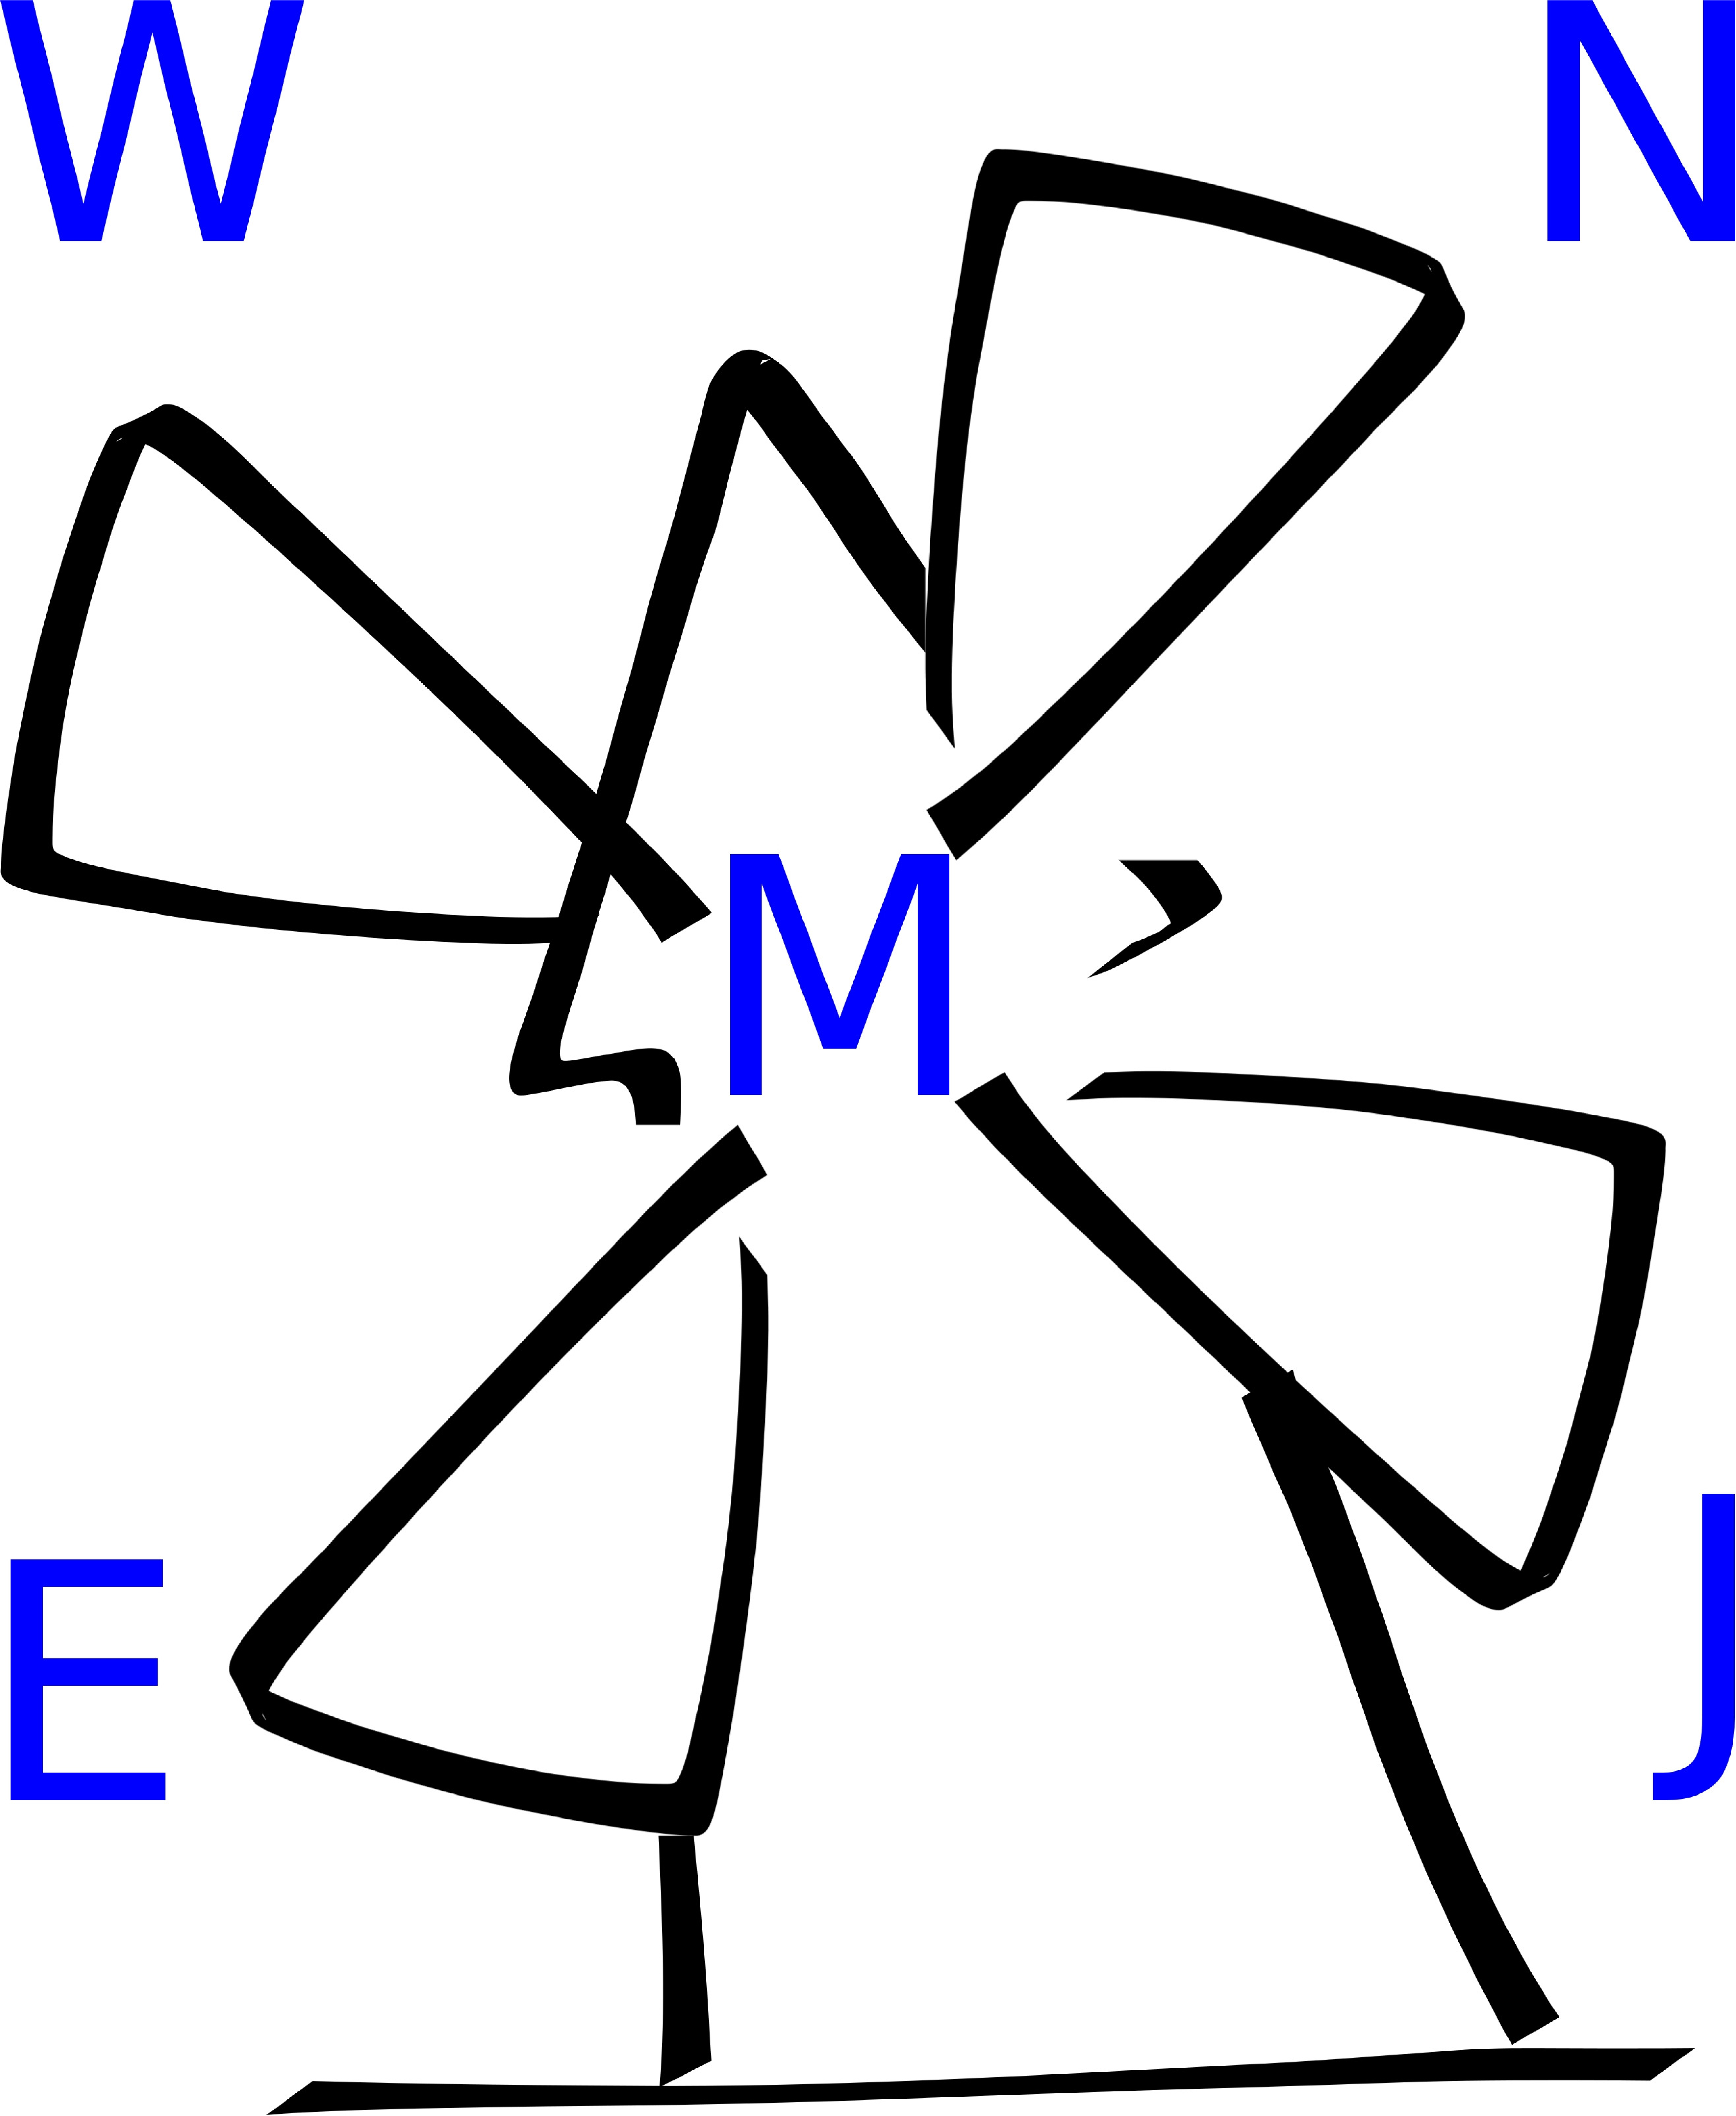
\includegraphics[height=25mm]{nwejm-logo}%
  };%
\end{tikzpicture}
\end{document}
%    \end{macrocode}
%
%    \begin{macrocode}
%</logos-collection>
%    \end{macrocode}
%
%    \begin{macrocode}
%<*bibstyle>
%    \end{macrocode}
%
%    \begin{macrocode}
\ProvidesFile{nwejm.bbx}
[2016/04/01 v 0.1 nwejm bibliographic style (DB)]

\RequireBibliographyStyle{authoryear-comp}
%    \end{macrocode}
%
% We create a name format that prints the initial(s) of the first name(s) before
% last name of a cited author.
%    \begin{macrocode}
\DeclareNameFormat{giveninits-last}{%
  \nameparts{#1}
  \usebibmacro{name:given-family}
  {\namepartfamily}
  {\namepartgiveni}
  {\namepartprefix}
  {\namepartsuffix}%
  \usebibmacro{name:andothers}%
}
%    \end{macrocode}
%
% The following is borrowed from Joseph Wright
% (\url{http://tex.stackexchange.com/a/5795/18401}) in order to prevent
% identical URL and DOI fields to be both displayed.
%    \begin{macrocode}
\renewbibmacro*{doi+eprint+url}{%
  \iftoggle{bbx:doi}%
  {%
    \iffieldundef{doi}%
    {}%
    {%
      \begingroup%
      \edef\URLorDOI{%
        \detokenize{http://dx.doi.org/}%
        \thefield{doi}%
      }%
      \iffieldequals{url}{\URLorDOI}%
      {\endgroup}%
      {%
        \endgroup%
        \printfield{doi}%
      }%
    }%
  }%
  {}%
  \newunit\newblock%
  \iftoggle{bbx:eprint}%
  {\usebibmacro{eprint}}%
  {}%
  \newunit\newblock%
  \iftoggle{bbx:url}%
  {\usebibmacro{url+urldate}}%
  {}%
}
%    \end{macrocode}
%
% We perform some other modifications to ×authoryear× bib style.
%    \begin{macrocode}
\renewbibmacro{in:}{%
  \ifentrytype{article}{}{\printtext{\bibstring{in}\intitlepunct}}%
}
\renewbibmacro*{journal}{%
  \iffieldundef{shortjournal}%
  {%
    \iffieldundef{journaltitle}%
    {}%
    {%
      \printtext[journaltitle]%
      {%
        \printfield[titlecase]{journaltitle}%
        \setunit{\subtitlepunct}%
        \printfield[titlecase]{journalsubtitle}%
      }%
    }%
  }%
  {\printtext[journaltitle]{\printfield[titlecase]{shortjournal}}}%
}
\renewbibmacro*{volume+number+eid}{%
  \printfield{volume}%
  \setunit*{\addnbthinspace}%
  \printfield{number}%
  \setunit{\addcomma\space}%
  \printfield{eid}%
}
\DeclareFieldFormat[article]{volume}{\mkbibbold{#1}}
\DeclareFieldFormat[book]{volume}{\mkbibbold{#1}}
\DeclareFieldFormat[article]{number}{\mkbibparens{#1}}
%    \end{macrocode}
%
% We redefine the label date in order the pubstate is used in case no date is
% provided (e.g. for references to appear).
%    \begin{macrocode}
\DeclareLabeldate{%
  \field{year}%
  \field{date}%
  \field{eventdate}%
  \field{origdate}%
  \field{urldate}%
  \field{pubstate}%
  \literal{nodate}%
}
%    \end{macrocode}
%
% We ensure the space between initial(s) and last name is unbreakable.
%    \begin{macrocode}
\renewcommand*\bibnamedelimc{\addnbspace}
\renewcommand*\bibnamedelimd{\addnbspace}
%    \end{macrocode}
%
% A temporary trick in order to avoid inappropriate capitalization of the
% initial after periods abbreviating journals (see
% \url{https://github.com/plk/biblatex/issues/851}).
%    \begin{macrocode}
\DeclareFieldFormat{journaltitle}{\mkbibemph{#1\isdot}}
%    \end{macrocode}
%
%    \begin{macrocode}
%</bibstyle>
%    \end{macrocode}
%
%    \begin{macrocode}
%<*citestyle>
%    \end{macrocode}
%
%    \begin{macrocode}
\ProvidesFile{nwejm.cbx}
[2016/04/01 v 0.1 nwejm citation style (DB)]

\RequireCitationStyle{authoryear-comp}

\ExecuteBibliographyOptions{giveninits,ibidtracker=constrict,pagetracker=page}

%    \end{macrocode}
%
% We redefine the ×\blx@mkbibfootnote× macro in order the footnote mark of
% bibliographic citations are in bold, just by inserting a patch of
% ×\@makefnmark×.
%    \begin{macrocode}
\renewrobustcmd{\blx@mkbibfootnote}[2]{%
  \iftoggle{blx@footnote}%
  {\blx@warning{Nested notes}%
    \addspace\mkbibparens{#2}}%
  {\unspace%
    \ifnum\blx@notetype=\tw@%
    \expandafter\@firstoftwo%
    \else%
    \expandafter\@secondoftwo%
    \fi%
    {\csuse{blx@theendnote#1}{\protecting{\blxmkbibnote{end}{#2}}}}%
    {%
      \patchcmd\@makefnmark%
      {\normalfont}%
      {\normalfont\bfseries}%
      {}{}%
      \csuse{footnote#1}{\protecting{\blxmkbibnote{foot}{#2}}}%
    }%
  }%
}
%    \end{macrocode}
%
% We also redefine the command that is responsible of the \pkg{csquotes}'
% quotations without formal citations (e.g. ×displayquote× versus
% ×displaycquote× environments).
%    \begin{macrocode}
\renewcommand*{\mkcitation}[1]{%
  \patchcmd\@makefnmark%
  {\normalfont}%
  {\normalfont\bfseries}%
  {}{}%
  \footnote{#1}%
}
%    \end{macrocode}
%
% Because this cite style is a mix between ×authortitle× and ×authoryear× but is
% mainly based upon ×authoryear× style, we need to define the bib macro
% ×cite:title× defined in ×authortitle× but not in ×authoryear×.
%    \begin{macrocode}
\newbibmacro*{cite:title}{%
    \printfield[citetitle]{labeltitle}}
%    \end{macrocode}
%
% Because we want to replace autocite redundant consecutive citations by
% \enquote{Ibid.}, we need to borrow some code from \pkg{biblatex}'s ×*-ibid* styles.
%    \begin{macrocode}
\providecommand*{\mkibid}[1]{#1}
\newbibmacro*{cite:ibid}{%
  \printtext[bibhyperref]{\bibstring[\mkibid]{ibidem}}%
}
%    \end{macrocode}
%
% We create the ×nwejm:cite× bib macro which emulates a mix between
% ×authortitle× and ×authoryear× styles: it displays the label name (mainly
% authors' names), then the year and finally the title.
%    \begin{macrocode}
\newbibmacro*{nwejm:cite}{%
  \iffieldundef{shorthand}{%
    {\ifthenelse{\ifciteibid\AND\NOT\iffirstonpage}%
      {\usebibmacro{cite:ibid}}%
      {%
        \ifthenelse{%
          \ifnameundef{labelname}%
        }{%
          \usebibmacro{cite:label}%
          \setunit{\addcomma\space}%
        }{%
          \ifthenelse{%
            \iffieldundef{labelyear}%
          }{%
            \printtext[bibhyperref]{\printnames{labelname}}%
          }{%
            \printtext[bibhyperref]{\printnames{labelname}%
            \setunit{\addcomma\space}%
            \usebibmacro{cite:labeldate+extradate}}%
            \ifthenelse{%
              \iffieldundef{labeltitle}%
            }{%
            }{%
              \setunit{\addcomma\space}%
              \usebibmacro{cite:title}%
            }%
          }%
        }%
      }%
    }%
  }{%
    \usebibmacro{cite:shorthand}%
  }%
}
%    \end{macrocode}
%
% We now declare the new cite command ×\nwejmfootcite× (and it multicite
% counterpart) which is identical to ×\footcite× except it uses the ×nwejm:cite×
% bib macro instead of the usual ×cite× one.
%    \begin{macrocode}
\DeclareCiteCommand{\nwejmfootcite}[\mkbibfootnote]
{\usebibmacro{prenote}}%
{\usebibmacro{citeindex}%
  \usebibmacro{nwejm:cite}}
{%
%    \end{macrocode}
%
% Unique (auto)citations with multiple keys are displayed in footnotes but each
% of the corresponding references is on its own line.
%    \begin{macrocode}
  \ifcurrentbaselanguage{french}{%
    \parindent=\parindentFFN%
    \addtolength{\parindent}{\widthof{\dotFFN\kernFFN}}%
  }{%
    \parindent=\footnotemargin%
  }%
  \multicitedelim\newline\indent%
}
{\usebibmacro{postnote}}%
\DeclareMultiCiteCommand{\nwejmfootcites}[\mkbibfootnote]{\nwejmfootcite}
{%
  \ifcurrentbaselanguage{french}{%
    \parindent=\parindentFFN%
    \addtolength{\parindent}{\widthof{\dotFFN\kernFFN}}%
  }{%
    \parindent=\footnotemargin%
  }%
  \multicitedelim\newline\indent%
}
%    \end{macrocode}
%
% We now declare the definitions for the ×\autocite× and ×\autocites× commands
% and we apply these definitions.
%    \begin{macrocode}
\DeclareAutoCiteCommand{nwejmfootcite}{\nwejmfootcite}{\nwejmfootcites}

\DeclareCiteCommand{\textcite}[\cbx@textcite@init\cbx@textcite]
  {\gdef\cbx@savedkeys{}%
   \citetrackerfalse%
   \pagetrackerfalse%
   \DeferNextCitekeyHook%
   \usebibmacro{cite:init}}
  {\ifthenelse{\iffirstcitekey\AND\value{multicitetotal}>0}
     {\protected@xappto\cbx@savedcites{()(\thefield{multipostnote})}%
      \global\clearfield{multipostnote}}
     {}%
   \xappto\cbx@savedkeys{\thefield{entrykey},}%
   \iffieldequals{namehash}{\cbx@lasthash}
     {}
     {\stepcounter{textcitetotal}%
      \savefield{namehash}{\cbx@lasthash}}}
  {}
  {\protected@xappto\cbx@savedcites{%
     [\thefield{prenote}][\thefield{postnote}]{\cbx@savedkeys}}}

      % \DeclareCiteCommand{\textcite}
 %  {\boolfalse{cbx:parens}}
 %  {\usebibmacro{citeindex}%
 %   \iffirstcitekey
 %     {\setcounter{textcitetotal}{1}}
 %     {\stepcounter{textcitetotal}%
 %      \textcitedelim}%
 %    \iffootnote{\usebibmacro{nwejm:cite}}{\printtext[bibhyperref]{\usebibmacro{textcite}}}}
 %  {\ifbool{cbx:parens}
 %     {\bibcloseparen\global\boolfalse{cbx:parens}}
 %     {}}
 %  {\usebibmacro{textcite:postnote}}
%    \end{macrocode}
%
%    \begin{macrocode}
\ExecuteBibliographyOptions{autocite=nwejmfootcite}
%    \end{macrocode}
%
%    \begin{macrocode}
%</citestyle>
%    \end{macrocode}
%
%    \begin{macrocode}
%<*latexmkrc>
%    \end{macrocode}
%
%    \begin{macrocode}
$pdf_mode = 1;

$bibtex_use = 1;
$bibtex = 'biber -U %O %B';

$makeindex = 'texindy -L english';

push @generated_exts, "aux", "idx", "ind", "lo*", "out", "toc", "acn", "acr",
"alg", "bbl", "bcf", "fls", "gl*", "ist", "run.xml", "sbl*", "sl*", "sym*",
"xdy", "unq", "mw", "*~" "sta" ;

$clean_ext = "synctex.gz* run.xml tex.bak bbl bcf fdb_latexmk run tdo listing sta"
%    \end{macrocode}
%
%    \begin{macrocode}
%</latexmkrc>
%    \end{macrocode}
%
% \chapter{Completion files for TeXstudio and friends}
% Now, the \file{nwejmart.cwl} and \file{nwejm.cwl} files for commands
% completion and syntax checking:
%
%    \begin{macrocode}
%<*class-cwl>
%    \end{macrocode}
%
%    \begin{macrocode}
# mode: nwejm.cls
# denisbitouze, 23.12.2015
#
#include:class-book
#include:latex-document
#include:latex-mathsymbols
#include:tex
#include:xparse
#include:l3keys2e
#include:nag
#include:graphicx
#include:adjustbox
#include:tcolorbox
#include:csquotes
#include:array
#include:booktabs
#include:mathtools
#include:ntheorem
#include:esvect
#include:kpfonts
#include:translations
#include:babel
#include:varioref
#include:subcaption
#include:tocvsec2
#include:etoc
#include:microtype
#include:datetime2
#include:enumitem
#include:biblatex
#include:hyperref
#include:hypcap
#include:bookmark
#include:glossaries
#include:cleveref
#
# Document class
#keyvals:\documentclass/nwejmart
french
english
ngerman
dutch
#endkeyvals
#
# Cover and title pages
#
# Title, etc.
\title{title}#n
\title[short title]{title}#n
\subtitle{%<subtitle%>}#n*
\subtitle[%<short subtitle%>]{%<subtitle%>}#n*
#
# Author
\author{%<Last name%>, %<First name%>}#n
\author[affiliation={%<affiliation%>}]{%<Last name%>, %<First name%>}#n
\author[affiliation=[%<affiliation's tag%>]{%<affiliation%>}]{%<Last name%>, %<First name%>}#n
\author[affiliationtagged={%<affiliation's tag%>}]{%<Last name%>, %<First name%>}#n
#
# Dates
\dates{received=%<yyyy%>-%<mm%>-%<dd%>,accepted=%<yyyy%>-%<mm%>-%<dd%>,online=%<yyyy%>-%<mm%>-%<dd%>}#n
#
# Math commands
\N#m
\Z#m
\D#m
\Q#m
\R#m
\C#m
\K#m
\arccosh#m
\arcsin#m
\arcsinh#m
\arctan#m
\arctanh#m
\Argch#m
\Argsh#m
\Argth#m
\ch#m
\cotan#m
\curl#m
\dif#m
\Div#m
\grad#m
\E#m
\I#m
\rot#m
\sh#m
\supp#m
\th#m
\norm#m
\lnorm#m
\llnorm#m
\lpnorm#m
\supnorm#m
\abs#m
\prt#m
\brk#m
\brc#m
\leqgeq#m
\lrangle#m
\set{%<set self-contained definition%>}#m
\set{%<set definition%>}[%<such that...%>]#m
\begin{axiom}
\begin{assertions}
\begin{conjecture}
\begin{corollary}
\begin{definition}
\begin{example}
\begin{hypotheses}
\begin{proposition}
\begin{lemma}
\begin{notation}
\begin{proof}
\begin{remark}
\begin{theorem}
#
\begin{axiom*}
\begin{assertions*}
\begin{conjecture*}
\begin{corollary*}
\begin{definition*}
\begin{example*}
\begin{hypotheses*}
\begin{proposition*}
\begin{lemma*}
\begin{notation*}
\begin{proof*}
\begin{remark*}
\begin{theorem*}
#
\end{axiom}
\end{assertions}
\end{conjecture}
\end{corollary}
\end{definition}
\end{example}
\end{hypotheses}
\end{proposition}
\end{lemma}
\end{notation}
\end{proof}
\end{remark}
\end{theorem}
#
\end{axiom*}
\end{assertions*}
\end{conjecture*}
\end{corollary*}
\end{definition*}
\end{example*}
\end{hypotheses*}
\end{proposition*}
\end{lemma*}
\end{notation*}
\end{proof*}
\end{remark*}
\end{theorem*}
#
\begin{description*}
\begin{enumerate*}
\begin{itemize*}
#
\end{description*}
\end{enumerate*}
\end{itemize*}
# Miscellaneous commands
\keywords{%<list of keywords%>}#n
\msc{%<list of MSCs%>}#n
\nwejm#n
\nwejm*#n*
\century{%<(positive or negative) integer%>}#n
\century*{%<(positive or negative) integer%>}#n*
\aside{%<interpolated clause%>}#n
\aside*{%<interpolated clause%>}#n
\acknowledgements{%<acknowledgments%>}#n
\ie#n
\ie*#n*
\Ie#n
\Ie*#n*
\NewPairedDelimiter#n
\articlesetup#n
\BinaryOperators#n
#
\editorinchief{%<Last name%>, %<First name%>}{%<affiliation%>}{%<country%>}{%<email%>}#n
\editor{%<Last name%>, %<First name%>}{%<affiliation%>}{%<country%>}{%<email%>}#n
\fieldseditor{%<Last name%>, %<First name%>}{%<affiliation%>}{%<country%>}{%<email%>}#n
\managingeditor{%<Last name%>, %<First name%>}{%<affiliation%>}{%<country%>}{%<email%>}#n
\classdesigner{%<Last name%>, %<First name%>}{%<affiliation%>}{%<country%>}{%<email%>}#n
\computerengineer{%<Last name%>, %<First name%>}{%<affiliation%>}{%<country%>}{%<email%>}#n
\classmaintainer{%<Last name%>, %<First name%>}{%<affiliation%>}{%<country%>}{%<email%>}#n
\fontdesigner{%<Last name%>, %<First name%>}{%<affiliation%>}{%<country%>}{%<email%>}#n
\graphicdesign{%<Last name%>, %<First name%>}{%<affiliation%>}{%<country%>}{%<email%>}#n
\computerassistance{%<Last name%>, %<First name%>}{%<affiliation%>}{%<country%>}{%<email%>}#n
\secretary{%<Last name%>, %<First name%>}{%<affiliation%>}{%<country%>}{%<email%>}#n
\issuesetup{number=%<positive integer%>}#n
\journalsetup {publisher=%<publisher%>,address={%<address%>},phone=%<phone%>,email=%<email%>,url=%<url%>,issn=%<issn%>,isbn=%<isbn%>}#n
\inputarticle{file}#i
\inputarticle[path]{file}#i
\fontdesignertext{text}#n
\graphicdesigntext{text}#n
%    \end{macrocode}
%
%    \begin{macrocode}
%</class-cwl>
%    \end{macrocode}
%
%    \begin{macrocode}
%<*classart-cwl>
%    \end{macrocode}
%
%    \begin{macrocode}
# mode: nwejm.cls
# denisbitouze, 23.12.2015
#
#include:nwejm
%    \end{macrocode}
%
%    \begin{macrocode}
%<classart-cwl>
%    \end{macrocode}
%
%    \begin{macrocode}
\endinput
%    \end{macrocode}
%
% \Finale

%%% Local Variables:
%%% mode: doctex
%%% ispell-local-dictionary: "english"
%%% TeX-command-default: "TeX"
%%% TeX-master: t
%%% End:
